%% LaTeX Template for ISIT 2024
%%
%% by Stefan M. Moser, October 2017
%% (with some modifications by Tobias Koch, November 2023)
%% 
%% derived from bare_conf.tex, V1.4a, 2014/09/17, by Michael Shell
%% for use with IEEEtran.cls version 1.8b or later
%%
%% Support sites for IEEEtran.cls:
%%
%% http://www.michaelshell.org/tex/ieeetran/
%% http://moser-isi.ethz.ch/manuals.html#eqlatex
%% http://www.ctan.org/tex-archive/macros/latex/contrib/IEEEtran/
%%

\documentclass[conference,letterpaper]{IEEEtran}

\usepackage{epsfig}
\usepackage{times}
\usepackage{float}
\usepackage{stfloats}
\usepackage{afterpage}

\usepackage{amstext,cite}
\usepackage{amssymb,bm}
\usepackage{latexsym}
\usepackage{color}
\usepackage{graphicx}


\usepackage{amsthm}
\usepackage{graphicx}
\usepackage[center]{caption}
\usepackage{pstricks}
%\usepackage{subfig}
\usepackage{caption}
\usepackage{subcaption}
\usepackage{booktabs}
\usepackage{multicol}
\usepackage{lipsum}% dummy text
\usepackage[T1]{fontenc}
%\UseRawInputEncoding
%\usepackage{mathabx}
\usepackage{hyperref}
 \usepackage{aecompl}
 \usepackage{mathrsfs}
\usepackage{arydshln}  % 导入用于虚线分隔的包




%
\setlength\unitlength{1mm}

\newcommand{\insertfig}[3]{
\begin{figure}[htbp]\begin{center}\begin{picture}(120,90)
\put(0,-5){\includegraphics[width=12cm,height=9cm,clip=]{#1.eps}}\end{picture}\end{center}
\caption{#2}\label{#3}\end{figure}}

\newcommand{\insertxfig}[4]{
\begin{figure}[htbp]
\begin{center}
\leavevmode \centerline{\resizebox{#4\textwidth}{!}{\input
#1.pstex_t}}
%\vspace*{-0.2in}
\caption{#2} \label{#3}
\end{center}
\end{figure}}

\long\def\comment#1{}

% bb font symbols

\newfont{\bbb}{msbm10 scaled 700}
\newcommand{\CCC}{\mbox{\bbb C}}

\newfont{\bb}{msbm10 scaled 1100}
\newcommand{\CC}{\mbox{\bb C}}
\newcommand{\PP}{\mbox{\bb P}}
\newcommand{\RR}{\mbox{\bb R}}
\newcommand{\QQ}{\mbox{\bb Q}}
\newcommand{\ZZ}{\mbox{\bb Z}}
\newcommand{\FF}{\mbox{\bb F}}
\newcommand{\GG}{\mbox{\bb G}}
\newcommand{\EE}{\mbox{\bb E}}
\newcommand{\NN}{\mbox{\bb N}}
\newcommand{\KK}{\mbox{\bb K}}

% Vectors

\newcommand{\av}{{\bf a}}
\newcommand{\bv}{{\bf b}}
\newcommand{\cv}{{\bf c}}
\newcommand{\dv}{{\bf d}}
\newcommand{\ev}{{\bf e}}
\newcommand{\fv}{{\bf f}}
\newcommand{\gv}{{\bf g}}
\newcommand{\hv}{{\bf h}}
\newcommand{\iv}{{\bf i}}
\newcommand{\jv}{{\bf j}}
\newcommand{\kv}{{\bf k}}
\newcommand{\lv}{{\bf l}}
\newcommand{\mv}{{\bf m}}
\newcommand{\nv}{{\bf n}}
\newcommand{\ov}{{\bf o}}
\newcommand{\pv}{{\bf p}}
\newcommand{\qv}{{\bf q}}
\newcommand{\rv}{{\bf r}}
\newcommand{\sv}{{\bf s}}
\newcommand{\tv}{{\bf t}}
\newcommand{\uv}{{\bf u}}
\newcommand{\wv}{{\bf w}}
\newcommand{\vv}{{\bf v}}
\newcommand{\xv}{{\bf x}}
\newcommand{\yv}{{\bf y}}
\newcommand{\zv}{{\bf z}}
\newcommand{\zerov}{{\bf 0}}
\newcommand{\onev}{{\bf 1}}

% Matrices

\newcommand{\Am}{{\bf A}}
\newcommand{\Bm}{{\bf B}}
\newcommand{\Cm}{{\bf C}}
\newcommand{\Dm}{{\bf D}}
\newcommand{\Em}{{\bf E}}
\newcommand{\Fm}{{\bf F}}
\newcommand{\Gm}{{\bf G}}
\newcommand{\Hm}{{\bf H}}
\newcommand{\Id}{{\bf I}}
\newcommand{\Jm}{{\bf J}}
\newcommand{\Km}{{\bf K}}
\newcommand{\Lm}{{\bf L}}
\newcommand{\Mm}{{\bf M}}
\newcommand{\Nm}{{\bf N}}
\newcommand{\Om}{{\bf O}}
\newcommand{\Pm}{{\bf P}}
\newcommand{\Qm}{{\bf Q}}
\newcommand{\Rm}{{\bf R}}
\newcommand{\Sm}{{\bf S}}
\newcommand{\Tm}{{\bf T}}
\newcommand{\Um}{{\bf U}}
\newcommand{\Wm}{{\bf W}}
\newcommand{\Vm}{{\bf V}}
\newcommand{\Xm}{{\bf X}}
\newcommand{\Ym}{{\bf Y}}
\newcommand{\Zm}{{\bf Z}}

% Calligraphic

\newcommand{\Ac}{{\cal A}}
\newcommand{\Bc}{{\cal B}}
\newcommand{\Cc}{{\cal C}}
\newcommand{\Dc}{{\cal D}}
\newcommand{\Ec}{{\cal E}}
\newcommand{\Fc}{{\cal F}}
\newcommand{\Gc}{{\cal G}}
\newcommand{\Hc}{{\cal H}}
\newcommand{\Ic}{{\cal I}}
\newcommand{\Jc}{{\cal J}}
\newcommand{\Kc}{{\cal K}}
\newcommand{\Lc}{{\cal L}}
\newcommand{\Mc}{{\cal M}}
\newcommand{\Nc}{{\cal N}}
\newcommand{\Oc}{{\cal O}}
\newcommand{\Pc}{{\cal P}}
\newcommand{\Qc}{{\cal Q}}
\newcommand{\Rc}{{\cal R}}
\newcommand{\Sc}{{\cal S}}
\newcommand{\Tc}{{\cal T}}
\newcommand{\Uc}{{\cal U}}
\newcommand{\Wc}{{\cal W}}
\newcommand{\Vc}{{\cal V}}
\newcommand{\Xc}{{\cal X}}
\newcommand{\Yc}{{\cal Y}}
\newcommand{\Zc}{{\cal Z}}

% Bold greek letters

\newcommand{\alphav}{\hbox{\boldmath$\alpha$}}
\newcommand{\betav}{\hbox{\boldmath$\beta$}}
\newcommand{\gammav}{\hbox{\boldmath$\gamma$}}
\newcommand{\deltav}{\hbox{\boldmath$\delta$}}
\newcommand{\etav}{\hbox{\boldmath$\eta$}}
\newcommand{\lambdav}{\hbox{\boldmath$\lambda$}}
\newcommand{\epsilonv}{\hbox{\boldmath$\epsilon$}}
\newcommand{\nuv}{\hbox{\boldmath$\nu$}}
\newcommand{\muv}{\hbox{\boldmath$\mu$}}
\newcommand{\zetav}{\hbox{\boldmath$\zeta$}}
\newcommand{\phiv}{\hbox{\boldmath$\phi$}}
\newcommand{\psiv}{\hbox{\boldmath$\psi$}}
\newcommand{\thetav}{\hbox{\boldmath$\theta$}}
\newcommand{\tauv}{\hbox{\boldmath$\tau$}}
\newcommand{\omegav}{\hbox{\boldmath$\omega$}}
\newcommand{\xiv}{\hbox{\boldmath$\xi$}}
\newcommand{\sigmav}{\hbox{\boldmath$\sigma$}}
\newcommand{\piv}{\hbox{\boldmath$\pi$}}
\newcommand{\rhov}{\hbox{\boldmath$\rho$}}

\newcommand{\Gammam}{\hbox{\boldmath$\Gamma$}}
\newcommand{\Lambdam}{\hbox{\boldmath$\Lambda$}}
\newcommand{\Deltam}{\hbox{\boldmath$\Delta$}}
\newcommand{\Sigmam}{\hbox{\boldmath$\Sigma$}}
\newcommand{\Phim}{\hbox{\boldmath$\Phi$}}
\newcommand{\Pim}{\hbox{\boldmath$\Pi$}}
\newcommand{\Psim}{\hbox{\boldmath$\Psi$}}
\newcommand{\Thetam}{\hbox{\boldmath$\Theta$}}
\newcommand{\Omegam}{\hbox{\boldmath$\Omega$}}
\newcommand{\Xim}{\hbox{\boldmath$\Xi$}}


% Sans Serif small case

\newcommand{\asf}{{\sf a}}
\newcommand{\bsf}{{\sf b}}
\newcommand{\csf}{{\sf c}}
\newcommand{\dsf}{{\sf d}}
\newcommand{\esf}{{\sf e}}
\newcommand{\fsf}{{\sf f}}
\newcommand{\gsf}{{\sf g}}
\newcommand{\hsf}{{\sf h}}
\newcommand{\isf}{{\sf i}}
\newcommand{\jsf}{{\sf j}}
\newcommand{\ksf}{{\sf k}}
\newcommand{\lsf}{{\sf l}}
\newcommand{\msf}{{\sf m}}
\newcommand{\nsf}{{\sf n}}
\newcommand{\osf}{{\sf o}}
\newcommand{\psf}{{\sf p}}
\newcommand{\qsf}{{\sf q}}
\newcommand{\rsf}{{\sf r}}
\newcommand{\ssf}{{\sf s}}
\newcommand{\tsf}{{\sf t}}
\newcommand{\usf}{{\sf u}}
\newcommand{\wsf}{{\sf w}}
\newcommand{\vsf}{{\sf v}}
\newcommand{\xsf}{{\sf x}}
\newcommand{\ysf}{{\sf y}}
\newcommand{\zsf}{{\sf z}}

% Sans Serif large case

\newcommand{\Asf}{{\sf A}}
\newcommand{\Bsf}{{\sf B}}
\newcommand{\Csf}{{\sf C}}
\newcommand{\Dsf}{{\sf D}}
\newcommand{\Esf}{{\sf E}}
\newcommand{\Fsf}{{\sf F}}
\newcommand{\Gsf}{{\sf G}}
\newcommand{\Hsf}{{\sf H}}
\newcommand{\Isf}{{\sf I}}
\newcommand{\Jsf}{{\sf J}}
\newcommand{\Ksf}{{\sf K}}
\newcommand{\Lsf}{{\sf L}}
\newcommand{\Msf}{{\sf M}}
\newcommand{\Nsf}{{\sf N}}
\newcommand{\Osf}{{\sf O}}
\newcommand{\Psf}{{\sf P}}
\newcommand{\Qsf}{{\sf Q}}
\newcommand{\Rsf}{{\sf R}}
\newcommand{\Ssf}{{\sf S}}
\newcommand{\Tsf}{{\sf T}}
\newcommand{\Usf}{{\sf U}}
\newcommand{\Wsf}{{\sf W}}
\newcommand{\Vsf}{{\sf V}}
\newcommand{\Xsf}{{\sf X}}
\newcommand{\Ysf}{{\sf Y}}
\newcommand{\Zsf}{{\sf Z}}


% mixed symbols

\newcommand{\sinc}{{\hbox{sinc}}}
\newcommand{\diag}{{\hbox{diag}}}
\renewcommand{\det}{{\hbox{det}}}
\newcommand{\trace}{{\hbox{tr}}}
\newcommand{\sign}{{\hbox{sign}}}
\renewcommand{\arg}{{\hbox{arg}}}
\newcommand{\var}{{\hbox{var}}}
\newcommand{\cov}{{\hbox{cov}}}
\newcommand{\SINR}{{\sf SINR}}
\newcommand{\SNR}{{\sf SNR}}
\newcommand{\Ei}{{\rm E}_{\rm i}}
\renewcommand{\Re}{{\rm Re}}
\renewcommand{\Im}{{\rm Im}}
\newcommand{\eqdef}{\stackrel{\Delta}{=}}
\newcommand{\defines}{{\,\,\stackrel{\scriptscriptstyle \bigtriangleup}{=}\,\,}}
\newcommand{\<}{\left\langle}
\renewcommand{\>}{\right\rangle}
\newcommand{\herm}{{\sf H}}
\newcommand{\trasp}{{\sf T}}
\newcommand{\transp}{{\sf T}}
\renewcommand{\vec}{{\rm vec}}
%\newcommand{\Psf}{{\sf P}}
%\newcommand{\mod}{{\rm mod}}

% equations
\newcommand{\be}{\begin{equation}}
\newcommand{\ee}{\end{equation}}
\newcommand{\bea}{\begin{eqnarray}}
\newcommand{\eea}{\end{eqnarray}}
\newtheorem{thm}{Theorem}%[section]
\newtheorem{cor}{Corollary}
\newtheorem{lem}{Lemma}
\newtheorem{prop}{Proposition}
\newtheorem{rem}{Remark}
\newtheorem{example}{Example}
\newtheorem{defn}{\protect\definitionname}

% Colors

\newcommand{\RED}{\color[rgb]{1.00,0.10,0.10}}
\newcommand{\BLUE}{\color[rgb]{0,0,0.90}}
\newcommand{\GREEN}{\color[rgb]{0,0.80,0.20}}

%%%%%%%%%%%%%%%%%%%%%%%%%%%%%%%%%%%%%%%%%%%%%%%%%
\def\MSE    {\mbox{\scriptsize\sf MSE}}
\def\Fsf{ {\sf F}}
\def\E{{\mathbb E}}
\def \Acomp {{A}}
\def\fsf{ {\sf f}}
\def\tr{{\rm tr}}
\def \Idm{{\bf I }}
\def\Var{{\rm Var}}
\def\pdf{{\rm p.d.f. }}

%% depending on your installation, you may wish to adjust the top margin:
\addtolength{\topmargin}{9mm}

%%%%%%
%% Packages:
%% Some useful packages (and compatibility issues with the IEEE format)
%% are pointed out at the very end of this template source file (they are 
%% taken verbatim out of bare_conf.tex by Michael Shell).
%
% *** Do not adjust lengths that control margins, column widths, etc. ***
% *** Do not use packages that alter fonts (such as pslatex).         ***
%
\usepackage[utf8]{inputenc} 
\usepackage[T1]{fontenc}
\usepackage{url}
\usepackage{ifthen}
\usepackage{cite}
\usepackage[cmex10]{amsmath} % Use the [cmex10] option to ensure complicance
                             % with IEEE Xplore (see bare_conf.tex)

\newcommand{\dt}[1]{{\blue #1}}
\newcommand{\NEW}[1]{{\red #1}}


\usepackage{amsmath}
\usepackage{tikz}
\usetikzlibrary{calc}

\usepackage[nodisplayskipstretch]{setspace} %\setstretch{1.5}

% Define tikzmark and DrawboxF for multi-line box and labels
\newcommand{\tikzmark}[1]{\tikz[overlay,remember picture] \node (#1) {};}
% 定义第一个框命令 \DrawboxF
\newcommand{\DrawboxF}[4][]{%
    \tikz[overlay,remember picture]{%
        \coordinate (TopLeft)     at ($(#2)+(-0.2em,1.5em)$); % 调整顶部和底部坐标
        \coordinate (BottomRight) at ($(#3)+(0.2em,-2.5em)$); % 
        %
        \path (TopLeft); \pgfgetlastxy{\XCoord}{\IgnoreCoord};
        \path (BottomRight); \pgfgetlastxy{\IgnoreCoord}{\YCoord};
        \coordinate (LabelPoint) at ($(\XCoord,\YCoord)!0.5!(BottomRight)$);
        %
        \draw [#1, dashed] (TopLeft) rectangle (BottomRight); % 绘制虚线框
       \node [#1, fill=none, fill opacity=1] at ([xshift=-2em, yshift=-6pt]BottomRight.south) {#4};
    }
}

% 定义第二个框命令 \DrawboxV
\newcommand{\DrawboxV}[4][]{%
    \tikz[overlay,remember picture]{%
        \coordinate (TopLeft)     at ($(#2)+(-0.2em,1.5em)$);
        \coordinate (BottomRight) at ($(#3)+(0.2em,-3.5em)$); % 这里增加了下延伸距离
        %
        \path (TopLeft); \pgfgetlastxy{\XCoord}{\IgnoreCoord};
        \path (BottomRight); \pgfgetlastxy{\IgnoreCoord}{\YCoord};
        \coordinate (LabelPoint) at ($(\XCoord,\YCoord)!0.5!(BottomRight)$);
        %
        \draw [#1, dashed] (TopLeft) rectangle (BottomRight);
       \node [#1, fill=none, fill opacity=1] at ([xshift=-2em, yshift=-10pt]BottomRight.south) {#4};
    }
}

 \setlength {\marginparwidth }{2cm} 
 \newcommand{\DrawBox}[4][]{%
    \tikz[overlay,remember picture]{%
        \coordinate (TopLeft)     at ($(#2)+(-0.2em,0.9em)$);
        \coordinate (BottomRight) at ($(#3)+(0.2em,-0.3em)$);
        %
        \path (TopLeft); \pgfgetlastxy{\XCoord}{\IgnoreCoord};
        \path (BottomRight); \pgfgetlastxy{\IgnoreCoord}{\YCoord};
        \coordinate (LabelPoint) at ($(\XCoord,\YCoord)!0.5!(BottomRight)$);
        %
        \draw [red,#1] (TopLeft) rectangle (BottomRight);
        \node [below, #1, fill=none, fill opacity=1] at (LabelPoint) {#4};
    }
}


%% Please note that the amsthm package must not be loaded with
%% IEEEtran.cls because IEEEtran provides its own versions of
%% theorems. Also note that IEEEXplore does not accepts submissions
%% with hyperlinks, i.e., hyperref cannot be used.

\interdisplaylinepenalty=2500 % As explained in bare_conf.tex


%%%%%%
% correct bad hyphenation here
\hyphenation{op-tical net-works semi-conduc-tor}

% ------------------------------------------------------------
\begin{document}
\title{The Key Size of Secure Aggregation In Distributed Linearly  Separable Computation} 

% %%% Single author, or several authors with same affiliation:
% \author{%
%  \IEEEauthorblockN{Andrew R.~Barron}
%  \IEEEauthorblockA{Department of Statistics and Data Science\\
%                    Yale University\\
%                    New Haven, CT, USA\\
%                    Email: andrew.barron@yale.edu}
% }


%%% Several authors with up to three affiliations:
\author{%
  \IEEEauthorblockN{Yang Zhou, Wenbo Huang}
  \IEEEauthorblockA{The School of Electronic Information and Communications,\\
                    Huangzhong University of Science and Technology at Wuhan,\\
                    430074 Wuhan, China\\
                    Email: \{hust\_zhou, eric\_huang\}@hust.edu.cn}
  \and
  \IEEEauthorblockN{Claude E.~Shannon and David Slepian}
  \IEEEauthorblockA{Bell Telephone Laboratories, Inc.\\ 
                    Murray Hill, NJ, USA\\
                    Email: \{csh, dsl\}@bell-labs.com}
}


%%% Many authors with many affiliations:
% \author{%
%   \IEEEauthorblockN{Andrew R.~Barron\IEEEauthorrefmark{1},
%                     Claude E.~Shannon\IEEEauthorrefmark{2},
%                     David Slepian\IEEEauthorrefmark{2},
%                     and Jacob Ziv\IEEEauthorrefmark{2}\IEEEauthorrefmark{3}}
%   \IEEEauthorblockA{\IEEEauthorrefmark{1}%
%                    Department of Statistics and Data Science, Yale University, New Haven, CT, USA,
%                     andrew.barron@yale.edu}
%   \IEEEauthorblockA{\IEEEauthorrefmark{2}%
%                     Bell Telephone Laboratories, Inc.,
%                     Murray Hill, NJ, USA,
%                     \{csh,dsl,jz\}@bell-labs.com}
%   \IEEEauthorblockA{\IEEEauthorrefmark{3}%
%                     Department of Electrical Engineering, Technion---Institute of Technology, Haifa, Israel,
%                     jz@ee.technion.ac.il}
% }


\maketitle

%%%%%%
%% Abstract: 
%% If your paper is eligible for the student paper award, please add
%% the comment "THIS PAPER IS ELIGIBLE FOR THE STUDENT PAPER
%% AWARD." as a first line in the abstract. 
%% For the final version of the accepted paper, please do not forget
%% to remove this comment!
%%

\begin{abstract}
Secure aggregation has been a key focus in distributed computation and is becoming increasingly important with the growth of distributed machine learning. In this paper, we discuss secure aggregation in a well-known distributed computation scenario called Distributed Linearly Separable Computation.  We focus on the two key factors that affect the communication cost and storage cost in the secure distributed linearly separable computation problem: key size and individual key size.
 We first propose a computing scheme that achieves the minimum individual key size under the optimal communication cost. The proposed scheme reduces the overhead associated with key storage and transmission, which are essential considerations in secure aggregation protocols. 
Then we research the minimum key size under general computation cost while achieving optimal communication cost. For this purpose, we propose a new computing scheme with a novel assignment strategy.
%, which is also applicable to the case of minimal computational cost in \cite{wan2022secure}.

\iffalse
The master asks the workers to compute some linearly separable function while ensuring security. The data center assigns an unencoded subset of the input datasets to each worker, and each worker computes some encoded packets on the assigned datasets and sends them to the master. To protect the security of the input datasets, some dataset-independent keys should be introduced in the transmission. This allows the master to obtain the required task functions from the responses of the surviving subset of servers in the presence of stragglers without obtaining any other information about the input datasets. In this paper, we focus on the general case (i.e., multiple task functions and general computational cost), aiming to find the minimum key size while achieving the optimal communication cost. In addition, we explore the minimum key size (i.e., individual key size) that needs to be stored by each worker in case the task function varies. We first present the converse bound for the individual key size under the constraints of the cyclic assignment, which is widely considered in the literature. We propose a novel distributed computation scheme for certain system parameters to reach the converse bound on the individual key size.
\fi
\end{abstract}

\begin{IEEEkeywords}
    Distributed Linearly Separable Computation, Secure Aggregation, Key Size    
\end{IEEEkeywords}
    



\section{Introduction}

Secure aggregation is a well-established topic in distributed computation, referring to the multiparty computation problem where the task is to compute a multiparty sum while no party reveals its update in the clear, not even to the aggregator~\cite{Bonawitz_Secure_Aggregation}. The concept of secret sharing was first introduced in \cite{shamir1979share}, where a secret is divided into multiple shares, and only participants meeting a threshold can reconstruct the secret. %Any group of participants below the threshold, even if they know the shares of multiple participants, cannot obtain any secret information, thereby ensuring information-theoretic security.
The complexity of verifiable secret sharing and its extension to multiparty computation were further studied in \cite{pedersen1991non, cramer2000complexity, ChaumMultiparty1988,yue2016healthcare}. Recently, secure aggregation in Federated Learning has gained significant attention \cite{fereidooni2021safe,yang2021lightsecagg,choi2020communication, jahani2022swiftagg,zhao2022information}.\cite{yang2021lightsecagg} achieves secure aggregation with only two rounds of communication, effectively reducing the communication cost.
 One of the bottlenecks of secure aggregation is key size. Based on the key size, the computation cost for key generation and the communication cost for key sharing will seriously influence the system computation capability. \cite{choi2020communication, jahani2022swiftagg} decrease the key size generated locally by each server, which in turn reduces both the computation cost and the communication cost between servers.\cite{zhao2022information} further explores the concept of individual key size, reducing the individual key size to decrease the storage cost for each server.


%{\red rewrite}


In this paper, we consider the secure aggregation in distributed linearly separable computation.
%{\blue need?} The definition of security varies across different models. 
%In the federated learning model, which is most similar to the secure distributed linearly separable computation model considered in this paper, security ensures that the server learns only the aggregated sum of the model updates from the users and no additional information about each individual’s update. {\red change location} The secure aggregation protocols proposed in \cite{fereidooni2021safe} and~\cite{Bonawitz_Secure_Aggregation} ensure this property. 
The distributed linearly separable computation was first proposed in~\cite{m=1}, which unified and extended the models of distributed gradient coding and distributed linear transformation~\cite{pmlr-v70-tandon17a,ye2018communication,Jahani2021OptimalCommunication-Computation,Short-dot}. A master wants to compute ${\bf F}[W_1; \ldots; W_{\Ksf}]$ with the help of $\Nsf$ workers, where 
$ W_k, \forall k \in [\Ksf]$ are the computation results of datasets  and \( {\bf F} \) is a demand matrix. From any $\Nsf_{\rm r}$ workers' messages, the master can complete the computation task. Each worker is assigned $\Msf = \Nsf - \Nsf_{\rm r} + \msf$ datasets, where $\msf$ is the communication reduction factor. Secure aggregation in distributed linearly separable computation ensures that the master can only retrieve the desired task function without obtaining any additional information. Formally, it can be expressed as:
\begin{align}
I\big(W_{1}, \ldots, W_{\Ksf}; X_{[\Nsf]} \mid {\bf F} [W_1; \ldots; W_{\Ksf}] \big) = 0, \label{eq:security}
\end{align}
where \( X_{[\Nsf]} \) denotes the encoded messages sent by all workers to the master. The secure aggregation of distributed linearly separable computation problem under minimum computation cost was first proposed in~\cite{wan2022secure}, and it discussed the minimum key size without increasing the communication cost.\footnote{The computation cost is defined as the number of datasets assigned to each worker, while the communication cost is defined as the number of (coded) messages that the master should receive.}   


\iffalse
{\red talk about the Distributed Linearly Separable Computation}

We mainly discuss the key size under general computation cost and individual key size stored in each worker, which has already been extensively studied in the context of federated learning models. In \cite{choi2020communication}, a sparse random graph topology design was used, while in \cite{jahani2022swiftagg}, a hierarchical aggregation architecture was implemented. Both approaches reduce the number of servers involved in the key-sharing phase, which in turn decreases the key size generated locally by each server, thereby reducing the computation cost and the communication cost between servers. The scheme proposed in \cite{zhao2022information} further explores the concept of individual key size, reducing the individual key size to decrease the storage cost for each server. 
\fi
%{\red Conclusion the importance of key size: communication cost among master-worker or workers; storage; key size -> individual key size  } 

Key size is a crucial factor affecting both the computation cost and communication cost in secure aggregation, while individual key size influences the storage cost for each participant.
%{\red Why do we discuss the key size and individual key size? } 
In the secure distributed linearly separable computation problem, all keys are shared by a third trusted server to the workers~\cite{wan2022secure}. Since the demand matrix is constantly changing in real-time applications such as those in \cite{Yu_2021_ICCV} and convolution computations \cite{cong2014minimizing}, if we follow the key distribution method proposed in \cite{wan2022secure}, the third trusted server would need to broadcast all keys to the workers. In our proposed scheme, the third trusted server sends a unique key combination to each worker at the beginning, independent of the demand matrix. It is clear that in our scheme, the third trusted server can perform key distribution without needing to know the demand.
This significantly reduces the communication cost for key sharing between the third trusted server and the workers and the storage cost for each worker.
 Moreover, our scheme achieves the optimal individual key size with minimal communication cost. We also extend the scheme in \cite{wan2022secure} to make it work for general computation cost and provide the minimum key size.


%{\red 1.Secure aggregation; 2.Distributed Linearly Separable Computation}

\iffalse
In the rapidly evolving data processing landscape, distributed computing is a pivotal solution for handling the vast computational demands of cloud and edge computing environments. As given in \cite{Speeding_Up_Distributed}, the paradigm of coded distributed computing offered robust strategies to combat the detrimental effects of stragglers, which are worker nodes that significantly delay computing and communicating gradient vectors to the master, and to curtail communication bandwidth usage.

%However, the distributed coded computing scheme proposed in~\cite{Speeding_Up_Distributed,???4-5, Short-dot}, based on linear coded data distribution, has significant limitations. 
%The model is constrained to scenarios where only linear data processing is possible due to the preprocessing step in the data center.

\cite{yu2020straggler} and \cite{Straggler_2} both focused on mitigating straggler effects in distributed matrix multiplication through coding techniques, with \cite{yu2020straggler} addressing fundamental limits and optimal coding, and \cite{Straggler_2} analyzing the optimal recovery threshold, demonstrating how coding schemes can improve system efficiency and resilience.
\cite{pmlr-v70-tandon17a} is the first to propose incorporating coding into the distributed gradient descent problem. Subsequently, \cite{ye2018communication} and \cite{Jahani2021OptimalCommunication-Computation} further investigated the trade-offs among computation cost, straggler tolerance, and communication cost within the framework of distributed gradient coding, where the computation cost is defined as the number of datasets assigned to each worker, and the communication cost refers to the number of coded messages that must be received.
The distributed linearly separable computation proposed in~\cite{m=1} unified and extended the models of distributed gradient coding \cite{pmlr-v70-tandon17a} and distributed linear transformation \cite{Short-dot}. The proposed coding scheme achieved the optimal communication cost under cyclic data assignment when the computation cost is minimized. The coding scheme in~\cite{limit} extended the scheme in \cite{m=1} to the arbitrary communication cost cases under cyclic data assignment.

The distributed linearly separable computation problem has primarily been discussed in the literature above. However, with growing concerns over information leakage, the security of distributed linearly separable computation warrants further consideration. 
The concept of information-theoretic secrecy was first introduced in \cite{Shannon}, where the minimum key size required to achieve perfect security was also established. The concept of conditionally-perfect secrecy was introduced in \cite{maurer1992conditionally}, where ciphertexts can achieve near-perfect security under certain assumptions, such as limited knowledge or computational capability of the adversary. The study explores the trade-off between key size and security by introducing randomized cipher systems.

The concept of secret sharing was first introduced in \cite{shamir1979share}, where a secret is divided into multiple shares, and only specific subsets of these shares can reconstruct the original secret. This method ensured that unauthorized subsets gain no information about the secret. The complexity of verifiable secret sharing and its extension to multiparty computation were further studied in \cite{cramer2000complexity}. These works laid the foundation for secure multiparty computation, balancing computation cost, communication cost, and security.
The definition of security varies across different models. In the federated learning model, which is most similar to the secure distributed linearly separable computation model considered in this paper, security ensures that the server learns only the aggregated sum of the model updates from the users and no additional information about each individual’s update. The secure aggregation protocols proposed in \cite{fereidooni2021safe} and~\cite{Bonawitz_Secure_Aggregation} ensure this property.


In the master-worker distributed computing model studied in this paper, security is defined as ensuring that the master retrieves only the desired task function without obtaining any additional information about the input datasets. Formally, this can be expressed as:
\begin{align}
I\big(W_{1},\ldots, W_{\Ksf}; X_{[\Nsf]} \mid {\bf F} [W_1;\ldots;W_{\Ksf}] \big) = 0, 
\end{align}
where $W_k$, corresponding to the input dataset $D_k$ for all $k \in \{1, \ldots, \Ksf\}$, is the result of applying the partial function $f_k(\cdot)$, $X_{[\Nsf]}$ denotes the encoded information sent by all workers to the master, and ${\bf F}$ is the demand matrix.
Although specific coding schemes for a single task function and minimal computation cost ($\Ksf_{\rm c}=1$ and $\Msf = \frac{\Ksf}{\Nsf}(\Nsf - \Nsf_{\rm r} + 1)$) are given in \cite{wan2022secure}, aiming to minimize the key size. However, for more general cases where the computation cost is not minimal or multiple task functions, the coding scheme for optimal key size remains open. It is worth noting that not all workers have to store all keys; they often only need to store specific linear combinations of keys, which is also to be explored in the literature.

\fi

\paragraph*{Main Contribution} 
In this paper, we focus on the secure distributed linearly separable computation problem, which prevents the master from accessing any information about the dataset besides the task function. 

%We first propose a computing scheme that achieves the minimum individual key size under the optimal communication cost.
%Then we focus on the minimum key size under general computation cost ( \( \Msf = \frac{\Ksf}{\Nsf}(\Nsf - \Nsf_{\rm r} + \msf) \)){\blue notation or delete?} while achieving optimal communication cost, and we develop the following results.

\begin{itemize}
\item We first propose a new computing scheme with a novel assignment strategy for the case $\Msf = \frac{\Ksf}{\Nsf}(\Nsf - \Nsf_{\rm r} + \msf)$. The computing scheme can cover the optimality results of the computational scheme with fractional repetition assignment; in general, it requires a smaller key size than the computing scheme with cyclic assignment while enabling optimal communication costs. The new computing scheme is also applicable to the case of minimal computational cost in \cite{wan2022secure}.   
\item We propose a computing scheme that achieves the minimum individual key size under the optimal communication cost. Based on the observation that not all workers have to store all the keys, we propose a novel secure distributed computation scheme with the constraint that $\Nsf \geq \frac{\msf+\usf-1}{\usf}+ \usf(\Nsf_{\rm r}-\msf-\usf+1)$ where $\usf:= \frac{\Ksf_{\rm c} \Nsf}{\Ksf}$. which achieves the proposed converse bound on the individual key size within this parameter.
\end{itemize}

\paragraph*{Notation Convention}
%We use the following notation convention.
Calligraphic symbols denote sets,  
bold lower-case letters denote vector, bold
upper-case letters denote matrices,
and sans-serif symbols denote system parameters.
We use $|\cdot|$ to represent the cardinality of a set or the length of a vector;
$[a:b]:=\left\{ a,a+1,\ldots,b\right\}$; %$(a:b]:=\{a+1,a+2,\ldots,b \} $, $[a:b):=\{a,a+1,\ldots,b-1 \} $, $(a,b)=\{a+1,a+2,\ldots,b-1\}$ and $[n] := [1:n]$; 
  $[n] := [1:n]$;
%$\oplus$ represents bit-wise XOR; $\mathbb{E}[\cdot]$ represents the expectation value of a random variable;  
%$a!=a\times (a-1) \times \ldots \times 1$ represents the factorial of $a$;
$\mathbb{F}_{\qsf}$ represents a  finite field with order $\qsf$;         
$\mathbf{M}^{\text{T}}$  and $\mathbf{M}^{-1}$ represent the transpose  and the inverse of matrix $\mathbf{M}$, respectively;
%$\text{rank}(\mathbf{M})$ represents the rank of matrix $\mathbf{M}$;
$\mathbf{I}_n$ represents the identity matrix with dimension $n \times n$;
${\bf 0}_{m \times n}$ represents the zero  matrix with dimension $m\times n$; 
 the matrix $[a;b]$ is written in a Matlab form, representing $[a,b]^{\text{T}}$;
$(\mathbf{M})_{m \times n}$ represents the dimension of matrix $\mathbf{M}$ is $m \times n$;
$\mathbf{M}^{(\Sc)_{\rm r}}$ represents the sub-matrix of $\mathbf{M}$ which is composed of the rows  of $\mathbf{M}$ with indices in $\Sc$ (here $\rm r$ represents `rows'); 
$\mathbf{M}^{(\Sc)_{\rm c}}$ represents the sub-matrix of $\mathbf{M}$ which is composed of the columns  of $\mathbf{M}$ with indices in $\Sc$ (here $\rm c$ represents `columns'); 
 %$\text{det}(\mathbf{M})$ represents the determinant matrix $\mathbf{M}$;
%$\mathbf{M}_{\Sc,\Vc}$ represents the sub-matrix of $\mathbf{M}$ by selecting from $\mathbf{M}$, the rows with indices in $\Sc$  and the columns with indices in $\Vc$.
 $\text{Mod} (b,a)$ represents the modulo operation on $b$ with  integer divisor $a$ and in this paper we let $\text{Mod}(b,a)\in \{1,\ldots,a \}$ (i.e., we let $ \text{Mod}(b,a)=a$ if $a$ divides $b$);
$\text{GCD}(b,a)$ represents the Greatest Common Divisor of integers $b$ and $a$;   
%the number of $k$-permutations of $n, n\geq k,$ is indicated as $P(n,k):=n\cdot(n-1)\ldots(n-k+1)$.
we let $\binom{x}{y}=0$ if $x<0$ or $y<0$ or $x<y$.
 In this paper, for each set  of integers  $\Sc$, we sort the elements in $\Sc$ in an increasing order and denote the $i^{\text{th}}$ smallest element by $\Sc(i)$, i.e., $\Sc(1)<\ldots<\Sc(|\Sc|)$.

\iffalse

\section{Related Works}
Non-secure distributed linearly separable computation has received much attention in the literature, and good results have been obtained. Its framework addresses two significant bottlenecks in distributed computing systems: communication cost and stragglers. In this computation problem, a master seeks to evaluate a linearly separable function $f$ over $\Ksf$ datasets ($D_1, \ldots, D_{\Ksf}$), defined as 
$$
f(D_1, \ldots, D_{\Ksf}) = g\big(f_1(D_1), \ldots, f_{\Ksf}(D_{\Ksf}) \big) = g(W_1, \ldots, W_{\Ksf}),
$$
where $W_k = f_k(D_k)$ represents the result of applying the partial function $f_k(\cdot)$ to the dataset $D_k$ for all $k \in \{1, \ldots, \Ksf\}$. The function $g(W_1, \ldots, W_{\Ksf})$ can be interpreted as $\Ksf_{\rm c}$ linear combinations of the messages $W_1, \ldots, W_{\Ksf}$, with coefficients that are uniformly i.i.d.
The $(\Ksf,\Nsf,\Nsf_{\rm r},\Ksf_{\rm c},\msf)$ distributed computing framework contains three phases:
  \begin{itemize}
  \item {\it Data assignment phase.} The master assigns the datasets to the workers in an uncoded manner, with each worker being assigned $\Msf = \frac{\Ksf}{\Nsf}(\Nsf - \Nsf_{\rm r} + \msf)$ datasets, where $\msf \in \{1, \ldots, \Nsf_{\rm r}\}$ is the communication reduction factor.

  \footnote{\label{foot:K divides N}In this paper, we 
  consider the case  $\Ksf$ divides $\Nsf$. Note that the proposed schemes could be directly extended to the general case of $\Ksf, \Nsf$ by introducing some virtual datasets as proposed in~\cite{m=1}. To tolerate the $\Nsf - \Nsf_{\rm r}$ stragglers, we have $\msf \ge 1$ and when $\msf = \Nsf_{\rm r}$, each worker is assigned the whole data so that there is $\msf \in \{1,\ldots, \Nsf_{\rm r}\}.$}

  \item {\it Computing phase.} Each worker  $n \in \{ 1,\ldots, \Nsf\}$ first computes a message $W_{k}=f_{k}(D_{k})$, for each dataset $D_{k}$ assigned to it. 
   Worker $n$ then encodes the computed message before passing it to the master.
  
  \item {\it Decoding phase.} The distributed computing scenario is desired to 
  tolerate up to $ \Nsf- \Nsf_{\rm r}$ stragglers. Hence, after receiving the answers of any $\Nsf_{\rm r}$ workers, the master should be able to accomplish the computing task. The communication cost $\Rsf$ is defined as the (normalized) number of transmissions that the master should receive.
  \end{itemize}
The goal is to minimize the communication cost for a given computation cost. The optimal results for certain scenarios have been established in the literature and are summarized as follows:
\begin{itemize}
\item  {\it $\Ksf_{\rm c}=1$.} The problem considered becomes the distributed gradient coding problem considered in \cite{pmlr-v70-tandon17a,2021adaptive,ye2018communication}. Under the constraints of linear coding in the computation phase and the same number of symbols transmitted by each worker, an optimal computation-communication cost trade-off is presented in \cite{ye2018communication}.  
\item {\it Minimum computation cost $\Msf = \frac{\Ksf}{\Nsf}(\Nsf - \Nsf_{\rm r} + 1)$.} The optimal communication cost with the cyclic assignment (a common approach in related distributed computing problems) was characterized in~\cite{m=1} when the computation cost is minimized. {\red Theorem}

  \item  For the general case, \cite{tradeoff} proposed a computational scheme under some parametric regimes, which is order optimal within a factor of 2 under the constraint of cyclic assignment. In contrast, in \cite{limit}, a computational scheme with an unlimited range of parameters is proposed using the idea of interference alignment, which optimizes the communication cost under cyclic assignment.
\end{itemize}  

\begin{figure}%[ht]
%\vspace{-2mm}
\centerline{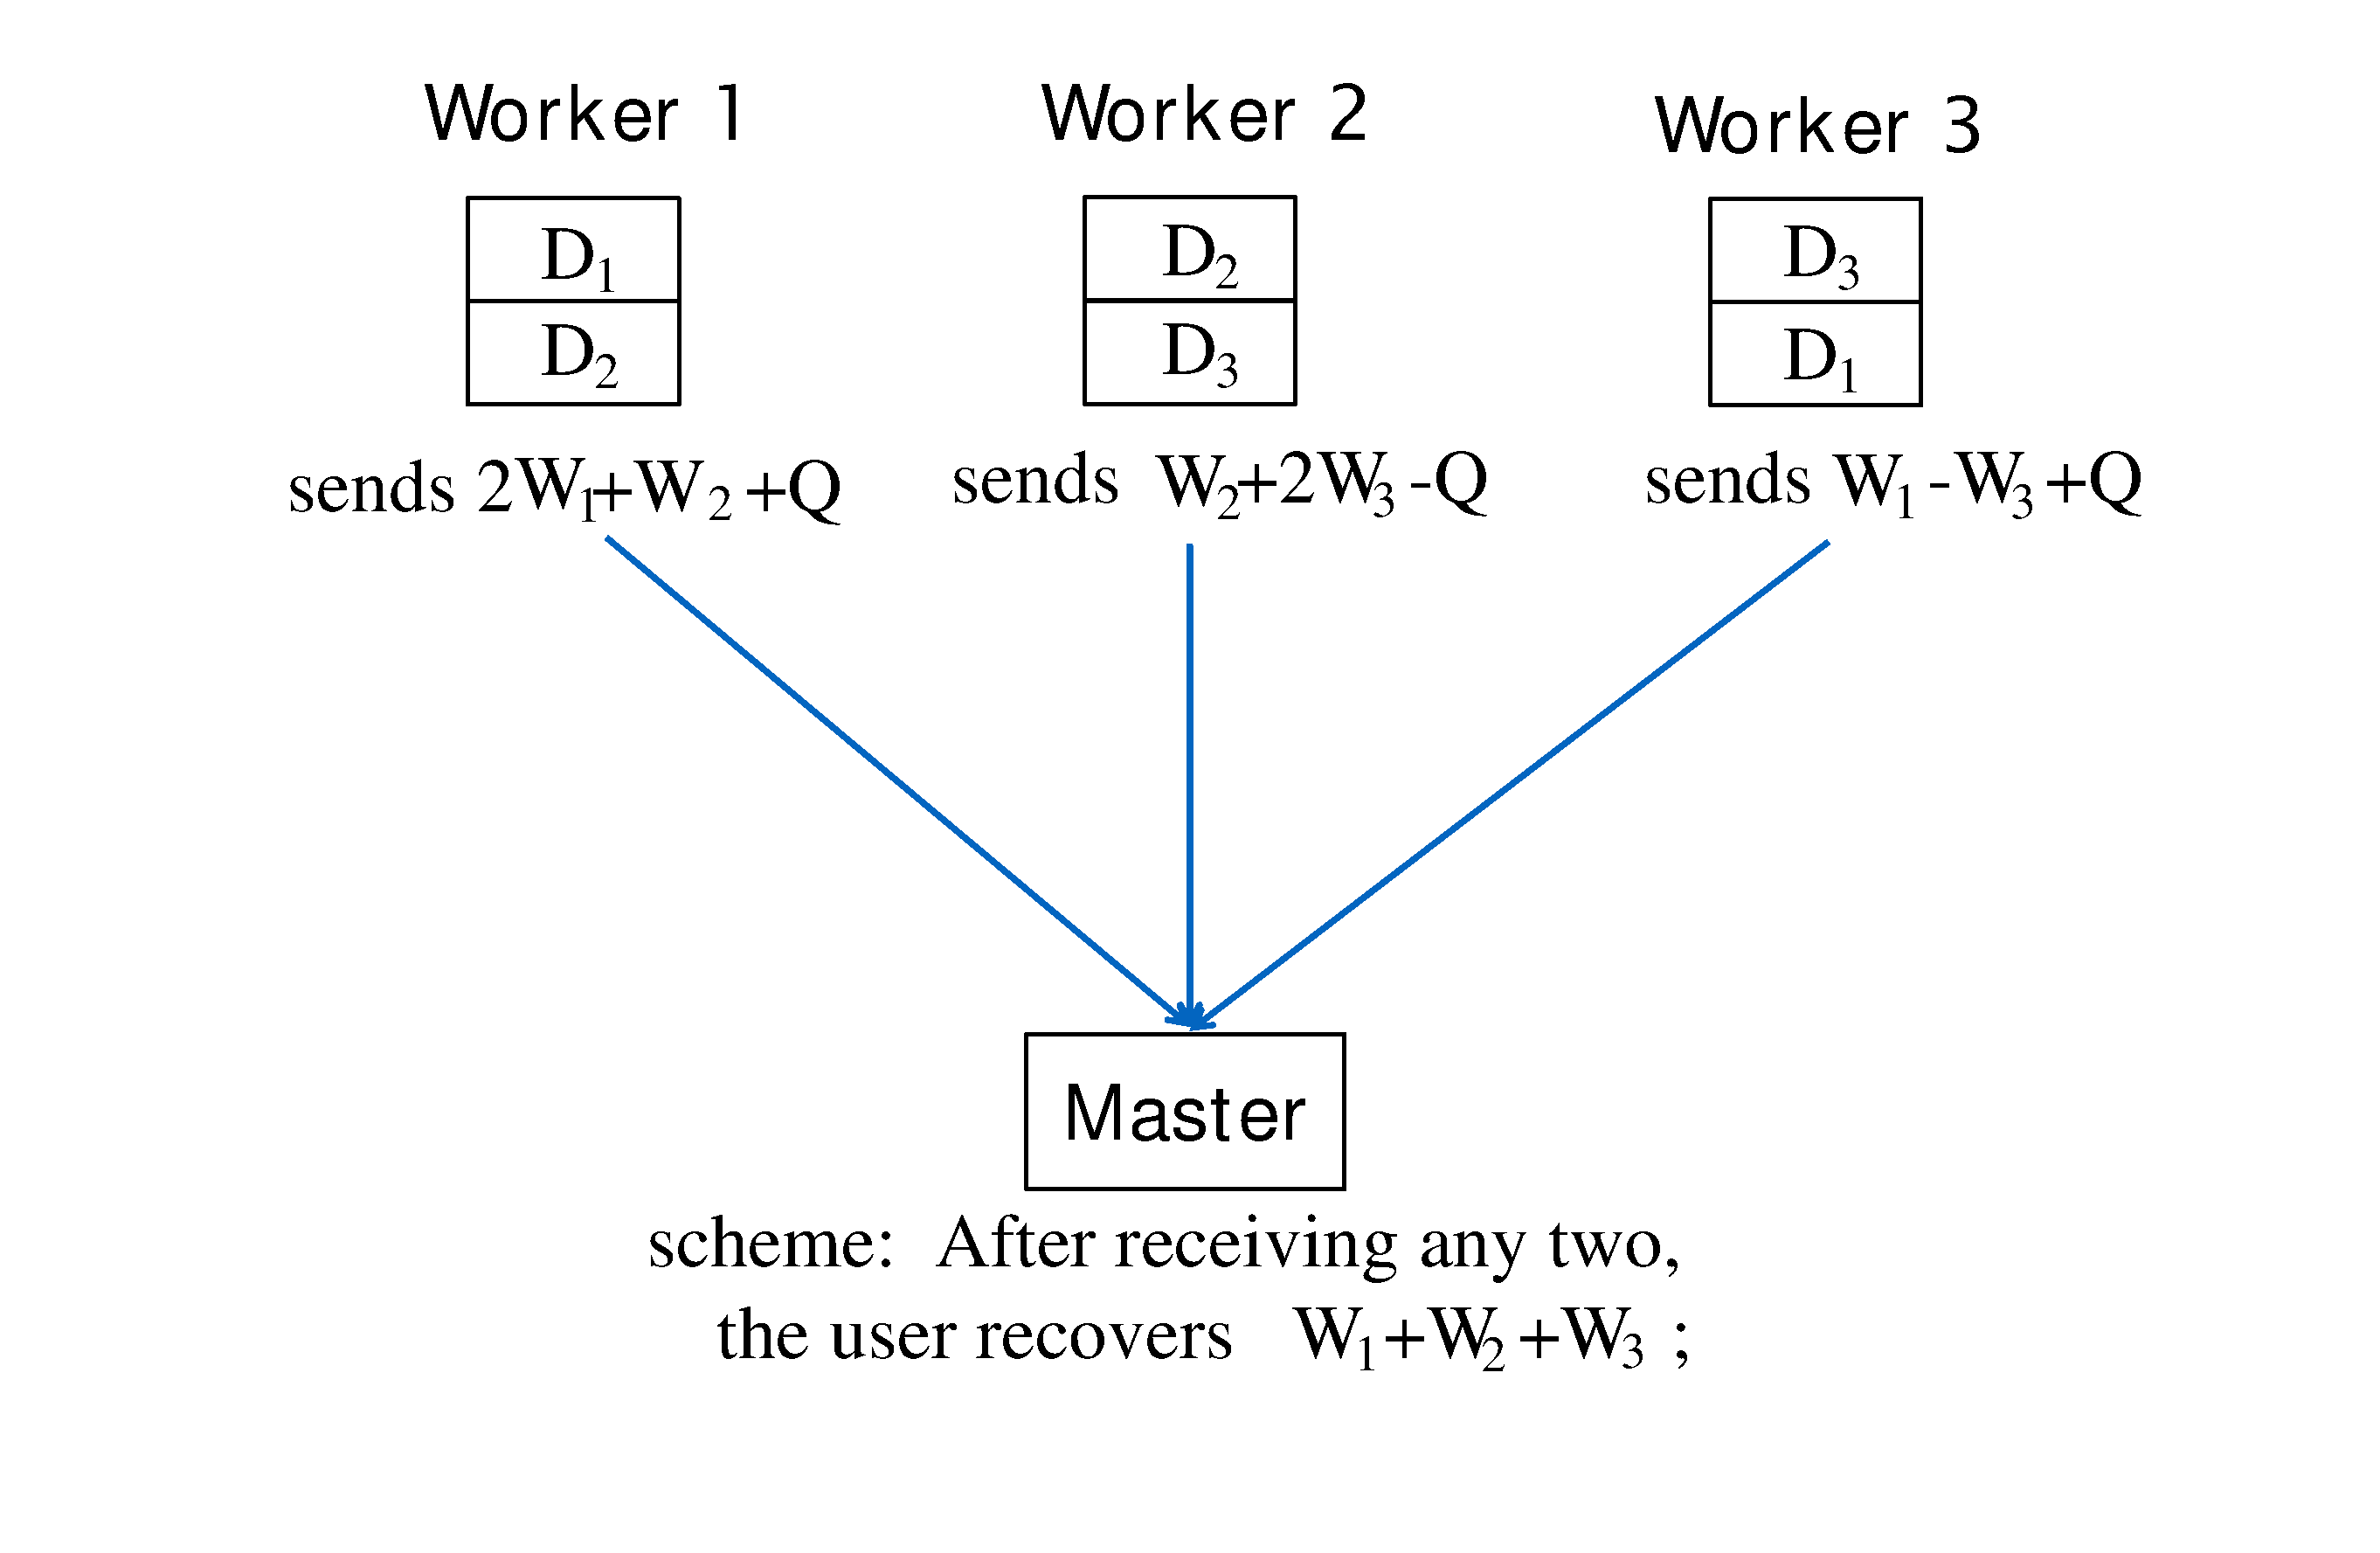
\includegraphics[scale=0.2]{secure_computation}}
\caption{\small $(\Ksf,\Nsf,\Nsf_{\rm r},\Ksf_{\rm c},\msf)=(3,3,2,1,1) $ secure distributed linearly separable  computation.}
\label{fig: system_model}
%\vspace{-5mm}
\end{figure}

Recently, the authors of \cite{wan2022secure} considered security constraints for the above problem, i.e., letting the master retrieve only the desired task function without obtaining any other information about the $\Ksf$ datasets. As shown in Fig. 1, where  $\Ksf=\Nsf=3$, $\Nsf_{\rm r}=2$, $\Ksf_{\rm c}=1$, $\Msf=2$, and the task function is $W_1+W_2+W_3$. To ensure security, in the data assignment phase, the data center uniformly generates a dataset-independent random key $Q $ over $[\mathbb{F}_{\qsf}]^{\Lsf}$ and assigns $Q $ to each worker. In the computing phase, each worker participates its obtained random key $Q $ in the encoding computation of the intermediate message. Worker $1$ computes $2W_1 + W_2 + Q$;   worker $2$ computes $W_2 + 2W_3 - Q$;   worker $3$ computes $W_1 - W_3 + Q$.In the decoding phase, from the answers of any two workers, the master can recover the task functions $W_1+W_2+W_3$.It can be seen that even if the master receives answers from all workers, it will not be able to obtain any other information about the dataset because $Q $ is unknown to it. Furthermore, it is stated in \cite{wan2022secure} that for any linear coding-based computation scheme, security can be guaranteed without increasing the communication cost.

\fi

\section{System Model}
\label{sec:system}

We consider the security aggregation of distributed linearly separable computation over the canonical master-worker distributed system, originally proposed in~\cite{wan2022secure}. 
A master wants to compute a function of $\Ksf$  datasets $D_1, \ldots, D_{\Ksf}$, with the help of $\Nsf$ workers without obtaining any other information about the input datasets. From any $\Nsf_{\rm r}$ workers' messages, the master can complete the computation task. Each worker is assigned $\Msf = \Nsf - \Nsf_{\rm r} + \msf$ datasets. 

With the assumption that the function is linearly separable from the datasets, the computation task can be written as $\Ksf_{\rm c}\leq \Ksf$ linear combinations of $\Ksf$ messages
\begin{align}
    &f({D_1},{D_2}, \ldots ,{D_{\Ksf}}) = g({f_1}({D_1}), \ldots ,{f_{\Ksf}}({D_{\Ksf}}))  \nonumber\\
    &= g({W_1}, \ldots ,{W_{\Ksf}}) = {\bf F}[{W_1}; \ldots ;{W_\Ksf}] = [{F_1};\ldots;{F_{\Ksf_{\rm c}}}], \label{eq:computation task}
\end{align}
where the $i^{\text{th}}$ message is  ${W_i} = {f_i}({D_i}) $, representing  the outcome of the  component function $f_i(\cdot)$ applied to dataset $D_i$. Each message $W_i$ contains $\Lsf$ uniformly i.i.d. symbols in $\mathbb{F}_{\qsf}$ for some large enough prime-power $\qsf$. ${\bf F}$ represents the demand matrix with dimension $\Ksf_{\rm c} \times \Ksf$, where each element is uniformly i.i.d. over $\mathbb{F}_{\qsf}$\footnote{\label{foot:L large}In this paper, we assume that  $\Ksf/\Nsf$ is an integer and  $\Lsf$ is large enough such
that any sub-message division is possible. We only consider $\Ksf_{\rm c} \leq \Ksf$ because when $\Ksf_{\rm c} \le \Ksf,$  $\text{Rank}({\bf F}) = \Ksf_{\rm c}$ with high probability and when $\Ksf_{\rm c} > \Ksf,$ $\text{Rank}({\bf F}) = \Ksf$ with high probability, we only consider the non-trivial setting $\Ksf_{\rm c} \le \Ksf$}. 

The secure aggregation scheme imposes the following conditions: 
\begin{align}
    I\big(W_{1},\ldots, W_{\Ksf};   X_{[\Nsf]} | {\bf F}   [W_1;\ldots;W_{\Ksf}]  \big)=0,
\end{align}
where $X_{[\Nsf]}$ presents the whole messages from $\Nsf$ workers.

Compared to distributed computing without considering secure aggregation, there is a trusted third-party server to ensure the security, which generates a set of dataset-independent random variables $\Qc = \{Q_{1}, \ldots, Q_{\Nsf}\}$ on $\mathbb{F}_{\qsf}$ and assigns them to workers based on indices. Notice that   
\begin{align}
I(Q_1, \ldots, Q_{\Nsf} ; D_1, \ldots, D_{\Ksf} )&=I(Q_1, \ldots, Q_{\Nsf} ; W_1, \ldots, W_{\Ksf} ) \nonumber\\ 
&=0. \label{eq:independent key}
\end{align}
The key size \( \eta \) measures the amount of randomness, i.e.,
\begin{align}
\eta = \frac{H( Q_1, \ldots, Q_{\Nsf} )}{\Lsf}, \label{eq:def of eta}
\end{align}


The distributed computing framework comprises three phases, {\it data assignment, computing, and decoding}. 

{\it Data assignment phase.}
We assign $\Msf:=\frac{\Ksf}{\Nsf} (\Nsf-\Nsf_{\rm r}+\msf)$ datasets to each worker. $\Zc_n$ denotes the set of indices of datasets assigned to worker $n$, where $\Zc_n \subseteq [\Ksf]$ and $|\Zc_n| \leq \Msf$. In addition, the third trusted server distributes the keys to each worker for security.

\iffalse
As an additional security restriction, we impose that the master learns no further information about $({D_1},\ldots,{D_{\Ksf}})$ other than the task function $f({D_1}, \ldots,{D_{\Ksf}})$.
To accomplish this, the third-party worker also generates a randomness variable $Q \in \Qc$ and assigns $Q $ to each worker  $k\in [\Ksf]$. Notice that   
\begin{align}
I(Q ; D_1, \ldots, D_{\Ksf} )=I(Q ; W_1, \ldots, W_{\Ksf} )=0. \label{eq:independent key}
\end{align}

The   randomness
size $\eta$ measures the   amount of   randomness, i.e.,
\begin{align}
\eta= \frac{H( Q_1, \ldots, Q_{\Nsf} )}{\Lsf}. \label{eq:def of eta}
\end{align}

However, in practice, each worker does not need to know all the keys, i.e., they do not need to store the full key size. Each worker only needs to store part of the key to achieve security, which we call individual key size, regardless of changes in the objective function.

\fi


{\it Computing phase.}
Each worker $n \in[\Nsf]$ first computes the message $W_k = f_k (D_k)$ for each $k \in \Zc_n$. Then it computes the coded message 
\begin{align}
 X_n = \psi_n \left( \{W_k:  k \in \Zc_n\},  Q \right),
 \end{align}
  where  $\psi_n$  is a  function of messages $\{W_k: k\in \Zc_n\}$, 
\begin{align} 
\psi_n &:  \mathbb{F}_{\qsf}^{ |\Zc_n| \Lsf} \times   | \Qc |  \to \mathbb{F}_{\qsf}^{ \Tsf_n },  
\label{eq: encoding function def}
\end{align}
and $\Tsf_n$ represents the length of $ X_n $. Finally, worker $n$ sends $X_n$ back to the master. $|\Zc_n|$ is denoted as the computation cost.\footnote{\label{computation cost} In a distributed system, the complexity of computing the linear combinations of the messages is much lower than computing the separable functions. So, the computation cost can be represented by the number of messages each worker computes.}


{\it Decoding phase.}
%To improve the effectiveness, 
%The master waits for the coded messages from the first $\Nsf_{\rm r}$ arriving workers. 
%for any pair of $\Nsf_{\rm r}$ active workers, 
The master can use coded messages from any $\Nsf_{\rm r}$ arriving workers to decode the computation tasks since the transmission environment and the computation capability of each worker are unknown. 
%The computing scheme should be designed to tolerate any $\Nsf - \Nsf_{\rm r}$ stragglers.
Thus, for each subset of workers $\Ac \subseteq [\Nsf]$ where $|\Ac| = \Nsf_{\rm r}$, by defining
$
    {X_{\Ac}}: = \{ {X_n}:n \in \Ac\}, 
$
there should be a decoding function such that 
$
\hat{g}_{\Ac}= \phi_{\Ac}\big( X_{\Ac}, {\bf F} \big),
$
where 
\begin{align}
    {\phi _\Ac}: \mathbb{F}_{\qsf}^{\sum_{n \in \Ac}{\Tsf_{\rm n}}} \times {\mathbb{F}_{\qsf}}^{{\Ksf_{\rm c}}\times \Ksf} \to {\mathbb{F}_{\qsf}}^{{\Ksf_{\rm c}}\times \Lsf}.
\end{align}
    

The  worst-case error probability is defined as
\begin{align}
 \varepsilon:= \max_{\Ac  \subseteq [\Nsf]: |\Ac|= \Nsf_{\rm r}} \Pr\{ \hat{g}_{\Ac} \neq g(W_1,   \ldots, W_{\Ksf}) \}. 
\end{align}
A computing scheme is called achievable if   the  worst-case     
error probability vanishes when $\qsf \to \infty$. 

We first introduce a novel converse bound on $ \eta $ for a fixed assignment, whose proof can be found in Appendix~\ref{sec:bound proof}.
\begin{thm}
\label{thm:bound of η}
For the $(\Ksf,\Nsf,\Nsf_{\rm r},\Ksf_{\rm c}, \msf)$ secure distributed linearly separable computation problem with  $\Msf= \frac{\Ksf}{\Nsf} (\Nsf - \Nsf_{\rm r} + \msf)=\frac{\Ksf}{\Nsf} \Msf^{\prime}$ and $\Ksf_{\rm c}=1$, for a fixed assignment $\mathbf{Z}=(\Zc_1,\ldots,\Zc_{\Nsf})$, if there  exists an ordered set of workers in $[\Nsf]$ denoted by $\sv =(s_1,\ldots,s_{|\sv| })$, 
\begin{align}
\forall i \in [|\sv|], \exists x \in \Zc_{s_i} \text{ such that } \sum_{j=1}^{i-1} \mathbb{1}(x \in \Zc_{s_j}) \le m-1, \label{eq:vector constraint}
\end{align}
where the symbol \(\mathbb{1}(A)\) denotes the indicator function, which is \(1\) if the condition \(A\) is true, and \(0\) otherwise.
It must hold that
\begin{align}
\eta \geq \frac{|\sv|}{\msf}-1. \label{eq:converse lemma}
\end{align}
\end{thm}
 \begin{cor}
\label{cor:converse cor}
For the $(\Ksf,\Nsf,\Nsf_{\rm r},\Ksf_{\rm c}, \msf)$ secure distributed linearly separable computation problem with  $\Msf= \frac{\Ksf}{\Nsf} (\Nsf - \Nsf_{\rm r} + \msf)=\frac{\Ksf}{\Nsf} \Msf^{\prime}$ and $\Ksf_{\rm c}=1$,
% to achieve the optimal communication cost, 
 it must hold that
\begin{align}
\eta^{\star} \geq \frac{\left\lceil  \frac{\msf\Nsf}{\Nsf-\Nsf_{\rm r}+1} \right\rceil}{\msf} -1. \label{eq:converse cor}
\end{align}
\end{cor} 
It can be seen that the key size $ \eta $ depends on the data assignment.
In this paper, we discuss %the following two system parameters:
%\begin{itemize}
  the minimum $\eta^{*}$ required for the secure aggregation of distributed linearly separable computation.
   % \item The minimum individual key size \( \Qsf^{*}_{\rm s} \) for unknown demand.%$\min\limits_{\forall n \in [\Nsf]} H(Q^{*}_n)$ . 
%\end{itemize}

Notice that in order to satisfy security constraints, it should satisfy that
 \begin{align}
I\big(W_{1},\ldots, W_{\Ksf};   X_{[\Nsf]} | {\bf F}   [W_1;\ldots;W_{\Ksf}]  \big)=0. 
\end{align}

We define 
\begin{equation}
    \Rsf: = \mathop {\max }\limits_{\Ac \subseteq [\Nsf]:|\Ac| = {\Nsf_{\rm r}}} \frac{{\sum\nolimits_{n \in \Ac} {{\Tsf_n}} }}{\Lsf}
\end{equation} 
as the communication cost, 
which represents the maximum normalized number of symbols received from any $\Nsf_{\rm r}$ workers to recover the computational task.

In this paper, we focus on the minimum key size under the optimal communication cost, when $\Ksf_{\rm c} = 1, \msf \geq 1$.

\section{Main Results}
\label{sec:main}


\iffalse
For ease of analysis, we only consider $\Ksf = \Nsf$ in the following.~\footnote{We consider the situation that $\Ksf$ datasets can be partitioned into $\Nsf$ non-overlapping groups of equal length. {\red virtual datasets}. Specifically, the $i^{\text{th}}$ group, denoted as $\Gc_i = \{k \in [\Ksf]: \text{Mod}(k,\Nsf) = i\}$, contains $\frac{\Ksf}{\Nsf}$ datasets, for each $i \in [\Nsf]$. Each group $\Gc_i$ is then assigned to $\Msf^{\prime} = \Nsf - \Nsf_{\rm r} + \msf$ workers, where these workers collaboratively compute the merged message $W^{\prime}_i$.} 

we can thus reformulate the $(\Ksf, \Nsf, \Nsf_{\rm r}, \Ksf_{\rm c}, \Msf)$ secure distributed linearly separable computation problem as an equivalent $(\Nsf, \Nsf, \Nsf_{\rm r}, \Ksf_{\rm c}, \Msf^{\prime})$ problem in the following discussion.
\fi

\begin{thm}
\label{thm:main achievable scheme}
For the $(\Ksf,\Nsf,\Nsf_{\rm r},\Ksf_{\rm c}, \msf)$ secure distributed linearly separable computation problem with  $\Msf= \frac{\Ksf}{\Nsf} (\Nsf - \Nsf_{\rm r} + \msf)=\frac{\Ksf}{\Nsf} \Msf^{\prime}$ and $\Ksf_{\rm c}=1$, the optimal key size  $\eta=  \frac{ h(\Nsf,\Msf^{\prime})}{\msf}-1$ is achievable, where the output of the function \( h(\cdot, \cdot) \) is given by the recursive algorithm shown in Fig.~\ref{fig:scheme} with the following properties:
 \begin{itemize}

 \item When  $\Nsf > 2\Msf^{\prime}$,  by {\it Scheme~1} described in Section~\ref{sub:partial rep} we have  
\begin{align}
h(\Nsf,\Msf^{\prime})=h\big(\Nsf-\left\lfloor \Nsf/\Msf^{\prime}-1\right\rfloor \Msf^{\prime},\Msf^{\prime}\big)+ \msf\left\lfloor \Nsf/\Msf^{\prime} -1\right\rfloor  . \label{eq:from partial rep}
\end{align} 
\item When $1.5 \Msf^{\prime} \leq \Nsf < 2 \Msf^{\prime}$ and $\Msf^{\prime}$ is even, with $\Msf^{\prime} \geq 2\msf$,
by {\it Scheme~2} described in Section~\ref{sub:M is even}, we have  
\begin{align}
 h(\Nsf, \Msf^{\prime}) = h\left(\Nsf - \Msf^{\prime}, \frac{\Msf^{\prime}}{2}\right) + \msf. \label{eq:M is even}
\end{align}

 \item When $1.5 \Msf^{\prime} \leq  \Nsf < 2 \Msf^{\prime}$ and $\Msf^{\prime}$ is odd, with $\Msf^{\prime} \geq 2\msf+1$, by  {\it Scheme~3} described in Section~\ref{sub:M is odd} we have  
 \begin{align}
 h(\Nsf,\Msf^{\prime})=   \Nsf-\frac{3\Msf^{\prime}-1}{2}+2 \msf; \label{eq:M is odd}
 \end{align}
 \item When $\Msf^{\prime}< \Nsf <  1.5 \Msf^{\prime}$, with $\Msf^{\prime} \geq 2\msf$, by  {\it Scheme~4} described in Section~\ref{sub:less than 1.5M}  we have  
\begin{align}
h(\Nsf,\Msf^{\prime})=h(\Msf^{\prime},2\Msf^{\prime}-\Nsf). \label{eq:less than 1.5M}
\end{align} 
  \end{itemize}
    \hfill $\square$ 
 \end{thm} 
Notice that $\lambda$ in Fig.~\ref{fig:scheme} represents the number of totally transmitted linearly independent combinations of merged messages, and we aim to minimize it.
 
\begin{rem}[The key size in extreme cases]
\label{rem:extreme cases}
\em

For the $(\Ksf, \Nsf, \Nsf_{\rm r}, \Ksf_{\rm c}, \msf)$ secure distributed linearly separable computation problem, where $\Msf = \frac{\Ksf}{\Nsf} (\Nsf - \Nsf_{\rm r} + \msf) = \frac{\Ksf}{\Nsf} \Msf^{\prime}$, $\Ksf_{\rm c} = 1$, and $\Msf$ divides $\Nsf$, the minimum required key size to achieve the optimal communication cost is
\begin{align}
    \eta^{\star} = \frac{\Nsf}{\Msf^{\prime}} - 1. \label{eq:gradient eta rho rep}
\end{align}

For the $(\Ksf, \Nsf, \Nsf_{\rm r}, \Ksf_{\rm c}, \msf)$ secure distributed linearly separable computation problem, where $\Msf = \frac{\Ksf}{\Nsf} (\Nsf - \Nsf_{\rm r} + \msf)$ and $\Ksf_{\rm c} = 1$, the minimum key size required to achieve the optimal communication cost, under the cyclic assignment constraint, is given by
\begin{align}
    \eta^{\star}_{\text{cyc}} = \frac{\Nsf_{\rm r}}{\msf} - 1. \label{eq:gradient eta cyc}
\end{align}

\end{rem}

\begin{rem}[Simplification of the security problem]
\label{rem:no secure}
\em
As shown in~\cite[Theorem 2]{wan2022secure}, for any $(\Ksf, \Nsf, \Nsf_{\rm r}, \Ksf_{\rm c}, \msf)$ non-secure distributed linearly separable computation problem, the encoding scheme can be made secure without increasing the communication cost. Therefore, for the secure distributed linearly separable computation problem, we can simplify the problem to the encoding schemes of non-secure distributed linearly separable computation, corresponding to the scheme we propose later in this work.
\end{rem}
At the end of this section, we present numerical evaluations comparing the key size required by the cyclic assignment scheme and the combined scheme from Theorem~\ref{thm:main achievable scheme}, both achieving optimal communication cost. In Fig.~\ref{fig:numerical 1a}, we fix $\Nsf = 24, \msf = 2$ and show the tradeoff between $\Msf$ and $\eta$. In Fig.~\ref{fig:numerical 1b}, we fix $\Msf = 6, \msf = 2$ and show the tradeoff between $\Nsf$ and $\eta$. In Fig.~\ref{fig:numerical 1c}, we fix $\Nsf = 24, \Msf = 10$ and show the tradeoff between $\msf$ and $\eta$. The results demonstrate that the combined scheme requires a significantly smaller key size than the cyclic assignment scheme.


\begin{figure*}%[ht]
%\vspace{-2mm}
\centerline{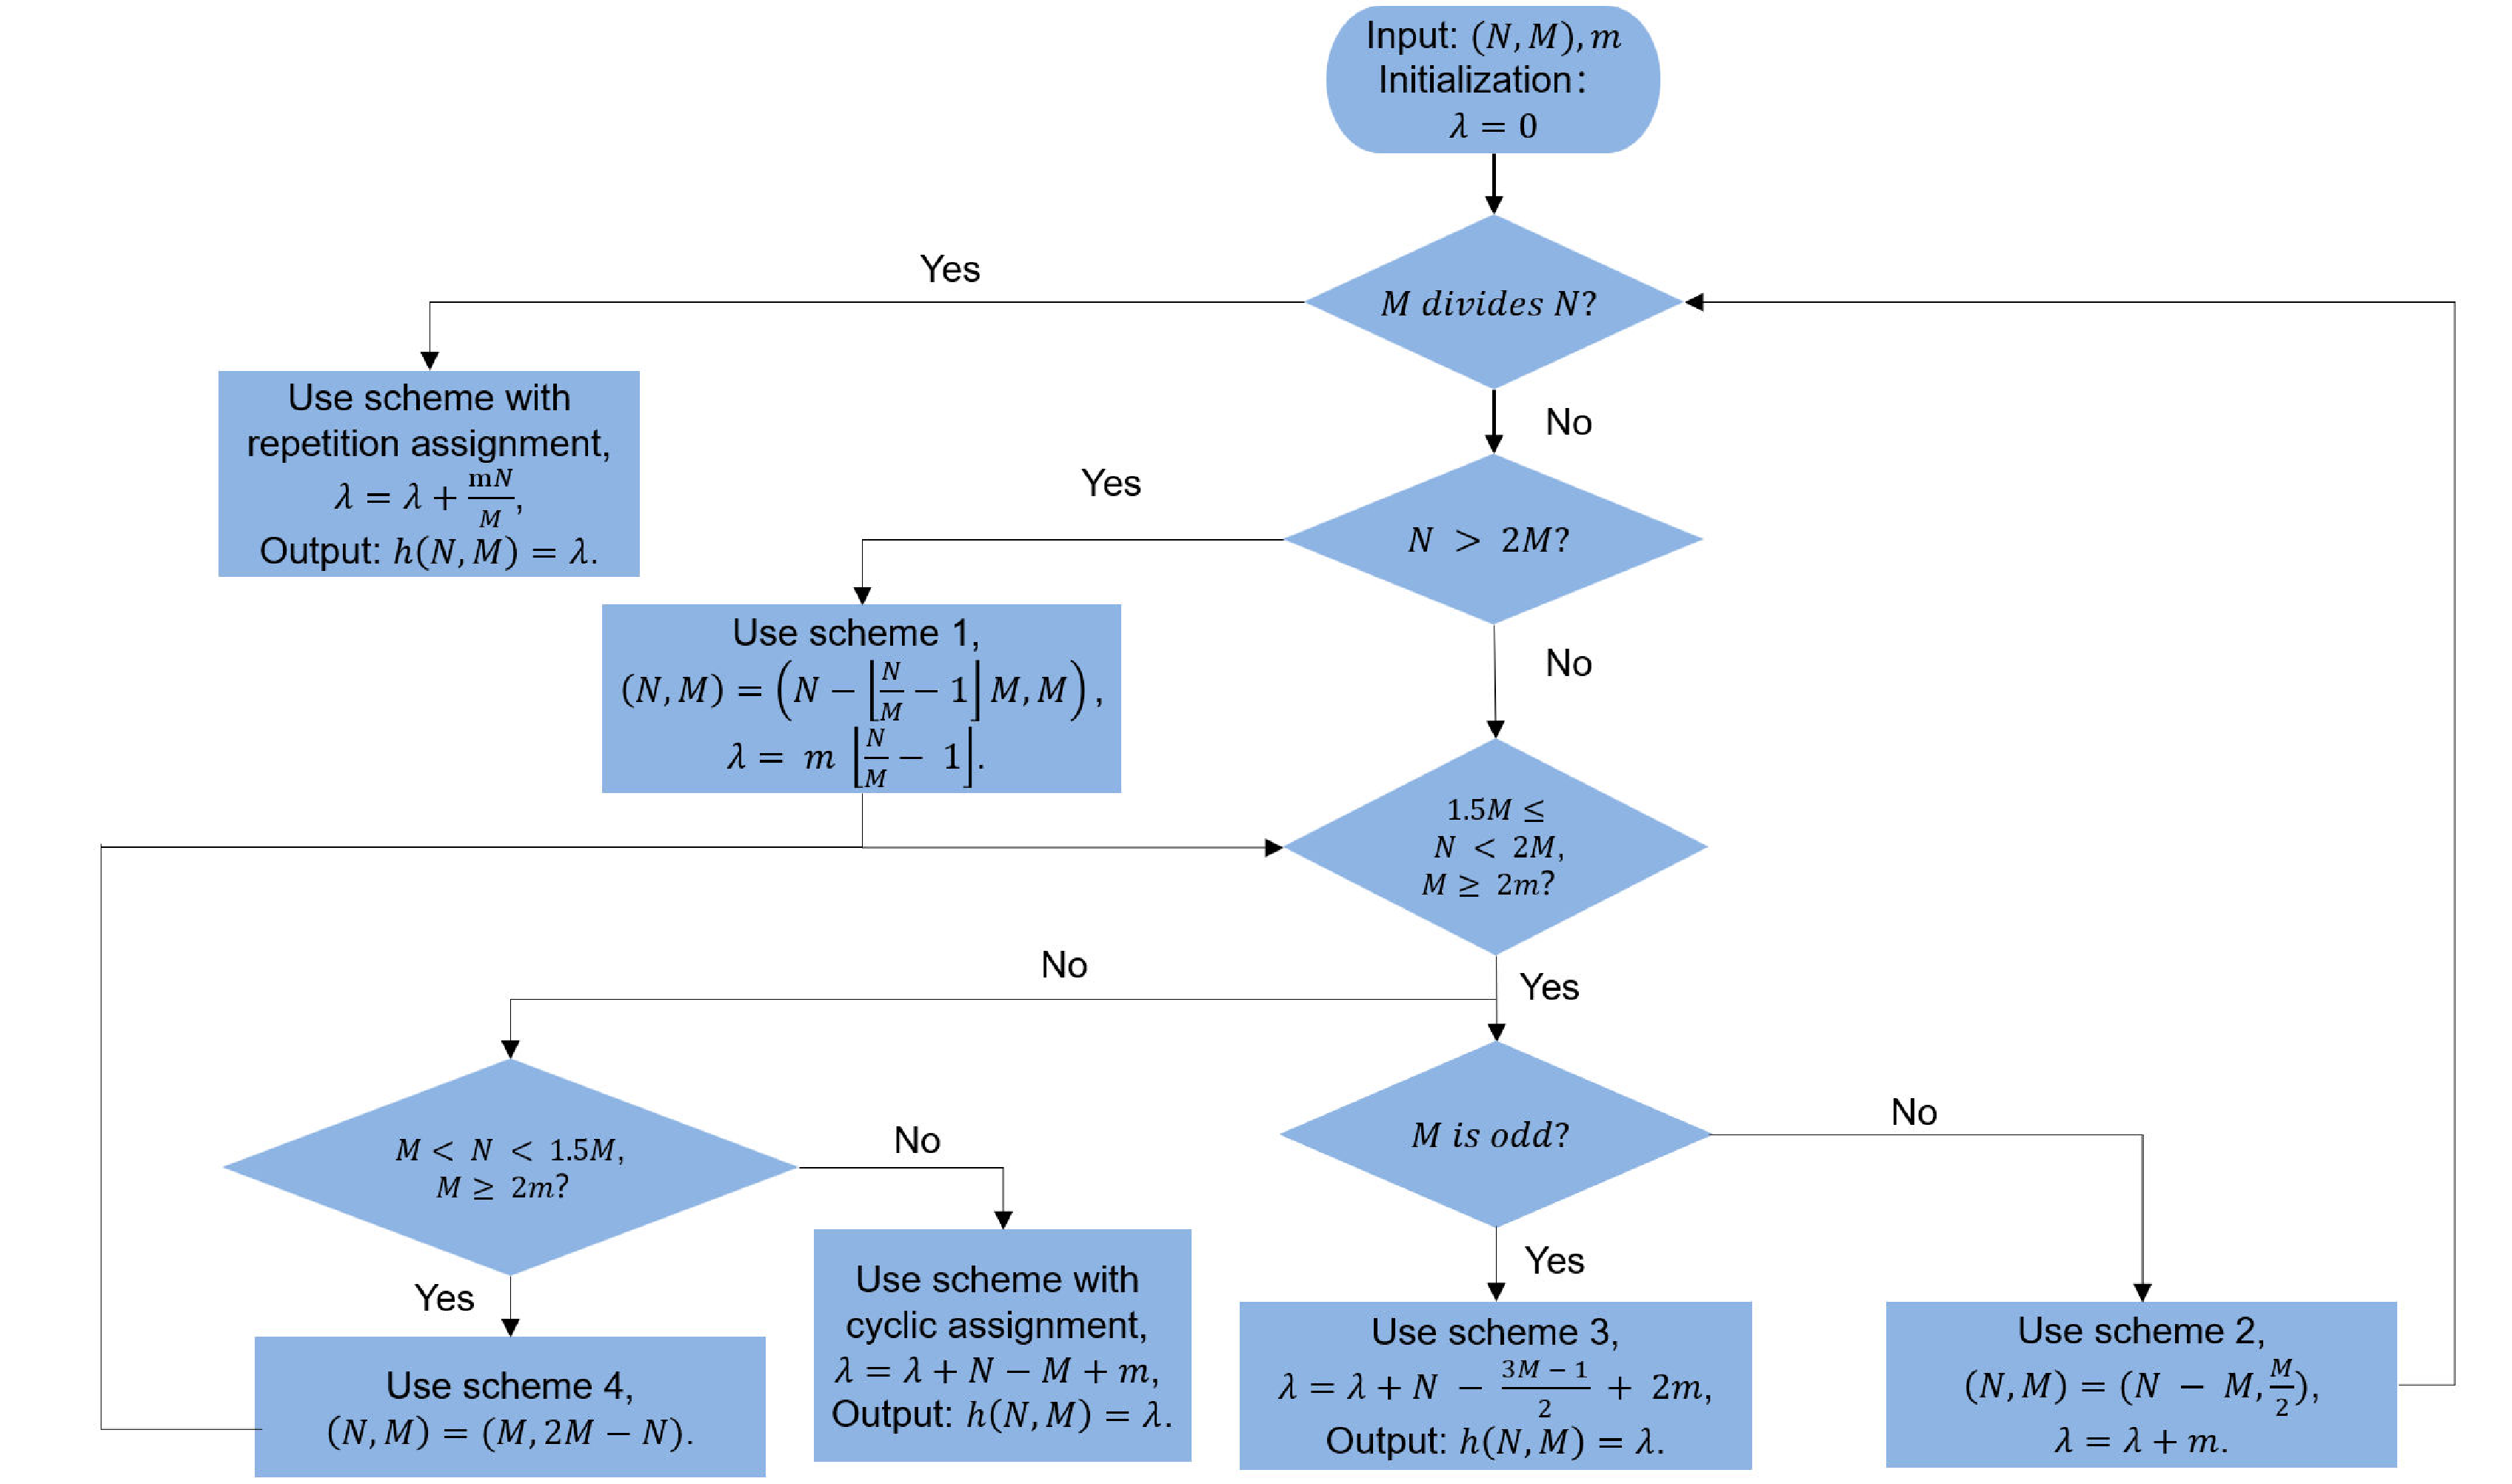
\includegraphics[scale=0.3]{scheme}}
\caption{\small Flow diagram of the combined scheme in Theorem~\ref{thm:main achievable scheme}.}
\label{fig:scheme}
\rule{\textwidth}{0.2pt} % 创建分割线
%\vspace{-5mm}
\end{figure*}


\begin{figure}[ht] 
    \centering
    \begin{subfigure}[t]{0.5\textwidth}
        \centering
        \includegraphics[scale=0.5]{M varies.pdf}
        \caption{\small $(\Msf,\eta)$ tradeoff with $\Nsf=24$ and $\msf=2$.}
        \label{fig:numerical 1a}
    \end{subfigure}\\
    \begin{subfigure}[t]{0.5\textwidth}
        \centering
        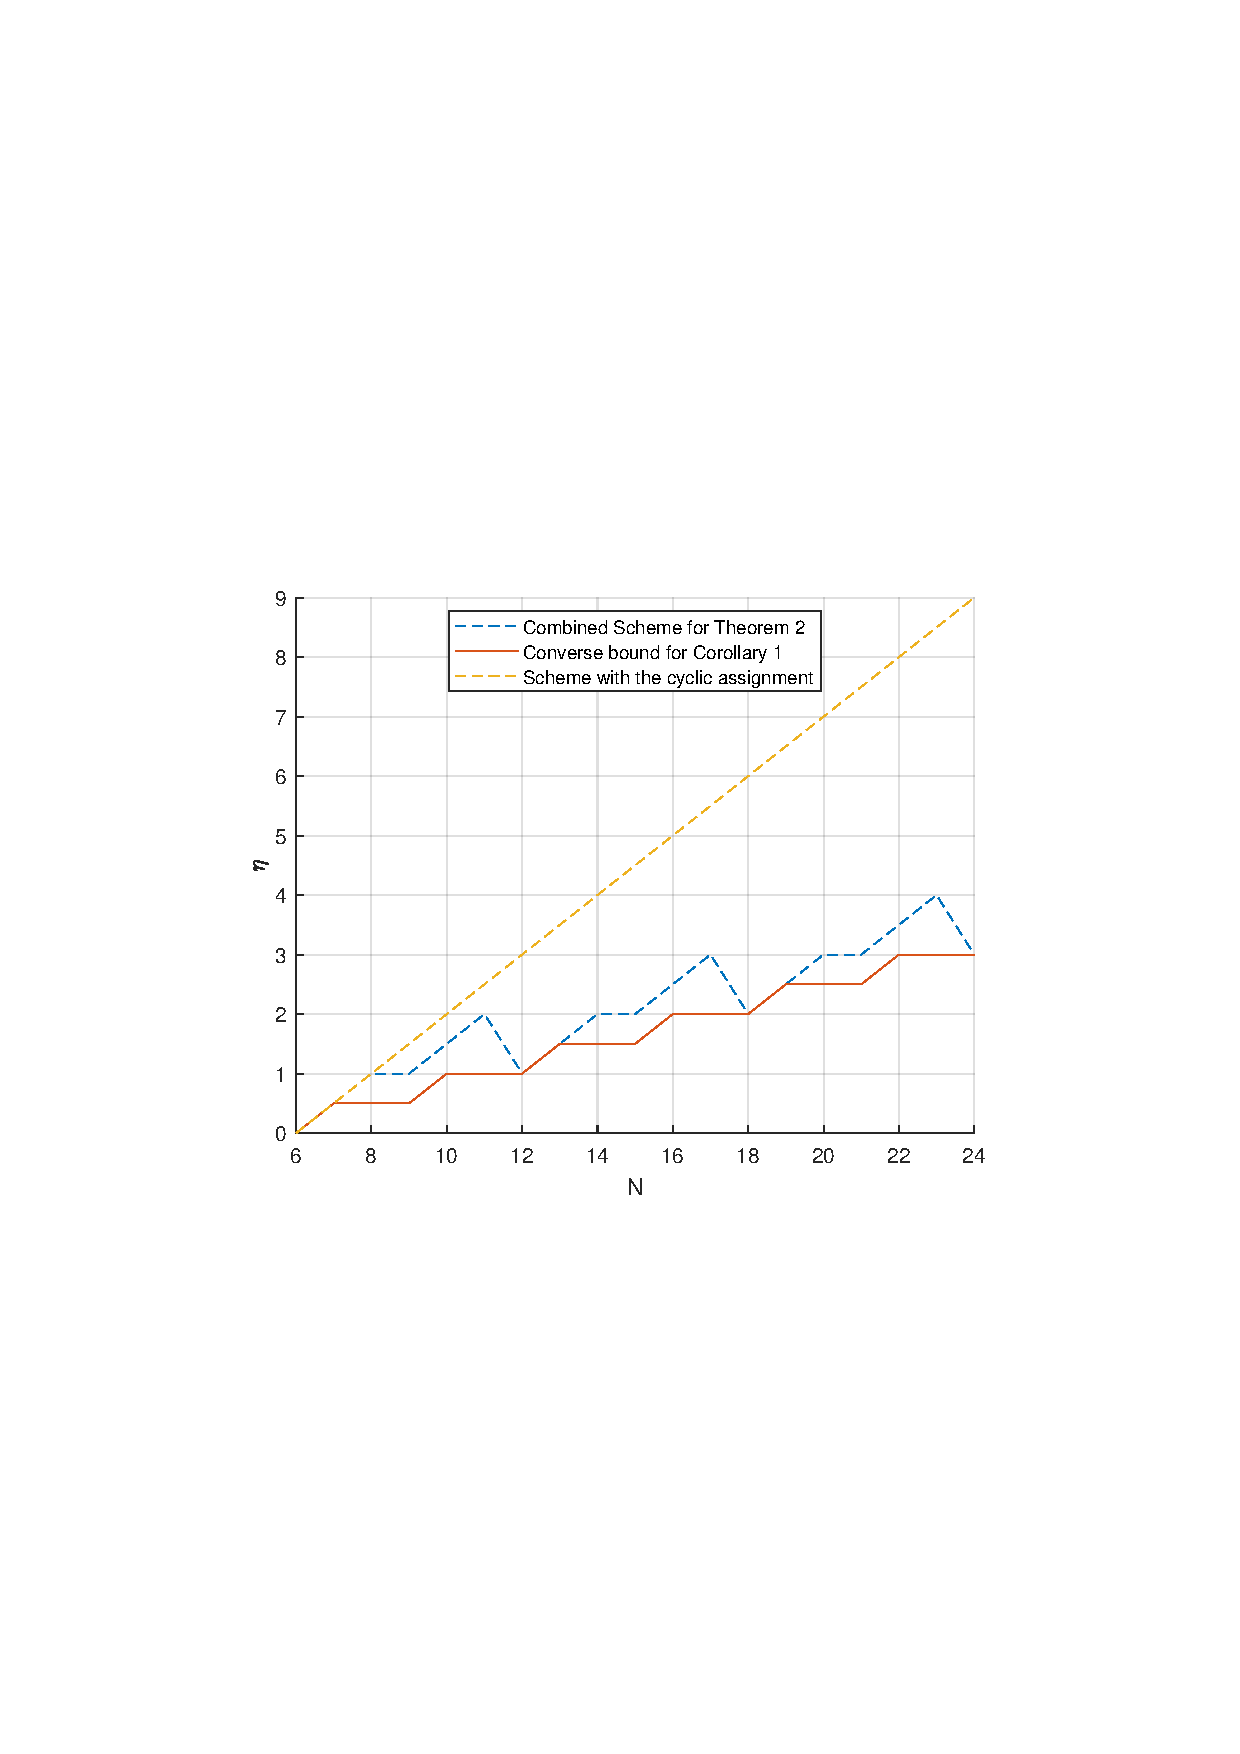
\includegraphics[scale=0.5]{N varies.pdf}
        \caption{\small $(\Nsf,\eta)$ tradeoff with $\Msf=6$ and $\msf=2$.}
        \label{fig:numerical 1b}
    \end{subfigure}\\
    \begin{subfigure}[t]{0.5\textwidth}
        \centering
        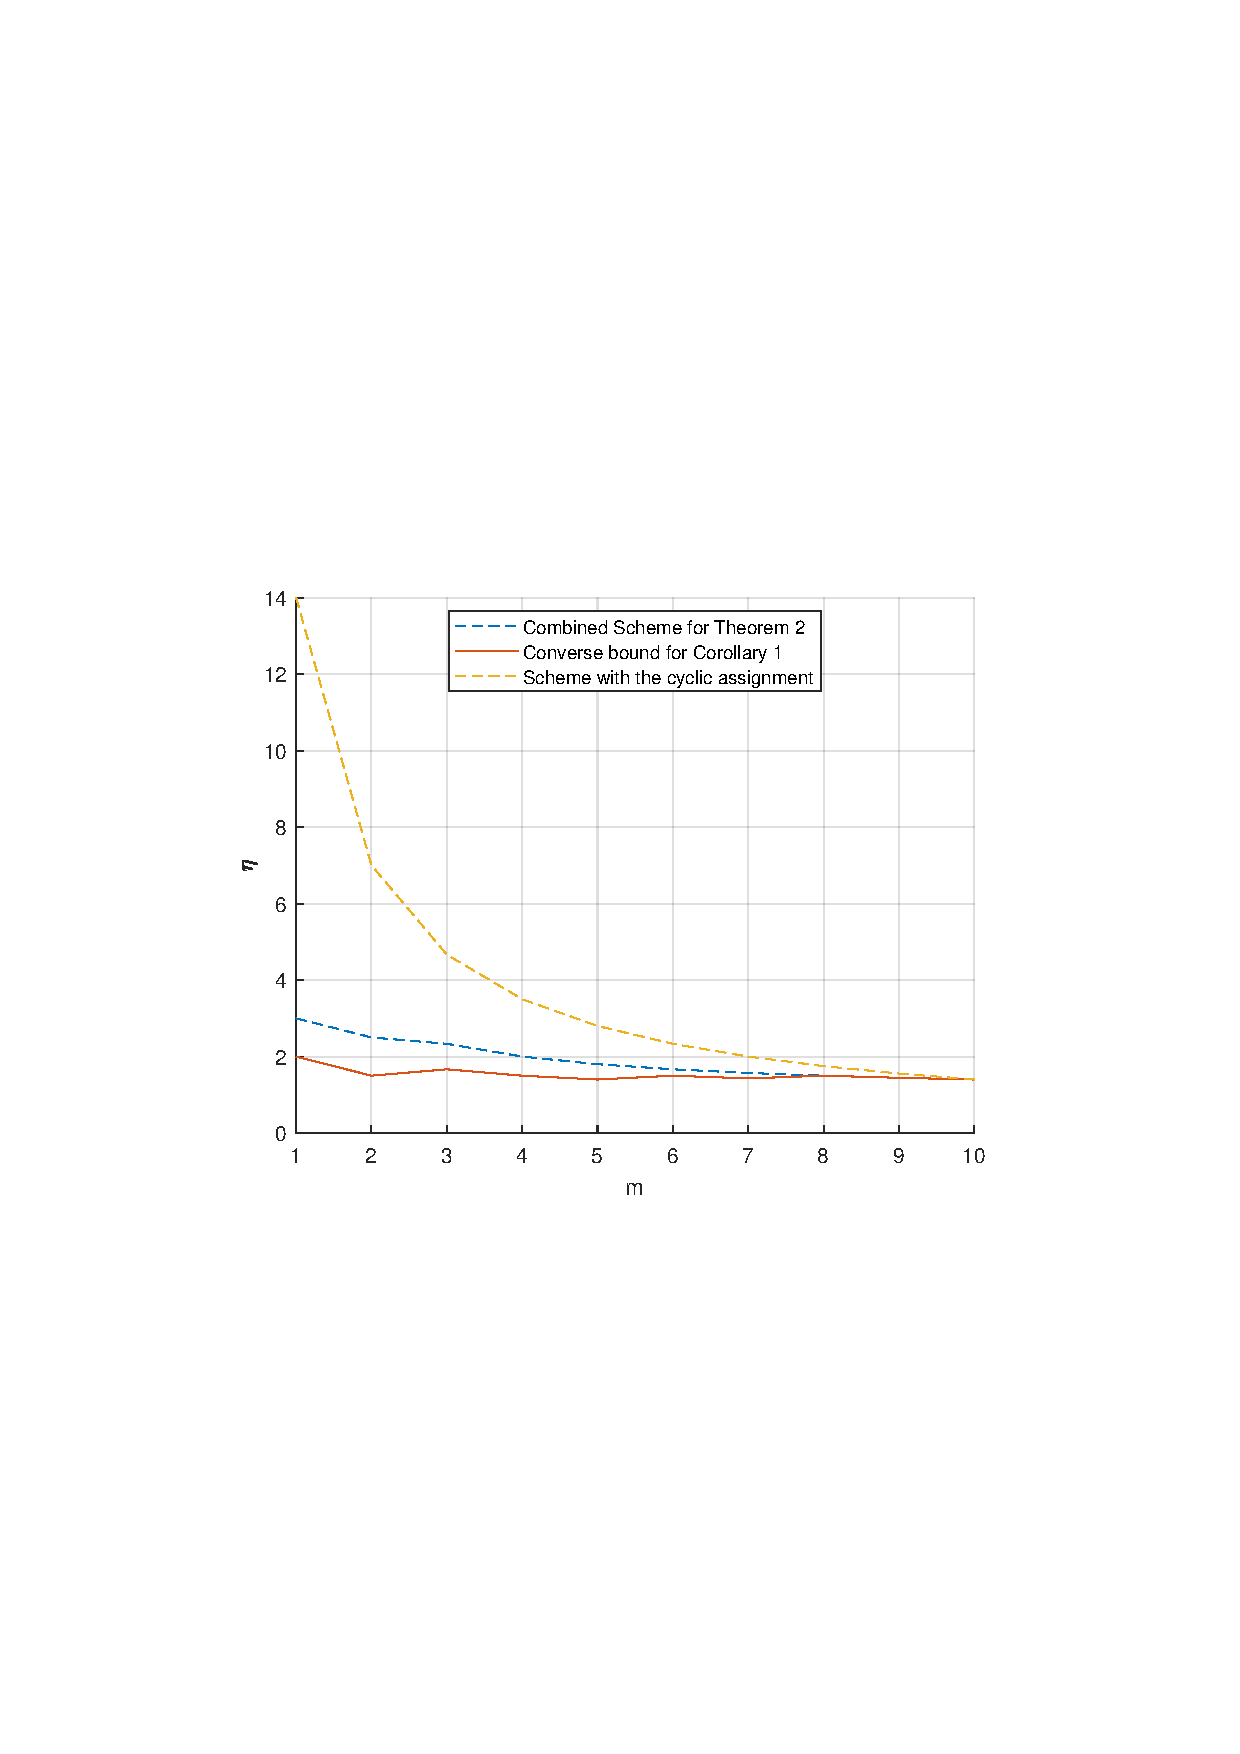
\includegraphics[scale=0.5]{m varies.pdf}
        \caption{\small $(\msf,\eta)$ tradeoff with $\Nsf=24$ and $\Msf=10$.}
        \label{fig:numerical 1c}
    \end{subfigure}
    \caption{\small Numerical evaluations for the considered secure distributed linearly separable computation problem.}
    \label{fig:numerical 1}
\end{figure}


\section{Novel Achievable Scheme For Theorem~\ref{thm:main achievable scheme}}
\label{sec:Achievable coding scheme}


\subsection{\texorpdfstring{Scheme~1 for~\eqref{eq:from partial rep}}{Scheme 1 for Eq. (X)}}
\label{sub:partial rep}
In this section, we consider the case where $\Nsf > 2\Msf$. We first focus on the workers and datasets in the range $[(i-1)\Msf+1: i\Msf]$ for any $i \in \left[\left\lfloor \Nsf/\Msf -1 \right\rfloor\right]$. The datasets in this range are assigned to the corresponding workers using the fractional repetition assignment strategy. This results in $\msf \left\lfloor \Nsf/\Msf -1 \right\rfloor$ linearly independent combinations of messages.

We then consider the remaining $\Nsf - \left\lfloor \Nsf/\Msf -1 \right\rfloor \Msf$ datasets and workers. The original $(\Nsf, \Msf)$ problem is thus reduced to solving a smaller problem of $(\Nsf - \left\lfloor \Nsf/\Msf -1 \right\rfloor \Msf, \Msf)$. The specific scheme for addressing this reduced problem is detailed below.

\begin{example}\rm
 \label{ex:7,3}   
We consider the $(\Nsf, \Msf) = (7, 3)$ non-secure problem, and assume $\msf = 2$, which gives $\Nsf_{\rm r} = \Nsf - \Msf + \msf = 6$.
For the sake of simplicity, we assume in this example that the field is a sufficiently large prime field;  in general, the proposed scheme does not need this assumption (recall that we only need the field size to be large enough). 

{\it Data assignment phase.}
The data assignment is shown in the following figure.
\begin{align*}
\begin{array}{rl|c|c|c|c|}\cline{3-3}\cline{4-4}\cline{5-5}\cline{6-6}
&&\rule{0pt}{1.2em}\mbox{Worker 1} & \rule{0pt}{1.2em}\mbox{Worker 2} &  \rule{0pt}{1.2em}\mbox{Worker 3}&  \rule{0pt}{1.2em}\mbox{Worker 4}  \\ \cline{3-3}\cline{4-4}\cline{5-5}\cline{6-6}
&& D_1 & D_1 & D_1 & D_4  \\
&& D_2 & D_2 & D_2 & D_5  \\
&& D_3 & D_3 & D_3 & D_6  \\ \cline{3-3}\cline{4-4}\cline{5-5}\cline{6-6}
\end{array}
\end{align*}

\begin{align*}
\begin{array}{rl|c|c|c|}\cline{3-3}\cline{4-4}\cline{5-5}
&&\rule{0pt}{1.2em}\mbox{Worker 5} &  \rule{0pt}{1.2em}\mbox{Worker 6} &  \rule{0pt}{1.2em}\mbox{Worker 7}  \\ \cline{3-3}\cline{4-4}\cline{5-5}
&&  D_5 & D_6 & D_7 \\
&&  D_6 & D_7 & D_4 \\
&&  D_7 & D_4 & D_5 \\ \cline{3-3}\cline{4-4}\cline{5-5}
\end{array}
\end{align*}


% For the sake of simplicity, we assume in this example that the field is a sufficiently large prime field; in general, the proposed scheme does not require this assumption (recall that we only need the field size to be large enough). 



{\it Computing phase.}
To achieve the optimal communication cost, we first divide each message $W_k, k \in [\Ksf]$, into $\msf$ non-overlapping and equal-length sub-messages, denoted as $W_{k} = \{W_{k,j} : j \in [\msf]\}$, so that each sub-message contains $\frac{\Lsf}{\msf} = \frac{\Lsf}{2}$ symbols in $\mathbb{F}_{\qsf}$.

After dividing the messages, we first have workers 1, 2, and 3, which store the same data, compute random linear combinations of $(W_{1,1} + W_{2,1} + W_{3,1})$ and $(W_{1,2} + W_{2,2} + W_{3,2})$. Specifically, we can assign the following computations:
 Worker 1 computes $W_{1,1} + W_{2,1} + W_{3,1} + W_{1,2} + W_{2,2} + W_{3,2}$,
 Worker 2 computes $W_{1,1} + W_{2,1} + W_{3,1} + 2(W_{1,2} + W_{2,2} + W_{3,2})$,
 Worker 3 computes $W_{1,1} + W_{2,1} + W_{3,1} + 3(W_{1,2} + W_{2,2} + W_{3,2})$.

  Next, we focus on workers 4, 5, 6, and 7. We use the cyclic assignment scheme to distribute data blocks $D_4, D_5, D_6$, and $D_7$ among these workers. According to the cyclic coding scheme, the computations are assigned as follows:
 Worker 4 computes $\frac{1}{2}W_{5,1} - W_{4,2} - \frac{2}{3}W_{6,2}$,
 Worker 5 computes $\frac{1}{2}W_{5,1} + W_{5,2} + \frac{1}{3}W_{6,2} + W_{7,2}$,
 Worker 6 computes $W_{4,1} + W_{6,1} + W_{7,1} + 2W_{4,2} + \frac{4}{3}W_{6,2}$,
 Worker 7 computes $\frac{3}{2}W_{5,1} - W_{4,2} + 2W_{5,2} + 2W_{7,2}$.


{\it Decoding phase.}
 Among the information received from any $\Nsf_{\rm r} = 6$ workers, at least two messages come from workers 1, 2, and 3. This allows the master to recover $W_{1,1} + W_{2,1} + W_{3,1}$ and $W_{1,2} + W_{2,2} + W_{3,2}$. Additionally, three messages are from workers 4, 5, 6, and 7, enabling the master to reconstruct $W_{4,1} + W_{5,1} + W_{6,1} + W_{7,1}$ and $W_{4,2} + W_{5,2} + W_{6,2} + W_{7,2}$. Together with the previously recovered information, the master can obtain $W_{1,1} + W_{2,1} + W_{3,1} + W_{4,1} + W_{5,1} + W_{6,1} + W_{7,1}$ and $W_{1,2} + W_{2,2} + W_{3,2} + W_{4,2} + W_{5,2} + W_{6,2} + W_{7,2}$.

It can be observed that the number of linearly independent combinations received from workers 1, 2, and 3 is 2, and from workers 4, 5, 6, and 7, the number of linearly independent combinations is 3. The total sum gives $h(7, 3) = 5$, which equals $h(4, 3) + \msf$ for $\msf = 2$, and this satisfies ~\eqref{eq:from partial rep}.

 Then we consider the general case of the $(\Nsf, \Msf)$ non-secure problem when $\Nsf > 2\Msf$, and provide a generic scheme for this case to prove ~\eqref{eq:from partial rep}. We assume that for the non-secure problem $\big(\Nsf - \left\lfloor \Nsf/\Msf - 1 \right\rfloor \Msf, \Msf\big)$, a specific scheme is already available, and from that scheme, we have obtained $h\big(\Nsf - \left\lfloor \Nsf/\Msf - 1 \right\rfloor \Msf, \Msf\big)$ linearly independent combinations.

\end{example}
{\it Data assignment phase.}
We partition the entire system into $\left\lfloor  \Nsf/\Msf \right\rfloor $ blocks. For each $i \in [\left\lfloor \Nsf/\Msf \right\rfloor - 1]$, the $i^{\text{th}}$ block includes the datasets $\{ D_{k}: k \in \left[(i-1)\Msf+1: i\Msf \right]\}$ and the workers in the range $\left[(i-1)\Msf+1: i\Msf \right]$.
The last block includes the datasets and workers in the range $\left[\left\lfloor \Nsf/\Msf - 1 \right\rfloor \Msf + 1 : \Nsf \right]$.

For the first $\left[\left\lfloor \Nsf/\Msf \right\rfloor - 1\right]$ blocks, we use the fractional repetition assignment to distribute the data. As for the last block, it contains $\Nsf - \left\lfloor \Nsf/\Msf - 1 \right\rfloor \Msf$ workers and $\Nsf - \left\lfloor \Nsf/\Msf - 1 \right\rfloor \Msf$ datasets, with each worker being able to compute $M$ datasets. Therefore, we can directly apply the existing data assignment scheme designed for solving the $(\Nsf - \left\lfloor \Nsf/\Msf - 1 \right\rfloor \Msf, \Msf)$ non-secure problem to this last block.

{\it Computing phase.}
For each $i \in \left[\left\lfloor \Nsf/\Msf \right\rfloor - 1\right]$, each worker in the $i^{\text{th}}$ block computes $m$ linear combinations $\sum_{k\in \left[(i-1)\Msf + 1 : i\Msf\right]} W_{k,j}$,  and each worker sends a random linear combination of these $m$ computed combinations.

Next, we focus on the last block. The computation phase in this block still follows the $(\Nsf - \left\lfloor \Nsf/\Msf - 1 \right\rfloor \Msf, \Msf)$ non-secure scheme, which results in a total of $h\left(\Nsf - \left\lfloor \Nsf/\Msf - 1 \right\rfloor \Msf, \Msf\right)$ linearly independent combinations being sent.



{\it Decoding phase.}
The master receives information from $\Nsf_{\rm r} = \Nsf - \Msf + \msf$ workers, meaning that responses from $\Msf - \msf$ workers will not be received. For the first $\left\lfloor \Nsf/\Msf - 1 \right\rfloor$ blocks, each block has $\Msf$ workers, so at least $\msf$ workers' responses from each block are received by the master. Thus, from each block, the master can recover $\sum_{k \in \left[(i-1)\Msf + 1 : i\Msf\right]} W_{k,j}$, where $j$ ranges over $[\msf]$. 
For the last block, at least $\Nsf - \left\lfloor \Nsf/\Msf - 1 \right\rfloor \Msf - \Msf + \msf$ workers will respond. By carefully designing the coding scheme, we can recover $\sum_{k \in \left[\left\lfloor \Nsf/\Msf - 1 \right\rfloor \Msf + 1 : \Nsf\right]} W_k$ from the information sent by any $\Nsf - \left\lfloor \Nsf/\Msf - 1 \right\rfloor \Msf - \Msf + \msf$ workers in the last block.
together with the transmissions of the first $\left\lfloor  \Nsf/\Msf -1 \right\rfloor$ blocks, the master can recover $W_1 + \cdots +W_{\Nsf}$.

In conclusion, we have demonstrated that $h(\Nsf, \Msf) = \msf\left\lfloor \Nsf/\Msf - 1 \right\rfloor + h\left(\Nsf - \left\lfloor \Nsf/\Msf - 1 \right\rfloor \Msf, \Msf \right)$, which aligns with equation~\eqref{eq:from partial rep}. 
Furthermore, it is evident that $\Msf < \Nsf - \left\lfloor \Nsf/\Msf - 1 \right\rfloor \Msf < 2\Msf$ when $\Nsf > 2\Msf$ and $\Msf$ does not evenly divide $\Nsf$.

 
 
\subsection{\texorpdfstring{Scheme~2 for~\eqref{eq:M is even}}{Scheme 2 for Eq. (X)}}

\label{sub:M is even}
We first provide an example to illustrate the main idea.
\begin{example}
\label{ex:scheme 2 example}
We consider the $(\Nsf,\Msf)=(7,4)$ non-secure problem, and assume $\msf = 2$, which gives $\Nsf_{\rm r} = \Nsf - \Msf + \msf = 5$.    

{\it Data assignment phase.}
We assign the datasets as follows.  
\begin{align*}
\begin{array}{rl|c|c|c|c|}\cline{3-3}\cline{4-4}\cline{5-5}\cline{6-6}
&&\rule{0pt}{1.2em}\mbox{worker 1}  &\rule{0pt}{1.2em}\mbox{worker 2}  & \rule{0pt}{1.2em}\mbox{worker 3} & \rule{0pt}{1.2em}\mbox{worker 4}  \\ \cline{3-3}\cline{4-4}\cline{5-5}\cline{6-6}
&& D_1& D_1    & D_1 & D_1    \\
&& D_2&  D_2   & D_5  & D_5    \\ 
&& D_3&  D_3    &D_6  & D_6   \\
&& D_4& D_4  & D_7   & D_7   \\ 
\cline{3-3}\cline{4-4}\cline{5-5}\cline{6-6}
\end{array}
\end{align*}

\begin{align*}
\begin{array}{rl|c|c|c|}\cline{3-3}\cline{4-4}\cline{5-5}
&&\rule{0pt}{1.2em}\mbox{worker 5} & \rule{0pt}{1.2em}\mbox{worker 6}    & \rule{0pt}{1.2em}\mbox{worker 7} \\ \cline{3-3}\cline{4-4}\cline{5-5}
&&D_2  & D_3  & D_4 \\
&&D_5   & D_6 & D_7 \\ 
&& D_3  & D_4  & D_2 \\
&& D_6   & D_7  & D_5 \\ 
\cline{3-3}\cline{4-4}\cline{5-5}
\end{array}
\end{align*}
 Notice that datasets in the range $[2:7]$ are divided into three parts: $\Pc_1 = \{2, 5\}$, $\Pc_2 = \{3, 6\}$, and $\Pc_3 = \{4, 7\}$. These three pairs of datasets are assigned cyclically to workers 5, 6, and 7.

{\it Computing phase.}
    \begin{figure*}
\begin{equation}
 {\bf F} = \begin{bmatrix}  
{\fv_1 }\\
{\fv_2 }\\
{\fv_3 }\\
{\fv_4 }\\
{\fv_5 }
 \end{bmatrix}
 = \left[
\begin{array}{cccccccccccccc}
  1 & 1 & 1 & 1 & 1 & 1 & 1 & 0 & 0 & 0 & 0 & 0 & 0 & 0 \\
  0 & 0 & 0 & 0 & 0 & 0 & 0 & 1 & 1 & 1 & 1 & 1 & 1 & 1 \\
  0 & 2 & 2 & 2 & 1 & 1 & 1 & 0 & 0 & 0 & 0 & 0 & 0 & 0 \\
  0 & 0 & 0 & 0 & 0 & 0 & 0 & 0 & 2 & 2 & 2 & 1 & 1 & 1 \\
  0 & 2a_1 & 2a_2 & 2a_3 & a_1 & a_2 & a_3 & 0 & 2a_4 & 2a_5 & 2a_6 & a_4 & a_5 & a_6 \\
\end{array}
\right]
\end{equation}

\begin{equation}
 = \left[
 \begin{array}{cccccccccccccc}
   1 & 1 & 1 & 1 & 1 & 1 & 1 & 0 & 0 & 0 & 0 & 0 & 0 & 0 \\
   0 & 0 & 0 & 0 & 0 & 0 & 0 & 1 & 1 & 1 & 1 & 1 & 1 & 1 \\
   0 & 2 & 2 & 2 & 1 & 1 & 1 & 0 & 0 & 0 & 0 & 0 & 0 & 0 \\
   0 & 0 & 0 & 0 & 0 & 0 & 0 & 0 & 2 & 2 & 2 & 1 & 1 & 1 \\
   0 & 2 & 4 & 6 & 1 & 2 & 3 & 0 & 8 & 10 & 12 & 4 & 5 & 6 \\
\end{array}
\right]
\end{equation}
\rule{\textwidth}{0.2pt} % 创建分割线
\end{figure*}
To minimize communication cost, each message $W_k$, for $k \in [\Ksf]$, is divided into $\msf$ equal-length sub-messages, denoted as $W_k = \{W_{k,j} : j \in [\msf]\}$, with each sub-message containing $\frac{\Lsf}{\msf} = \frac{\Lsf}{2}$ symbols in $\mathbb{F}_{\qsf}$.
As shown at the top of the next page, our demand matrix is defined as $[F_1; F_2; F_3; F_4; F_5] = {\bf F} \ [W_{1,1}; \ldots; W_{7,2}]$, where each $a_i$ is uniformly independently and identically distributed (i.i.d.) over the finite field $\mathbb{F}_{\qsf}$. In this example, we assume the values of $(a_1, a_2, a_3, a_4, a_5, a_6)$ are $(1, 2, 3, 4, 5, 6)$.


To recover ${\bf F} \ [W_{1,1}; \ldots; W_{7,2}]$ from any five responding workers, we let the workers 1 and 2, who have datasets $[1:4]$, compute the following:
\begin{align*}
& F_1 - F_3 = W_{1,1} - W_{2,1} - W_{3,1} - W_{4,1}, \\
& F_2 - F_4 = W_{1,2} - W_{2,2} - W_{3,2} - W_{4,2}.
\end{align*}

Since both workers 1 and 2 can compute $F_1 - F_3$ and $F_2 - F_4$, we let workers 1 and 2 calculate random linear combinations of $(F_1 - F_3)$ and $(F_2 - F_4)$. For example, we can assign worker 1 to compute $X_1 = (F_1 - F_3) + (F_2 - F_4)$, and worker 2 to compute $X_2 = (F_1 - F_3) - (F_2 - F_4)$.

For workers 3 and 4, they can compute
\begin{align*}
    2F_1 - F_3 &= 2W_{1,1} + W_{5,1} + W_{6,1} + W_{7,1}, \\
    2F_2 - F_4 &= 2W_{1,2} + W_{5,2} + W_{6,2} + W_{7,2}.
\end{align*}
Here, we adopt the same computation scheme: let worker 3 compute $X_3 = (2F_1 - F_3) + 2(2F_2 - F_4)$, and let worker 4 compute $X_4 = (2F_1 - F_3) - 2(2F_2 - F_4)$.

We then focus on workers 5, 6, 7. Previously, we divided the datasets $[2:7]$ into three parts. Here, we define the following:
\begin{align*}
    P_{1,1} &= 2W_{2,1} + W_{5,1}, \\
    P_{1,2} &= 2W_{2,2} + W_{5,2}, \\
    P_{2,1} &= 2W_{3,1} + W_{6,1}, \\
    P_{2,2} &= 2W_{3,2} + W_{6,2}, \\
    P_{3,1} &= 2W_{4,1} + W_{7,1}, \\
    P_{3,2} &= 2W_{4,2} + W_{7,2}.
\end{align*}

We assume that $P_{k} = \{P_{k,j} : j \in [\msf]\}$. Hence, we can treat workers 5, 6, and 7, along with $P_1$, $P_2$, and $P_3$, as a $(3,2)$ non-secure problem when $m=2$. From the responses of these three workers, we can recover ${\bf F}^{\prime} \ [P_{1,1}; \ldots; P_{3,2}]$, which corresponds to recovering the submatrix $[{{\bf F}_3 }; {{\bf F}_4 }; {{\bf F}_5 }] \ [W_{1,1}; \ldots; W_{7,2}]$. The demand matrix ${\bf F}^{\prime}$ for this $(3,2)$ non-secure problem is given as follows:


\begin{equation}
 {{\bf F}^{\prime}} = \begin{bmatrix}  
 {\fv}_1 ^{\prime} \\
 {\fv}_2 ^{\prime} \\
{\fv}_3 ^{\prime}
 \end{bmatrix}
 = \left[
 \begin{array}{cccccc}
   1&1&1&0&0&0 \\
   0 & 0 & 0 & 1 & 1 & 1 \\
  1 & 2 & 3 &  4 & 5 & 6 \\
 \end{array}
 \right]
\end{equation}

Here, we assign worker 5 to compute
\begin{align*}
X_5 = & 3 F_1 ^{\prime} - F_3 ^{\prime} + 6F_2 ^{\prime} = 2P_{1,1} + P_{2,1} + 2P_{1,2} + P_{2,2} \\
    = & 4 W_{2,1} + 2W_{3,1} + 2W_{5,1} + W_{6,1} \\
    & + 4W_{2,2} + 2W_{3,2} + 2W_{5,2} + W_{6,2}.
\end{align*}
Worker 6 computes
\begin{align*}
X_6 = & F_3 ^{\prime} -  F_1 ^{\prime} - 4 F_2 ^{\prime} = P_{2,1} + 2P_{3,1} + P_{2,2} + 2P_{3,2} \\
    = & 2W_{3,1} + 4W_{4,1} + W_{6,1} + 2W_{7,1} \\
    & + 2W_{3,2} + 4W_{4,2} + W_{6,2} + 2W_{7,2}.
\end{align*}
Finally, worker 7 computes
\begin{align*}
X_7 &=  F_3 ^{\prime} - 2 F_1 ^{\prime} - 5F_2 ^{\prime} = -P_{1,1} + P_{3,1} - P_{1,2} + P_{3,2} \\
    &= -2W_{2,1} + 2W_{4,1} - W_{5,1} + W_{7,1} \\
    & - 2W_{2,2} + 2W_{4,2} - W_{5,2} + W_{7,2}.
\end{align*}
Notice that $X_5$, $X_6$, and $X_7$ are in fact linear combinations of $F_3$, $F_4$, and $F_5$. From these linear combinations, we can recover the submatrix $[\fv_3; \fv_4; \fv_5] \ [ W_{1,1}; \ldots; W_{7,2} ]$.

{\it Decoding phase.}
For the case when $\msf = 2$, the master can receive $\Nsf_{\rm r} = \Nsf - \Msf + \msf = 5$ responses from the workers. Since the information computed by each worker is linearly independent, the master receives five linearly independent combinations of $F_1$, $F_2$, $F_3$, $F_4$, and $F_5$. Thus, we can fully recover the demand matrix ${\bf F}$.
We find that the number of received linearly independent combinations is $h(7, 4) = h(3, 2) + \msf = 5$, coinciding with~\eqref{eq:M is even}.

\end{example}

We now focus on the case where $1.5 \Msf \leq \Nsf < 2 \Msf$, and $\Msf$ is even, with $\Msf \geq 2\msf$. For this case, we consider the general Scheme 3 for the $(\Nsf, \Msf)$ non-secure problem to prove~\eqref{eq:M is even}. We assume that a specific feasible scheme already exists for the $\left(\Nsf - \Msf, \frac{\Msf}{2}\right)$ non-secure problem and that this scheme can transmit a total of $h\left(\Nsf - \Msf, \frac{\Msf}{2}\right)$ linearly independent combinations of messages.

{\it Data assignment phase.}
We first consider the dataset assignment for the workers in $[\Msf]$, which is structured as follows:
\begin{align*}
\begin{array}{rl|c|c|c|}\cline{3-3}\cline{4-4}\cline{5-5}
&&\rule{0pt}{1.2em}\mbox{worker 1} &\rule{0pt}{1.2em}\mbox{$\cdots$ } &  \rule{0pt}{1.2em}\mbox{worker $\frac{\Msf}{2}$ }\\ 
\cline{3-3}\cline{4-4}\cline{5-5}
&& D_1 & \cdots & D_1  \\
&& \cdots & \cdots & \cdots  \\ 
&& D_{\ysf} & \cdots & D_{\ysf}  \\
&& D_{\ysf+1} & \cdots & D_{\ysf+1}  \\ 
&& \cdots & \cdots & \cdots  \\
&& D_{\Msf} & \cdots & D_{\Msf}\\  
\cline{3-3}\cline{4-4}\cline{5-5}
\end{array}
\end{align*}
\begin{align*}
\begin{array}{rl|c|c|c|}\cline{3-3}\cline{4-4}\cline{5-5}
&& \rule{0pt}{1.2em}\mbox{worker $\frac{\Msf}{2}  +1$}&  \rule{0pt}{1.2em}\mbox{$\cdots$ } &  \rule{0pt}{1.2em}\mbox{worker $\Msf$ } \\ 
\cline{3-3}\cline{4-4}\cline{5-5}
&& D_1 & \cdots & D_1 \\
&& \cdots & \cdots & \cdots \\ 
&& D_{\ysf} & \cdots & D_{\ysf} \\
&& D_{\Msf+1} & \cdots & D_{\Msf+1} \\ 
&& \cdots & \cdots & \cdots \\
&&  D_{\Nsf} & \cdots & D_{\Nsf} \\  
\cline{3-3}\cline{4-4}\cline{5-5}
\end{array}
\end{align*}

In this setup, we assign datasets $D_1$ through $D_{\ysf}$ to all workers in $[\Msf]$, while each dataset $D_k$ for $k \in [\ysf+1 : \Nsf]$ is distributed among $\frac{\Msf}{2}$ workers in $[\Msf]$.

Next, we consider the assignment for the last $\Nsf-\Msf$ workers.
We need to allocate $\Nsf-\ysf = 2(\Nsf-\Msf)$ datasets (from $[\ysf+1 : \Nsf]$) to a total of $\Nsf-\Msf$ workers. Each dataset is assigned to $\frac{\Msf}{2}$ workers, and each worker receives $\Msf$ datasets. 

Datasets in $[\ysf+1 : \Nsf]$ are divided into $\frac{\Nsf-\ysf}{2} = \Nsf-\Msf$ pairs, where the $i^{\text{th}}$ pair is defined as $\Pc_i = \{\ysf+i, \Msf+i\}$ for $i \in [\Nsf-\Msf]$. Thus, we apply the assignment phase of the scheme for the $\left(\Nsf-\Msf, \frac{\Msf}{2}\right)$ non-secure problem, assigning each pair to $\frac{\Msf}{2}$ workers, with each worker being allocated $\frac{\Msf}{2}$ pairs.

{\it Computing phase.}
We divide each message $W_k$ for $k \in [\Ksf]$ into $\msf$ equal-length, non-overlapping sub-messages, denoted as $W_k = \{W_{k,j} : j \in [\msf]\}$.
We first focus on the workers in $[\Msf]$. By constructing the messages sent by these workers, we can recover the following $2\msf$ linear combinations:
\begin{align*}
    F_1 &= W_{1,1} + W_{2,1} + \cdots + W_{\Nsf,1}, \\
    &\vdots \\
    F_{\msf} &= W_{1,\msf} + W_{2,\msf} + \cdots + W_{\Nsf,\msf}, \\
    \\
    F_{\msf+1} &= 2(W_{\ysf+1,1} + \cdots + W_{\Msf,1}) + W_{\Msf+1,1} + \cdots + W_{\Nsf,1}, \\
    &\vdots \\
    F_{2\msf} &= 2(W_{\ysf+1,\msf} + \cdots + W_{\Msf,\msf}) + W_{\Msf+1,\msf} + \cdots + W_{\Nsf,\msf}.
\end{align*}

We group the $\msf$ linear combinations $(F_1 - F_{\msf+1}), \ldots, (F_{\msf} - F_{2\msf})$ into one group, and the $\msf$ linear combinations $(2F_1 - F_{\msf+1}), \ldots, (2F_{\msf} - F_{2\msf})$ into another group. Since the workers in $[\Msf/2]$ are not assigned any data from $[\Msf+1: \Nsf]$, we let each worker in this range compute a random linear combination of the $\msf$ linear combinations in the first group. The workers in $[\Msf/2+1: \Msf]$, who are not assigned any data from $[\ysf+1: \Msf]$, are assigned to compute a random linear combination of the $\msf$ linear combinations in the second group.

We then focus on the workers in $[\Msf+1: \Nsf]$. For each dataset pair $\Pc_i = \{\ysf+i, \Msf+i\}$ where $i \in [\Nsf - \Msf]$, we define $P_i = 2W_{\ysf+i} + W_{\Msf+i}$. Therefore, we can express $F_{\msf+1}$ to $F_{2\msf}$ as $P_{1,1} + \cdots + P_{\Nsf-\Msf,1}, \ldots, P_{1,\msf} + \cdots + P_{\Nsf-\Msf,\msf}$.
Thus, we can apply the computing phase of the proposed scheme to the $\left(\Nsf - \Msf, \frac{\Msf}{2}\right)$ non-secure problem.

{\it Decoding phase.}

The master receives $\Nsf_{\rm r} = \Nsf - \Msf + \msf$ worker responses, which can be categorized into two cases.

First, we consider the case where at least $\Nsf - 1.5\Msf + \msf$ responses come from workers in $[\Msf+1 : \Nsf]$. In this scenario, $F_{\msf+1}$ to $F_{2\msf}$ can be recovered. Additionally, at least $\msf$ responses from workers in $[\Msf]$ are received, providing at least $\msf$ linearly independent combinations. Together with the combinations from $F_{\msf+1}$ to $F_{2\msf}$, this gives a total of $2\msf$ linearly independent combinations, enabling recovery of $F_1$ to $F_{2\msf}$.
We then consider the second case, where the workers in $[\Msf+1: \Nsf]$ respond with $\Nsf - 1.5\Msf + \msf - \xsf$ responses, providing at least $h(\Nsf - \Msf, \Msf/2) - \xsf$ linearly independent combinations. Meanwhile, the workers in $[\Msf]$ will have $\Msf/2 + \xsf$ responses, contributing at least $\msf +\xsf$ linearly independent combinations. In total, these responses provide $h(\Nsf - \Msf, \Msf/2)$ linearly independent combinations, which are sufficient to recover $F_1$ to $F_{2\msf}$.

The number of linearly independent combinations transmitted by workers in $[\Msf+1:\Nsf]$ is $h\left(\Nsf-\Msf, \frac{\Msf}{2}\right)$, which spans the space containing $F_{\msf+1}$ to $F_{2\msf}$. Additionally, workers in $[\Msf]$ transmit $2\msf$ linearly independent combinations, also spanning the space of $F_{\msf+1}$ to $F_{2\msf}$. Therefore, the total number of transmitted linearly independent combinations is $h(\Nsf,\Msf)= 2\msf + h\left(\Nsf-\Msf, \frac{\Msf}{2}\right) - \msf = h\left(\Nsf-\Msf, \frac{\Msf}{2}\right) + \msf$, which matches~\eqref{eq:M is even}.


\subsection{\texorpdfstring{Scheme~3 for~\eqref{eq:M is odd}}{Scheme 3 for Eq. (Y)}}
\label{sub:M is odd}
We first provide an example to illustrate the main idea.
\begin{example}
\label{ex:scheme 3 example}
We consider the $(\Nsf, \Msf) = (12, 7)$ non-secure problem, where $\msf = 2$.

{\it Data assignment phase.}
We assign the datasets as follows.  
\begin{align*}
\begin{array}{rl|c|c|c|c|}\cline{3-3}\cline{4-4}\cline{5-5}\cline{6-6}
&&\rule{0pt}{1.2em}\mbox{worker 1}  &\rule{0pt}{1.2em}\mbox{worker 2}  & \rule{0pt}{1.2em}\mbox{worker 3} & \rule{0pt}{1.2em}\mbox{worker 4}  \\ \cline{3-3}\cline{4-4}\cline{5-5}\cline{6-6}
&& D_1 & D_1 & D_1 & D_1 \\
&& D_2 & D_2 & D_2 & D_2  \\
&& D_3 & D_3 & D_3 & D_3 \\
&& D_4 & D_4 & D_8 & D_9  \\
&& D_5 & D_5 & D_9 & D_{10} \\
&& D_6 & D_6 & D_{10} & D_{11} \\
&& D_7 & D_7 & D_{11} & D_{12} \\
\cline{3-3}\cline{4-4}\cline{5-5}\cline{6-6}
\end{array}
\end{align*}
\begin{align*}
\begin{array}{rl|c|c|c|c|}\cline{3-3}\cline{4-4}\cline{5-5}\cline{6-6}
&&\rule{0pt}{1.2em}\mbox{worker 5} & \rule{0pt}{1.2em}\mbox{worker 6}  & \rule{0pt}{1.2em}\mbox{worker 7} & \rule{0pt}{1.2em}\mbox{worker 8} \\ \cline{3-3}\cline{4-4}\cline{5-5}\cline{6-6}
&& D_1 & D_1 & D_1 & D_4\\
&& D_2 & D_2 & D_2 & D_5\\
&& D_3 & D_3 & D_3 & D_6\\
&& D_{10} & D_{11} & D_{12} & D_7\\
&& D_{11} & D_{12} & D_8 & D_8\\
&& D_{12} & D_8 & D_9 & D_9\\
&& D_8 & D_9 & D_{10} & D_{10}\\
\cline{3-3}\cline{4-4}\cline{5-5}\cline{6-6}
\end{array}
\end{align*}
\begin{align*}
\begin{array}{rl|c|c|c|c|}\cline{3-3}\cline{4-4}\cline{5-5}\cline{6-6}
&&\rule{0pt}{1.2em}\mbox{worker 9}  & \rule{0pt}{1.2em}\mbox{worker 10} & \rule{0pt}{1.2em}\mbox{worker 11} & \rule{0pt}{1.2em}\mbox{worker 12} \\ \cline{3-3}\cline{4-4}\cline{5-5}\cline{6-6}
&& D_4 & D_4 & D_4 & D_4 \\
&& D_5 & D_5 & D_5 & D_5 \\
&& D_6 & D_6 & D_6 & D_6 \\
&& D_7 & D_7 & D_7 & D_7 \\
&& D_9 & D_{10} & D_{11} & D_{12} \\
&& D_{10} & D_{11} & D_{12} & D_8 \\
&& D_{11} & D_{12} & D_8 & D_9 \\
\cline{3-3}\cline{4-4}\cline{5-5}\cline{6-6}
\end{array}
\end{align*}

{\it Computing phase.}
To minimize communication cost, each message $W_k$, for $k \in [\Ksf]$, is divided into $\msf$ equal-length sub-messages, denoted as $W_k = \{W_{k,j} : j \in [\msf]\}$, with each sub-message containing $\frac{\Lsf}{\msf} = \frac{\Lsf}{2}$ symbols in $\mathbb{F}_{\qsf}$. We let each worker send a linear combination of messages, so that the master can recover ${\bf F} \ [W_{1,1}; \ldots; W_{12,2}]$ from the responses of any $\Nsf_{\rm r} = 12 - 7 + 2 = 7$ workers, where the matrix ${\bf F}$ is shown at the top of the next page in \eqref{eq:F of example4}.
\begin{figure*}
\begin{equation}
 {\bf F} = \begin{bmatrix}  
 {\fv}_1 \\
 {\fv}_2 \\
 {\fv}_3 \\
 {\fv}_4\\
 {\fv}_5 \\
 {\fv}_6
 \end{bmatrix}
 =
 \left[
\begin{array}{cccccccccccccccccccccccc}
  1 & 1    &   1 &1 & 1  &     1 &1 & 1 &  1 & 1    &   1 &1 &   0 & 0  &0 &   0 & 0  &0 &   0 & 0  &0 &   0 & 0  &0     \\
   0 & 0  &0 &   0 & 0  &0 &   0 & 0  &0 &   0 & 0  &0  &  1 & 1    &   1 &1 & 1  &     1 &1 & 1 &  1 & 1    &   1 &1 \\
  0 & 0  &0  &  2 & 2 & 2  &2  &  1 &1 & 1  &1&1 &   0 & 0  &0  &   0 & 0  &0&   0 & 0  &0&   0 & 0  &0\\
  0 & 0  &0&   0 & 0  &0&   0 & 0  &0&   0 & 0  &0 & 0 & 0  &0  &  2 & 2 & 2  &2  &  1 &1 & 1  &1&1 \\
  0  & 0   &   0&0& 0   & 0  &0 &  * &* & *  &  * &*  &  0  & 0   &   0&0& 0   & 0  &0 &  * &* & *  &  * &* \\
   0  & 0   &   0&0& 0   & 0  &0 &  * &* & *  &  * &*  &  0  & 0   &   0&0& 0   & 0  &0 &  * &* & *  &  * &* \\
\end{array} 
\right]
 \label{eq:F of example4}
\end{equation}
\end{figure*}

In this case, the entries denoted by $*$ in the matrix cannot be simply chosen as random numbers, as in \cite{wan2022secure}. Instead, the values of $*$ need to be carefully constructed, and the specific reasons for this will be explained in the following details.
 We also define that $[F_1;F_2;F_3;F_4;F_5;F_6]=  {\bf F} \  [W_{1,1};\ldots;W_{12,2}] $.

First, we focus on workers 1 and 2, which have the same datasets and do not contain datasets from $[8:11]$. We aim to recover:
\begin{align*}
    F_1 - F_3 &= W_{1,1} + W_{2,1} + W_{3,1} - W_{4,1} - W_{5,1} - W_{6,1} - W_{7,1}, \\
    F_2 - F_4 &= W_{1,2} + W_{2,2} + W_{3,2} - W_{4,2} - W_{5,2} - W_{6,2} - W_{7,2}.
\end{align*}
Thus, we can have workers 1 and 2 compute a random linear combination of $(F_1 - F_3)$ and $(F_2 - F_4)$. Specifically, we let worker 1 compute $X_1$ and worker 2 compute $X_2$, where:
\begin{align*}
    X_1 &= (F_1 - F_3) + (F_2 - F_4), \\
    X_2 &= (F_1 - F_3) - (F_2 - F_4).
\end{align*}

\begin{figure*}
\begin{equation} \label{eq:scheme 3 transmission of second class}
\begin{aligned}
\left[ {\fv}_3 ;  {\fv}_4 ;  {\fv}_5 ;  {\fv}_6 \right] = 
 \left[
\begin{array}{cccccccccccccccccccccccc}
 0 & 0 & 0 &  2 & 2 & 2 & 2 &  1 & 1 & 1 & 1 & 1 & 0 & 0 & 0 & 0 & 0 & 0 & 0 & 0 & 0 & 0 & 0 & 0 \\
 0 & 0 & 0 & 0 & 0 & 0 & 0 & 0 & 0 & 0 & 0 & 0 & 0 & 0 & 0 & 2 & 2 & 2 & 2 & 1 & 1 & 1 & 1 & 1 \\
 0 & 0 & 0 & 0 & 0 & 0 & 0 & * & * & * & * & * & 0 & 0 & 0 & 0 & 0 & 0 & 0 & * & * & * & * & * \\
 0 & 0 & 0 & 0 & 0 & 0 & 0 & * & * & * & * & * & 0 & 0 & 0 & 0 & 0 & 0 & 0 & * & * & * & * & *
\end{array}
 \right]
\end{aligned}
\end{equation}
\rule{\textwidth}{0.2pt} % 创建分割线
\end{figure*}

For the workers handling datasets from $[8:12]$, we design their transmissions such that we can recover $F_3$, $F_4$, $F_5$, and $F_6$ from any 4 responses.
For \( n \in [8, 12] \), we let worker \( n \) compute 
\[
{\bf s}_{n} \left[ {\fv}_3 ; {\fv}_4 ; {\fv}_5 ; {\fv}_6 \right] \left[ W_{1,1}; W_{2,1}; \ldots; W_{12,2} \right],
\]
where \( \left[ {\fv}_3 ; {\fv}_4 ; {\fv}_5 ; {\fv}_6 \right] \) is shown in \eqref{eq:scheme 3 transmission of second class}.

We design ${\bf s}_n$ according to the following steps. We focus on the datasets in $[8:12]$ under cyclic assignment, extracting the corresponding columns from the matrix to form a submatrix ${\bf F}^{\prime}_1$, where
\begin{equation} \label{eq:scheme 4 sub transmission}
{\bf F}^{\prime}_1= \left[
\begin{array}{cccccccccc}
  1 & 1 & 1 & 1 & 1 & 0 & 0 & 0 & 0 & 0  \\
  0 & 0 & 0 & 0 & 0 & 1 & 1 & 1 & 1 & 1 \\
  * & * & * & * & * & * & * & * & * & * \\
  * & * & * & * & * & * & * & * & * & *
\end{array}
 \right].
\end{equation}
Notice that worker $n$ cannot compute 2 of the datasets in $[8:12]$. We extract the corresponding columns from the matrix to form a submatrix $\overline{{\bf F}^{\prime}_1}$,
where
\begin{equation} \label{eq:scheme 4 sub sub transmission}
\overline{{\bf F}^{\prime}_1}= \left[
\begin{array}{cccc}
  1 & 1 & 0 & 0  \\
  0 & 0 & 1 & 1 \\
  * & * & * & *  \\
  * & * & * & *
\end{array}
 \right].
\end{equation}

Our required ${\bf s}_n$ is the left null vector of $\overline{{\bf F}^{\prime}_1}$. If we choose the entries denoted by $*$ in ${\bf F}^{\prime}_1$ to be uniformly i.i.d. in $\mathbb{F}_q$ as in \cite{wan2022secure}, then $\overline{{\bf F}^{\prime}_1}$ will be full rank with high probability, meaning there will be no non-zero left null vector. Therefore, we employ the interference alignment strategy mentioned in \cite{limit} to construct $\overline{{\bf F}^{\prime}_1}$.

There should be a linear combination of the columns in $\overline{{\bf F}^{\prime}_1}$ leading to one rank deficiency, with the form
\begin{align}
 {\bf F}'_1 \ev_n^{\text{\rm T}} = {\bf 0}_{4 \times 1},
 \label{eq: linear reduction equation}
\end{align}
for the first row of $\overline{{\bf F}^{\prime}_1}$, since $\left[ {\begin{array}{cc} 1 & 1 \\ \end{array}} \right] [1, -1]^{\text{\rm T}} = {\bf 0}_{1 \times 1}$, the corresponding elements in $\ev_n$ should be a multiple of $(1, -1)$, and we choose a random multiple. Similarly, the same applies to the second row of $\overline{{\bf F}^{\prime}_1}$. Repeating the above steps, we obtain:
\[
\ev_1 = (0, 0, 0, 1, -1, 0, 0, 0, -1, 1),
\]
\[
\ev_2 = (2, 0, 0, 0, -2, -1, 0, 0, 0, 1),
\]
\[
\ev_3 = (1, -1, 0, 0, 0, 2, -2, 0, 0, 0),
\]
\[
\ev_4 = (0, 1, -1, 0, 0, 0, 1, -1, 0, 0),
\]
\[
\ev_5 = (0, 0, -1, 1, 0, 0, 0, 2, -2, 0).
\]
These vectors form the matrix ${\bf E}$, where
\begin{align}
{\bf E} &= 
\left[ \ev_1 ;  \ev_2 ;  \ev_3 ;  \ev_4 ; \ev_5  \right] 
\nonumber \\
&=  
\left[
\begin{array}{cccccccccc}
 0 & 0 & 0 & 1 & -1 & 0 & 0 & 0 & -1 & 1 \\
 2 & 0 & 0 & 0 & -2 & -1 & 0 & 0 & 0 & 1 \\
 1 & -1 & 0 & 0 & 0 & 2 & -2 & 0 & 0 & 0 \\
 0 & 1 & -1 & 0 & 0 & 0 & 1 & -1 & 0 & 0 \\
 0 & 0 & -1 & 1 & 0 & 0 & 0 & 2 & -2 & 0 \\
\end{array}
\right].
\label{eq:E for example}
\end{align}
By~\eqref{eq: linear reduction equation}  and~\eqref{eq:E for example}, we have 
\begin{align}
 {\bf F}'_1 {\bf E}^{\text{\rm T}} =  {\bf 0}_{4\times 5}.  \label{eq:equations for example}
 \end{align}
This equation is solvable because ${\bf E}^{\text{\rm T}}$ has dimensions $10 \times 5$ and is full rank; therefore, the left null space contains $10 - 5 = 5$ linearly independent vectors, which can span the rows of ${\bf F}'_1$. Specifically, by our construction, the first two rows are required to be in the left null space of ${\bf E}^{\text{\rm T}}$. Hence, we select any two vectors from the remaining three left null space vectors to fill the last two rows of ${\bf F}^{\prime}_1$.
 Here, we set the matrix ${\bf F}^{\prime}_1$ as
\[
{\bf F}^{\prime}_1 = 
\begin{bmatrix}
1 & 1 & 1 & 1 & 1 & 0 & 0 & 0 & 0 & 0 \\
0 & 0 & 0 & 0 & 0 & 1 & 1 & 1 & 1 & 1 \\
2 & 4 & 2 & 4 & 2 & 2 & 1 & 3 & 4 & 2 \\
2 & 2 & 4 & 4 & -2 & 3 & 3 & 1 & 1 & -5
\end{bmatrix}.
\]
Since
\begin{align}
 {\bf s}_{n}\overline{{\bf F}^{\prime}_1} = {\bf 0}_{1 \times 4},
 \label{eq: S }
\end{align}
we obtain the matrix ${\bf S}$.
\begin{equation}
{\bf S} = 
\begin{bmatrix}
{\bf s}_{1} \\
\vdots \\
{\bf s}_{5}
\end{bmatrix} =  
\left[
\begin{array}{cccc}
 2 & 11/4 & -3/4 & 1/4 \\
 4 & 4 & -2 & 0 \\
 2 & 3 & 0 & -1 \\
 8 & 16/3 & -4/3 & -4/3 \\
 6 & 3/2 & 0 & -3/2 \\
\end{array}
\right].
\label{eq:S for example}
\end{equation}
For $n \in [8, 12]$, we let worker $n$ compute $X_n = {\bf s}_{n} 
\left[ F_3;  F_4;  F_5;  F_6 \right]$.

We finally focus on the workers in $[3:7]$. These workers do not contain datasets from $[4:7]$, so we design the transmission scheme for these workers to ensure that the responses from any 4 of them can recover $(2F_1 - F_3)$, $(2F_2 - F_4)$, $F_5$, and $F_6$. For $n \in [3, 7]$, we let worker $n$ compute 
\[
X_n = {\bf s}_{n} 
\left[ 2 {\fv}_1 -  {\fv}_3;  2 {\fv}_2 -  {\fv}_4;  {\fv}_5;  {\fv}_6 \right]
\left[W_{1,1}; \ldots; W_{12,2}\right],
\]
where \[\left[ 2 {\fv}_1 -  {\fv}_3;  2 {\fv}_2 -  {\fv}_4;  {\fv}_5;  {\fv}_6 \right]\] as shown in \eqref{eq:scheme 4 transmission of first class}.
\begin{figure*} [ht]
\begin{equation} \label{eq:scheme 4 transmission of first class}
\begin{aligned}
\begin{bmatrix}
 2{\fv}_1 - {\fv}_3 \\ 
 2{\fv}_2 - {\fv}_4 \\ 
 {\fv}_5 \\ 
 {\fv}_6 
\end{bmatrix} = 
 \left[
\begin{array}{cccccccccccccccccccccccc}
 2 & 2 & 2 & 0 & 0 & 0 & 0 & 1 & 1 & 1 & 1 & 1 & 0 & 0 & 0 & 0 & 0 & 0 & 0 & 0 & 0 & 0 & 0 & 0 \\
 0 & 0 & 0 & 0 & 0 & 0 & 0 & 0 & 0 & 0 & 0 & 0 & 2 & 2 & 2 & 0 & 0 & 0 & 0 & 1 & 1 & 1 & 1 & 1 \\
 0 & 0 & 0 & 0 & 0 & 0 & 0 & 2 & 4 & 2 & 4 & 2 & 0 & 0 & 0 & 0 & 0 & 0 & 0 & 2 & 1 & 3 & 4 & 2 \\
 0 & 0 & 0 & 0 & 0 & 0 & 0 & 2 & 2 & 4 & 4 & -2 & 0 & 0 & 0 & 0 & 0 & 0 & 0 & 3 & 3 & 1 & 1 & -5
\end{array}
 \right].
\end{aligned}
\end{equation}
\rule{\textwidth}{0.2pt} % 创建分割线
\end{figure*}
Notice that the datasets in $[8:12]$ are still placed using the cyclic assignment. We extract the corresponding columns to form a new matrix ${\bf F}'_2$. It is easy to see that 
\begin{equation}\label{eq:scheme 4 first sub transmission}
\begin{aligned}
{\bf F}'_2 = {\bf F}'_1 = 
\left[
\begin{array}{cccccccccc}
 1 & 1 & 1 & 1 & 1 & 0 & 0 & 0 & 0 & 0 \\
 0 & 0 & 0 & 0 & 0 & 1 & 1 & 1 & 1 & 1 \\
 2 & 4 & 2 & 4 & 2 & 2 & 1 & 3 & 4 & 2 \\
 2 & 2 & 4 & 4 & -2 & 3 & 3 & 1 & 1 & -5
\end{array}
\right].
\end{aligned}
\end{equation}
For $n \in [3, 7]$, the datasets that cannot be computed by worker $n$ are included in the datasets that cannot be computed by worker $n+5$. Combined with \eqref{eq:scheme 4 first sub transmission}, we have
\[
{\bf S}' = {\bf S} = 
\begin{bmatrix}
{\bf s}_{1} \\
\vdots \\
{\bf s}_{5}
\end{bmatrix} =  
\left[
\begin{array}{cccc}
 2 & 11/4 & -3/4 & 1/4 \\
 4 & 4 & -2 & 0 \\
 2 & 3 & 0 & -1 \\
 8 & 16/3 & -4/3 & -4/3 \\
 6 & 3/2 & 0 & -3/2 \\
\end{array}
\right].
\]
\label{eq:S' for example}
So for $n \in [3, 7]$, we let worker $n$ compute $X_n = {\bf s}_{n} 
\left[ 2F_1 - F_3;2F_2 - F_4;  F_5;  F_6 \right]$. 

{\it Decoding phase.}
From workers 1 and 2, the master can receive up to two linearly independent combinations. From the workers in $[3:7]$, the master can receive up to four linearly independent combinations, with any four of these five workers providing linearly independent combinations. Similarly, for the workers in $[8:12]$, the master can receive four linearly independent combinations from any four worker responses.

The master receives responses from $N_{\rm r} = 12 - 7 + 2 = 7$ workers.
To recover $F_1$, $F_2$, $F_3$, $F_4$, $F_5$, and $F_6$, the master needs a total of six linearly independent combinations. We consider the following three cases:
\begin{itemize}
\item {\it Case 1: the master does not receive responses from workers 1 and 2.} In this case, the master will receive responses from any 7 workers in $[3:12]$. The worst case is when the master receives all responses from either the group $[3:7]$ or $[8:12]$, providing 4 linearly independent combinations, and responses from 2 workers in the other group, providing 2 additional linearly independent combinations. This totals 6 linearly independent combinations.

\item {\it Case 2: the master receives a response from either worker 1 or 2.} Here, the master also receives responses from any 6 workers in $[3:12]$. The worst case is when all responses are received from one of the groups $[3:7]$ or $[8:12]$, providing 4 linearly independent combinations, along with a response from 1 worker in the other group, contributing 1 additional linearly independent combination. This also totals 6 linearly independent combinations.

\item {\it Case 3: the master receives responses from both workers 1 and 2.} The master then receives responses from any 5 workers in $[3:12]$. In the worst case, the master receives all responses from either group $[3:7]$ or $[8:12]$, providing 4 linearly independent combinations. This again totals 6 linearly independent combinations.
\end{itemize}
It can be seen that under the condition $\msf = 2$, the number of totally transmitted linearly independent combinations is $h(12,7) = 12 - 10 + 4 = 6$, which coincides with~\eqref{eq:M is odd}.



\end{example}
We now consider the $(\Nsf, \Msf)$ non-secure problem, where $1.5 \Msf \leq \Nsf < 2\Msf$, $\Msf$ is odd, and $\Msf^{\prime} \geq 2\msf + 1$. Our goal is to construct a scheme (Scheme~3) to prove~\eqref{eq:M is odd}.
We also define that $\Nsf=2\Msf-\ysf$. 

{\it Data assignment phase.}
The assignment is shown at the top of the next page.
\begin{figure*}
\begin{align*}
\begin{array}{rl|c|c|c|c|c|c|c|c|c|c|c|}\cline{3-3}\cline{4-4}\cline{5-5}\cline{6-6}\cline{7-7}\cline{8-8}\cline{9-9}\cline{10-10}\cline{11-11}\cline{12-12}\cline{13-13}
&&\rule{0pt}{1.2em}\mbox{\small \negmedspace\negmedspace worker 1 \negmedspace\negmedspace} & \mbox{\small \negmedspace\negmedspace $\cdots$ \negmedspace\negmedspace} &  \rule{0pt}{1.2em}\mbox{\small \negmedspace\negmedspace worker $\ysf$ \negmedspace\negmedspace}& \rule{0pt}{1.2em}\mbox{\small \negmedspace\negmedspace worker $\ysf +1$ \negmedspace\negmedspace}&  \rule{0pt}{1.2em}\mbox{\small \negmedspace\negmedspace worker $\ysf+2$ \negmedspace\negmedspace}&  \rule{0pt}{1.2em}\mbox{\small \negmedspace\negmedspace $\cdots$ \negmedspace\negmedspace} &  \rule{0pt}{1.2em}\mbox{\small \negmedspace\negmedspace worker $\Msf$ \negmedspace\negmedspace} &\rule{0pt}{1.2em}\mbox{\small \negmedspace\negmedspace worker $\Msf$+1 \negmedspace\negmedspace} & \rule{0pt}{1.2em}\mbox{\small \negmedspace\negmedspace worker $\Msf+2$ \negmedspace\negmedspace} & \rule{0pt}{1.2em}\mbox{\small \negmedspace\negmedspace $\cdots$\negmedspace\negmedspace }& \rule{0pt}{1.2em}\mbox{\small \negmedspace\negmedspace worker $\Nsf$\negmedspace\negmedspace} \\ 
\cline{3-3}\cline{4-4}\cline{5-5}\cline{6-6}\cline{7-7}\cline{8-8}\cline{9-9}\cline{10-10}\cline{11-11}\cline{12-12}\cline{13-13}
&& D_1& \cdots       &   D_1 &  D_{1} &  D_{1} & \cdots &  D_{1}   &  D_{\frac{\Msf-1}{2}+1}   &  D_{\frac{\Msf-1}{2}+1} &  \cdots  &  D_{\frac{\Msf-1}{2}+1}  \\
&& \cdots & \cdots & \cdots &  \cdots & \cdots  & \cdots   & \cdots  & \cdots & \cdots & \cdots & \cdots  \\ 
&& D_{\frac{\Msf-1}{2}} &    \cdots    & D_{\frac{\Msf-1}{2}}  & D_{\frac{\Msf-1}{2}} & D_{\frac{\Msf-1}{2}}    & \cdots  & D_{\frac{\Msf-1}{2}} &   D_{\Msf}  &   D_{\Msf}  &  \cdots  &  D_{\Msf}  \\
&& D_{\frac{\Msf-1}{2}+1}&  \cdots  & D_{\frac{\Msf-1}{2}+1}  & D_{\Msf+1} & D_{\Msf+2} & \cdots & D_{\Nsf}& D_{\Msf+1}  &  D_{\Msf+2} &   \cdots  &  D_{\Nsf} \\ 
&& \cdots &  \cdots       & \cdots & \cdots & \cdots   & \cdots & \cdots & \cdots & \cdots   & \cdots & \cdots \\
&& D_{\Msf} &   \cdots  &  D_{\Msf} & D_{\frac{3\Msf+1}{2}} & D_{\frac{3\Msf+1}{2} +1}  & \cdots & D_{\frac{\Msf+1}{2}-1} &  D_{\frac{3\Msf-1}{2}}  &  D_{\frac{3\Msf-1}{2}+1}   &  \cdots  &  D_{\frac{\Msf-1}{2}-1}\\  
\cline{3-3}\cline{4-4}\cline{5-5}\cline{6-6}\cline{7-7}\cline{8-8}\cline{9-9}\cline{10-10}\cline{11-11}\cline{12-12}\cline{13-13}
\end{array} 
\end{align*}
\end{figure*}
In this assignment, we split the $\Nsf$ datasets into three sections. The first section includes $D_1, \ldots, D_t$ (The reason for choosing $t = \frac{\Msf - 1}{2}$ is provided in \cite{wan2022secure}.), and these datasets are assigned to workers in $[\Msf]$. The second section, containing $D_{t+1}, \ldots, D_{\Msf}$, is assigned to workers in $[\ysf] \cup [\Msf+1 : \Nsf]$. The third section, consisting of $D_{\Msf+1}, \ldots, D_{\Nsf}$, is cyclically allocated to workers in $[\ysf+1 : \Msf]$, where each worker receives $\Msf - t$ adjacent datasets within $\left[{\frac{\Msf - 1}{2} + 1} : \Nsf \right]$. Additionally, datasets $D_{\Msf+1}, \ldots, D_{\Nsf}$ are assigned to workers in $[\Msf+1 : \Nsf]$ in a cyclic manner such that each worker receives $t$ consecutive datasets within $\left[{\frac{\Msf - 1}{2} + 1} : \Nsf \right]$.

  {\it Computing phase.}
  We first divide each message $W_k$ for $k \in [\Ksf]$ into $\msf$ equal-length, non-overlapping sub-messages, denoted as $W_k = \{W_{k,j} : j \in [\msf]\}$.
We design the computing phase so that the total number of linearly independent combinations computed by all workers is $\ \frac {\Msf + 1}{2} - \ysf + 2\msf$. We let each worker send a linear combination of messages so that the master can recover ${\bf F}' \ [W_{1,1}; \ldots; W_{\Nsf,\msf}]$ from the responses of any $N_{\rm r} = \Nsf - \Msf +\msf$ workers, where \( {\bf F}' \) is shown at the top of the next page in \eqref{eq:general form of F'}.
\begin{figure*}
\begin{equation}
 {\bf F}' = \begin{bmatrix}
 \fv_1 \\
 \vdots \\
 \fv_{\frac{\Msf+1}{2}-\ysf+2\msf} 
 \end{bmatrix}
 =
\left[
\begin{array}{c:c:c:c}
 ({\bf F})_{2 \times \Nsf}  & {\bf 0}_{2 \times \Nsf}  & \cdots & {\bf 0}_{2 \times \Nsf}   \\ \hdashline
{\bf 0}_{2 \times \Nsf} &  ({\bf F})_{2 \times \Nsf}   & \cdots & {\bf 0}_{2 \times \Nsf}   \\ \hdashline 
 \vdots   & \vdots  &  \ddots & \vdots \\ \hdashline
 {\bf 0}_{2 \times \Nsf} &   {\bf 0}_{2 \times \Nsf}    & \cdots &  ({\bf F})_{2 \times \Nsf} \\ \hdashline
 ({\bf V}_{1})_{ (\frac{\Msf + 1}{2} - \ysf) \times \Nsf}  &  ({\bf V}_{2})_{ (\frac{\Msf + 1}{2} - \ysf) \times \Nsf}  &   \cdots   &   ({\bf V}_{\msf})_{ (\frac{\Msf + 1}{2} - \ysf) \times \Nsf} 
 \end{array}
\right]_{(\frac{\Msf + 1}{2} - \ysf + 2\msf) \times \Nsf\msf}.
\label{eq:general form of F'}
\end{equation}
\end{figure*}

We design the demand matrix 
\begin{equation}
\bf F = 
\begin{bmatrix}
\tikzmark{left4F} \textcolor{white}{0} 1 , \ldots , 1 \textcolor{white}{0} \tikzmark{right4F} & 
\tikzmark{left5F} \textcolor{white}{0} 1 , \ldots , 1 \textcolor{white}{0} \tikzmark{right5F} & 
\tikzmark{left6F} \textcolor{white}{0} 1 , \ldots , 1 \textcolor{white}{0} \tikzmark{right6F} \\
\textcolor{white}{0} 0 , \ldots , 0 \textcolor{white}{0} & 
\textcolor{white}{0} 2 , \ldots , 2 \textcolor{white}{0} & 
\textcolor{white}{0} 1 , \ldots , 1 \textcolor{white}{0} 
\end{bmatrix}
\label{eq: general of F}
\end{equation}

% Draw dashed boxes with labels for each column to include two rows
\DrawboxF[thick, black, dashed]{left4F}{right4F}{\textcolor{black}{\footnotesize${\bf C}_1$}}
\DrawboxF[thick, red, dashed]{left5F}{right5F}{\textcolor{red}{\footnotesize${\bf C}_2$}}
\DrawboxF[thick, blue, dashed]{left6F}{right6F}{\textcolor{blue}{\footnotesize${\bf C}_3$}}\\


We divide matrix ${\bf F}$ into three column-wise sub-matrices: ${\bf C}_1$, containing $\frac{\Msf-1}{2}$ columns, corresponding to the messages in $\left[\frac{\Msf-1}{2} \right]$, ${\bf C}_2$, containing $\frac{\Msf+1}{2}$ columns, corresponding to the messages in $\left[\frac{\Msf+1}{2} : \Msf \right]$, and ${\bf C}_3$, containing $(\Nsf - \Msf)$ columns, corresponding to the messages in $[\Msf+1 : \Nsf]$.


Let the matrix ${\bf V}_i$, for $i \in [\msf]$, be defined as
\begin{equation}
{\bf V}_i = 
\begin{bmatrix}
\tikzmark{left4V} \textcolor{white}{0} 0 , \ldots , 0 \textcolor{white}{0} \tikzmark{right4V} & 
\tikzmark{left5V} \textcolor{white}{0} 0 , \ldots , 0 \textcolor{white}{0} \tikzmark{right5V} & 
\tikzmark{left6V} \textcolor{white}{0} * , \ldots , * \textcolor{white}{0} \tikzmark{right6V} \\
\vdots & \vdots & \vdots \\
\textcolor{white}{0} 0 , \ldots , 0 \textcolor{white}{0} & 
\textcolor{white}{0} 0 , \ldots , 0 \textcolor{white}{0} & 
\textcolor{white}{0} * , \ldots , * \textcolor{white}{0} 
\end{bmatrix}
\label{eq:general form of V_i}
\end{equation}

% Draw dashed boxes with labels for each column to include all rows
\DrawboxV[thick, black, dashed]{left4V}{right4V}{\textcolor{black}{\footnotesize${\bf C}_1$}}
\DrawboxV[thick, red, dashed]{left5V}{right5V}{\textcolor{red}{\footnotesize${\bf C}_2$}}
\DrawboxV[thick, blue, dashed]{left6V}{right6V}{\textcolor{blue}{\footnotesize${\bf C}_3$}}

In the matrix ${\bf V}_i$, the entries denoted by $*$ are the unknowns that we need to design. And ${\bf C}_1$, ${\bf C}_2$, and ${\bf C}_3$ have column counts consistent with the definitions above.

Now, we focus on the workers in $[\ysf]$, which have the same datasets and do not contain datasets from $[\Msf+1 : \Nsf]$. From these workers, we aim to recover:
\begin{align*}
    F_1 - F_2 &= W_{1,1} + \cdots + W_{t,1} - W_{t+1,1} - \cdots - W_{\Nsf,1}, \\
    &\vdots \\
    F_{2\msf - 1} - F_{2\msf} &= W_{1,\msf} + \cdots + W_{t,\msf} - W_{t+1,\msf} - \cdots - W_{\Nsf,\msf}.
\end{align*}
Thus, we let the workers in $[\ysf]$ each compute a random linear combination of the $m$ linearly independent combinations $(F_1 - F_2), \ldots, (F_{2\msf - 1} - F_{2\msf})$.

For the workers in $[M+1 : N]$ that do not contain datasets from $[t]$, we design their transmissions so that the master can recover $F_2, F_4, \ldots, F_{2\msf}, F_{2\msf+1}, \ldots, F_{\frac{\Msf+1}{2} - \ysf + 2\msf}$ from any $\frac{\Msf+1}{2} - \ysf + \msf$ responses.
 For $n \in [\Msf+1, \Nsf]$, we let worker $n$ compute
\begin{align}
{\bf s}_n  & [ F_2; F_4; \ldots; F_{2\msf}; F_{2\msf+1}; \ldots; F_{\frac{\Msf+1}{2} - \ysf + 2\msf} ]  \nonumber \\
& \text{× }  [ W_{1,1}; W_{2,1}; \ldots; W_{\Nsf,\msf} ] .
\label{eq:transmission of second class}
\end{align}
We design ${\bf s}_{n} $ as follows.
Notice that $W_1, \ldots, W_{\frac{\Msf-1}{2}}$ can be computed by worker $n$; and that in the linear combination~\eqref{eq:transmission of second class}, the coefficients of $W_{\frac{\Msf-1}{2}+1}, \ldots, W_{\Msf}$ are $0$. 
Hence, in order to guarantee that in~\eqref{eq:transmission of second class} the coefficients of the messages which worker $n$ cannot compute are $0$, we only need to consider the messages in $W_{\Msf+1}, \ldots, W_{\Nsf}$, corresponding to the columns in ${\bf C}_3$ in the matrix, with a total of $\msf (\Nsf - \Msf)$ columns.
By extracting the corresponding rows and columns from the matrix \( {\bf F}' \), we obtain \( {\bf F}_{\bf s} \), as shown at the top of the next page in \eqref{eq:general form of F_s},
\begin{figure*}
\begin{equation}
 {\bf F}_{\bf s} = 
\left[
\begin{array}{c:c:c:c}
{\bf 1}_{1 \times (\Nsf-\Msf)}  & {\bf 0}_{1 \times (\Nsf-\Msf)}  & \cdots & {\bf 0}_{1 \times (\Nsf-\Msf)}   \\ \hdashline
{\bf 0}_{1 \times (\Nsf-\Msf)} &  {\bf 1}_{1 \times (\Nsf-\Msf)}   & \cdots & {\bf 0}_{1 \times (\Nsf-\Msf)}   \\ \hdashline 
 \vdots   & \vdots  &  \ddots & \vdots \\ \hdashline
 {\bf 0}_{1 \times (\Nsf-\Msf)} &   {\bf 0}_{1 \times (\Nsf-\Msf)}    & \cdots &  {\bf 1}_{1 \times (\Nsf-\Msf)} \\ \hdashline
 ({\bf V}'_{1})_{ (\frac{\Msf + 1}{2} - \ysf) \times (\Nsf-\Msf)}  &  ({\bf V}'_{2})_{ (\frac{\Msf + 1}{2} - \ysf) \times (\Nsf-\Msf)}  &   \cdots   &   ({\bf V}'_{\msf})_{ (\frac{\Msf + 1}{2} - \ysf) \times (\Nsf-\Msf)} 
 \end{array}
\right]_{(\frac{\Msf + 1}{2} - \ysf + \msf) \times \msf(\Nsf-\Msf)}
\label{eq:general form of F_s}
\end{equation}
\rule{\textwidth}{0.2pt} % 创建分割线
\end{figure*}
where ${\bf V}'_i$ is the sub-matrix formed by the last $\Nsf - \Msf$ columns of ${\bf V}_i$.
Notice that the datasets in $[\Msf+1 : \Nsf]$ are placed in a cyclic assignment among the workers in $[\Msf+1 : \Nsf]$. Each worker cannot compute $\Nsf - \Msf - \frac{\Msf - 1}{2}$ of the datasets in $[\Msf+1 : \Nsf]$. By extracting the corresponding columns from the matrix ${\bf F}_{\bf s}$, we form a submatrix ${\bf F}_{{\bf s}_n}$, with dimensions 
$\left(\frac{\Msf + 1}{2} - \ysf + \msf\right) \times \msf \left(\Nsf - \frac{3\Msf - 1}{2}\right)$.
Our desired vector ${\bf s}_n$ is then the left null vector of this matrix.
If the number of rows in the matrix ${\bf F}_{{\bf s}_n}$ is greater than the number of columns, we can directly assign random values to the entries denoted by $*$ as in \cite{wan2022secure} to obtain ${\bf s}_n$. If the number of rows is less than or equal to the number of columns, we apply the interference alignment strategy from \cite{limit} to design the values of the $*$ entries in order to obtain ${\bf s}_n$.

Finally, we focus on the workers in $[\ysf+1 : \Msf]$. We design their transmissions so that the master can recover $2F_1 - F_2, 2F_3 - F_4, \ldots, 2F_{2\msf-1} - F_{2\msf}, F_{2\msf+1}, \ldots, F_{\frac{\Msf+1}{2} - \ysf + 2\msf}$ from any $\frac{\Msf+1}{2} - \ysf + \msf$ responses.
 For $n \in [\ysf+1, \Msf]$, we also let worker $n$ compute
\begin{align}
{\bf s}_n & [ 2F_1 - F_2; \ldots; 2F_{2\msf-1} - F_{2\msf}; F_{2\msf+1}; \ldots; F_{\frac{\Msf+1}{2} - \ysf + 2\msf} ]  \nonumber \\
& \text{× }[ W_{1,1}; W_{2,1}; \ldots; W_{\Nsf,\msf} ].
\label{eq:transmission of first class}
\end{align}
     We design ${\bf s}_{n} $ as follows.
Notice that $W_1,\ldots,W_{\frac{\Msf-1}{2}}$ can be computed by worker $n$; and that in the linear combination~\eqref{eq:transmission of first class} the coefficients of   $W_{\frac{\Msf-1}{2}+1}, \ldots, W_{\Msf}$ are $0$. 
Hence, in order to guarantee that in~\eqref{eq:transmission of first class} the coefficients of the messages which worker $n$ cannot compute are $0$, we only need to consider the messages in $W_{\Msf+1}, \ldots, W_{\Nsf}$,corresponding to the columns in ${\bf C}_3$ in the matrix, with a total of $\msf (\Nsf - \Msf)$ columns.By extracting the corresponding rows and columns from the matrix \( {\bf F}' \), we obtain \( {\bf F}'_{\bf s} \), as shown at the top of the next page in \eqref{eq:general form of F'_s}.
\begin{figure*}
\begin{equation}
 {\bf F}'_{\bf s} = 
\left[
\begin{array}{c:c:c:c}
{\bf 1}_{1 \times (\Nsf-\Msf)}  & {\bf 0}_{1 \times (\Nsf-\Msf)}  & \cdots & {\bf 0}_{1 \times (\Nsf-\Msf)}   \\ \hdashline
{\bf 0}_{1 \times (\Nsf-\Msf)} &  {\bf 1}_{1 \times (\Nsf-\Msf)}   & \cdots & {\bf 0}_{1 \times (\Nsf-\Msf)}   \\ \hdashline 
 \vdots   & \vdots  &  \ddots & \vdots \\ \hdashline
 {\bf 0}_{1 \times (\Nsf-\Msf)} &   {\bf 0}_{1 \times (\Nsf-\Msf)}    & \cdots &  {\bf 1}_{1 \times (\Nsf-\Msf)} \\ \hdashline
 ({\bf V}'_{1})_{ (\frac{\Msf + 1}{2} - \ysf) \times (\Nsf-\Msf)}  &  ({\bf V}'_{2})_{ (\frac{\Msf + 1}{2} - \ysf) \times (\Nsf-\Msf)}  &   \cdots   &   ({\bf V}'_{\msf})_{ (\frac{\Msf + 1}{2} - \ysf) \times (\Nsf-\Msf)} 
 \end{array}
\right]_{(\frac{\Msf + 1}{2} - \ysf + \msf) \times \msf(\Nsf-\Msf)}.
\label{eq:general form of F'_s}
\end{equation}
\rule{\textwidth}{0.2pt} % 创建分割线
\end{figure*}
It is easy to observe that ${\bf F}'_{\bf s} = {\bf F}_{\bf s}$.Notice that the datasets in $[\Msf+1, \Nsf]$ are also cyclically assigned to the workers in $[\ysf+1 : \Msf]$. For $n \in [\ysf+1 : \Msf]$, worker $n$ cannot compute ${\Nsf - \frac{3\Msf + 1}{2}}$ datasets from $[\Msf+1, \Nsf]$, and these datasets are also not computable by worker $n + \Msf - \ysf$. Since ${\bf F}'_{\bf s} = {\bf F}_{\bf s}$, we can  set ${\bf s}_n = {\bf s}_{n + \Msf - \ysf}$.

  
  {\it Decoding phase.}
The master receives responses from $N_{\rm r} = \Nsf - \Msf + \msf$ workers, of which $x$ responses are from workers in $[\ysf]$. Depending on the value of $\xsf$, we can categorize the scenarios into the following two cases:
\begin{itemize}
\item {\it Case 1: $\xsf \leq \msf$.} In this case, the master receives $\xsf$ linearly independent combinations sent by the workers in $[\ysf]$. The master still needs to collect an additional $2\msf - \xsf + \Nsf - \frac{3\Msf - 1}{2}$ linearly independent combinations from any $(\Nsf - \Msf - \xsf + \msf)$ workers in $[\ysf + 1 : \Nsf]$.
In the worst-case scenario, the workers in one of the groups, either $[\ysf + 1 : \Msf]$ or $[\Msf + 1 : \Nsf]$, all respond, transmitting a total of $\msf + \Nsf - \frac{3\Msf - 1}{2}$ linearly independent combinations. Additionally, $\msf - \xsf$ workers from the other group respond, providing another $\msf - \xsf$ linearly independent combinations. 

Together, this results in a total of $2\msf + \Nsf - \frac{3\Msf - 1}{2}$ linearly independent combinations, sufficient to fully recover the demand matrix ${\bf F}'$.

\item {\it Case 2: $\msf < \xsf \leq \ysf$.} In this case, the master receives $\msf$ linearly independent combinations sent by the workers in $[\ysf]$. We consider the worst-case scenario, where $x = \ysf$, meaning that the master still needs to collect an additional $\msf + \Nsf - \frac{3\Msf - 1}{2}$ linearly independent combinations from any $2\Nsf - 3\Msf + \msf$ workers in $[\ysf + 1 : \Nsf]$.
Since $\Nsf \geq \frac{3\Msf + 1}{2}$, it follows that $2\Nsf - 3\Msf + \msf \geq \msf + \Nsf - \frac{3\Msf - 1}{2}$. Additionally, any $\msf + \Nsf - \frac{3\Msf - 1}{2}$ workers in either of the groups $[\ysf + 1 : \Msf]$ or $[\Msf + 1 : \Nsf]$ compute linearly independent combinations. Therefore, it is possible to receive $\msf + \Nsf - \frac{3\Msf - 1}{2}$ linearly independent combinations from any $2\Nsf - 3\Msf + \msf$ workers in $[\ysf + 1 : \Nsf]$.
\end{itemize}
Thus, the master obtains a total of $2\msf + \Nsf - \frac{3\Msf - 1}{2}$ linearly independent combinations, which suffices to reconstruct the demand matrix ${\bf F}'$.

 By the above scheme,  the number of linearly independent transmissions by all workers is equal to the number of rows in ${\bf F}'$, i.e.,
$\frac{\Msf+1}{2}-\ysf+2\msf =\Nsf- \frac{3\Msf-1}{2}+2\msf $, coinciding with~\eqref{eq:M is odd}.


\subsection{\texorpdfstring{Scheme~4 for~\eqref{eq:less than 1.5M}}{Scheme 4 for Eq. (Z)}}
\label{sub:less than 1.5M}
In this section, we examine the case where $\Msf < \Nsf < 1.5 \Msf$, with $\Msf \geq 2\msf$, and construct a recursive scheme (Scheme~4) that aims to demonstrate~\eqref{eq:less than 1.5M}. This recursive scheme builds on the solution for the $(\Msf, 2\Msf-\Nsf)$ non-secure problem, assuming that this solution has been previously developed, and provides a total of $h(\Msf, 2\Msf-\Nsf)$ linearly independent combinations of messages.

{\it Data assignment phase.} We begin by allocating datasets $D_{1}, \ldots, D_{\Nsf-\Msf}$ to each worker in $[\Msf]$. Subsequently, datasets $D_{\Nsf-\Msf+1}, \ldots, D_{\Nsf}$ are assigned to each worker in $[\Msf+1:\Nsf]$, ensuring that each worker in $[\Msf+1:\Nsf]$ has access to $\Msf$ datasets, while each worker in $[\Msf]$ holds fewer than $\Msf$ datasets, specifically $\Nsf - \Msf$. Additionally, each dataset in $[\Nsf-\Msf+1 : \Nsf]$ is assigned to $\Nsf - \Msf < \Msf$ workers. Therefore, in the next step, we assign each dataset $D_k$ for $k \in [\Nsf - \Msf + 1 : \Nsf]$ to $2\Msf - \Nsf$ workers in $[\Msf]$, such that each worker in $[\Msf]$ obtains $2\Msf - \Nsf$ datasets in $[\Nsf - \Msf + 1 : \Nsf]$. This allocation follows the assignment phase of the proposed scheme for the $(\Msf, 2\Msf-\Nsf)$ non-secure problem.

{\it Computing phase.} Each message $W_k$ for $k \in [\Ksf]$ is divided into $\msf$ equal-length, non-overlapping sub-messages, noted as $W_k = \{W_{k,j} : j \in [\msf]\}$. First, we focus on the $(\Msf, 2\Msf-\Nsf)$ non-secure problem, where the messages are defined as $W^{\prime}_1, \ldots, W^{\prime}_{\Msf}$. Under this scheme, each worker computes a linear combination of these $\Msf$ messages. Letting the total number of linearly independent combinations across all workers be $h(\Msf, 2\Msf-\Nsf)$, we can represent these $h(\Msf, 2\Msf-\Nsf)$ combinations as  
\begin{align}
{\bf F}' \  [W^{\prime}_{1,1}; \ldots; W^{\prime}_{\Msf,\msf}].\label{eq:F_1}
\end{align}
Each transmission from a worker $n^{\prime} \in \left[ \Msf \right]$ is represented as
$$
\sv_{n^{\prime}} \ {\bf F}'  \  [W^{\prime}_{1,1}; \ldots; W^{\prime}_{\Msf,\msf}].
$$

Returning to the \( (\Nsf, \Msf) \) non-secure problem, we set up the worker transmissions so that, together, they produce \( h(\Msf, 2\Msf - \Nsf) \) linearly independent combinations, represented as \( {\bf F} [W_{1,1}; \ldots; W_{\Nsf, \msf}] \), where \( {\bf F} \) is shown at the top of the next page in \eqref{eq:general form of F}.
\begin{figure*}[ht]
\begin{equation}
\resizebox{\textwidth}{!}{$ % Set to page width
{\bf F} = 
\left[
\begin{array}{c:c:c:c:c:c:c}
{\bf 1}_{1 \times (\Nsf - \Msf)} & {\bf 1}_{1 \times \Msf} & {\bf 0}_{1 \times (\Nsf - \Msf)} & {\bf 0}_{1 \times \Msf} & \cdots & {\bf 0}_{1 \times (\Nsf - \Msf)} & {\bf 0}_{1 \times \Msf} \\ \hdashline
{\bf 0}_{1 \times (\Nsf - \Msf)} & {\bf 0}_{1 \times \Msf} & {\bf 1}_{1 \times (\Nsf - \Msf)} & {\bf 1}_{1 \times \Msf} & \cdots & {\bf 0}_{1 \times (\Nsf - \Msf)} & {\bf 0}_{1 \times \Msf} \\ \hdashline 
\vdots & \vdots & \vdots & \vdots & \ddots & \vdots & \vdots \\ \hdashline
{\bf 0}_{1 \times (\Nsf - \Msf)} & {\bf 0}_{1 \times \Msf} & {\bf 0}_{1 \times (\Nsf - \Msf)} & {\bf 0}_{1 \times \Msf} & \cdots & {\bf 1}_{1 \times (\Nsf - \Msf)} & {\bf 1}_{1 \times \Msf} \\ \hdashline
({\bf A})_{(h(\Msf, 2\Msf-\Nsf) - \msf) \times (\Nsf - \Msf)} & ({\bf V}_{1})_{(h(\Msf, 2\Msf-\Nsf) - \msf) \times \Msf} & ({\bf A})_{(h(\Msf, 2\Msf-\Nsf) - \msf) \times (\Nsf - \Msf)} & ({\bf V}_{2})_{(h(\Msf, 2\Msf-\Nsf) - \msf) \times \Msf} & \cdots & ({\bf A})_{(h(\Msf, 2\Msf-\Nsf) - \msf) \times (\Nsf - \Msf)} & ({\bf V}_{\msf})_{(h(\Msf, 2\Msf-\Nsf) - \msf) \times \Msf}
\end{array}
\right]_{h(\Msf, 2\Msf - \Nsf) \times \msf \Nsf}.$}
\label{eq:general form of F}
\end{equation}
\rule{\textwidth}{0.2pt} % 创建分割线
\end{figure*}
Each row in the submatrix ${\bf A}$ contains identical random numbers. For each $i \in [\msf]$, ${\bf V}_i$ shares elements with the corresponding elements in matrix ${\bf F}$, allowing matrix ${\bf F}$ to be viewed as a submatrix extracted from ${\bf F}'$ based on the columns in each ${\bf V}_i$.

For each worker $n \in [\Msf]$, by the construction in the assignment phase, it has access to datasets $D_1, \ldots, D_{\Nsf - \Msf}$, while the assignment for datasets $D_{\Nsf - \Msf + 1}, \ldots, D_{\Nsf}$ is based on the assignment for the $(\Msf, 2\Msf - \Nsf)$ non-secure problem. Thus, worker $n$ computes
$ 
\sv_{n} \ {\bf F} \ [W_1; \ldots; W_{\Nsf}],
$
where $\sv_n$ corresponds to the transmission vector of worker $n$ in the $(\Msf, 2\Msf - \Nsf)$ problem.

For each worker $n \in [\Msf+1 : \Nsf]$, it cannot compute $W_1, \ldots, W_{\Nsf - \Msf}$, which corresponds to the columns of submatrix ${\bf A}$ in ${\bf F}$. Extracting these columns creates a matrix ${\bf F}''$ of size $h(\Msf, 2\Msf - \Nsf) \times \msf (\Nsf - \Msf)$, whose rank is $\msf$. Consequently, the left null space of ${\bf F}''$ includes $h(\Msf, 2\Msf - \Nsf) - \msf$ independent vectors. We let the transmission vector $\sv_n$ for each worker $n$ be a random linear combination of these vectors, using uniformly i.i.d. coefficients from $\mathbb{F}_{\qsf}$, so that each worker $n$ computes $\sv_n {\bf F} [W_1; \ldots; W_{\Nsf}]$.

{\it Decoding phase.} Suppose $\Ac$ denotes the set of responding workers with $|\Ac| = \Nsf_{\rm r}$, $\Ac_1 = \Ac \cap [\Msf]$, and $\Ac_2 = \Ac \setminus [\Msf]$, where $|\Ac_2| \leq \Nsf - \Msf = \Nsf_{\rm r} - \msf$. When $\Msf \geq \Nsf - \Msf + \msf = \Nsf_{\rm r}$, if $|\Ac_2| = 0$, the master can recover the first $\msf$ rows of ${\bf F}$, leveraging the decodability of the $(\Msf, 2\Msf - \Nsf)$ scheme.

When $0 < |\Ac_2| \leq \Nsf - \Msf$ and $\Ac_1$ alone does not suffice, the master receives at least $\msf$ independent responses from $\Ac_1$. Let the linearly independent combinations from $\Ac_1$ be denoted by $\lambda_1$. In addition to the responses from $\Ac_1$, the master will receive responses from at least $h(\Msf, 2\Msf - \Nsf) - \lambda_1$ workers in $[\Msf+1 : \Nsf]$. Since each worker sends an independent combination of $h(\Msf, 2\Msf - \Nsf) - \msf$, any $h(\Msf, 2\Msf - \Nsf) - \lambda_1$ responses in $[\Msf+1 : \Nsf]$ are linearly independent with high probability. Combining with $\lambda_1$, this totals $h(\Msf, 2\Msf - \Nsf)$ combinations, allowing the master to recover ${\bf F} \begin{bmatrix} W_{1,1}; \ldots; W_{\Nsf, \msf} \end{bmatrix}$.

In summary, $h(\Nsf, \Msf) = h(\Msf, 2\Msf - \Nsf)$, consistent with~\eqref{eq:less than 1.5M}.



\section{Extensions}
In this section, we consider a secure distributed linearly separable computation problem where the demand is unknown, unlike the case with the known demand discussed earlier. We will discuss the storage key size for each worker, i.e., the individual key size in the secure distributed linearly separable computation problem with unknown demand.
We use \( \Qsf_{\rm s} \) to represent the individual key size, given by
\begin{align}
\Qsf_{\rm s} = \frac{H( Q_n )}{\Lsf}. \label{eq:def of Qs}
\end{align}

%{\red notation of individual keysize}
\begin{thm}
\label{thm: Communication cost}
For the $(\Ksf, \Nsf, \Nsf_{\rm r}, \Ksf_{\rm c}, \msf)$ secure distributed linearly separable computation problem with unknown demand, the optimal communication cost that can be achieved is the same as that with known demand. This can be expressed as
\[
\Rsf^{\star}_{\text{ach}} = \Rsf^{\star},
    \label{eq:R*_ach}
\]
where \(\Rsf^{\star}\) represents the optimal communication cost required for secure aggregation with known demand.

\end{thm}



\begin{thm}
\label{thm: Key size}
 For the $(\Ksf, \Nsf, \Nsf_{\rm r}, \Ksf_{\rm c}, \msf)$ secure distributed linearly separable computation problem, by defining $\usf := \lceil\frac{\Nsf}{\Ksf} \Ksf_{\rm c}\rceil$, when $\Nsf \geq \usf(\Nsf_{\rm r}-\msf-\usf+1) + \frac{\msf+\usf-1}{\usf}$,
 the minimum storage key size for each worker, or the minimum individual key size, can be expressed as
\begin{align}
    \Qsf^{*}_{\rm s} = \frac{\Rsf^{\star}_{\text{ach}}}{\Nsf_{\rm r}} = \frac{\Rsf^{\star}}{\Nsf_{\rm r}}.
    \label{eq:Qs}
\end{align}
 Notice that in our scheme, the communication cost for key sharing is equal to the individual key size stored by each worker, so we only need to focus on the individual key size.
The applicability of \eqref{eq:Qs} will be analyzed in Appendix~\ref{sec:applicability proof}.
\end{thm}

\begin{rem}[The minimum communication cost under cyclic data assignment]
\label{rem:the minimum communication cost}
\em
For the $(\Ksf, \Nsf, \Nsf_{\rm r}, \Ksf_{\rm c}, \msf)$ distributed linearly separable computation problem under the constraint of the data cyclic assignment, as shown in~\cite[Theorem 4]{limit}, when \( \Ksf / \Nsf \) is an integer, the optimal communication cost can be expressed as
\begin{equation}
\Rsf^{\star}_{\text{cyc}} = \frac{\Nsf_{\rm r} \Ksf_{\rm c}}{\msf + \usf - 1}.
\end{equation}


\end{rem}




\subsection*{Novel Achievement Scheme For Theorem~\ref{thm: Key size}}
\label{sec:sche}
We first provide an example to illustrate the main idea, and compare it with the computation schemes in~\cite{wan2022secure} to demonstrate that our proposed scheme reduces individual key size.
\begin{example}
\label{ex:individual key size example}

We consider a secure distributed linearly separable computation problem with parameters \((\Ksf, \Nsf, \Nsf_{\rm r}, \Ksf_{\rm c}, \msf) = (5, 5, 4, 2, 1)\), where 
$\Msf = \frac{\Ksf}{\Nsf} (\Nsf - \Nsf_{\rm r} + \msf) = 2$. We assume the demand matrix is 
\begin{align}
{\bf F}=
\begin{bmatrix}
f_{1,1}& f_{1,2} &f_{1,3} &f_{1,4} &f_{1,5}  \\
f_{2,1}& f_{2,2} &f_{2,3} &f_{2,4} &f_{2,5} 
\end{bmatrix}
= 
\begin{bmatrix}
1 & 1 & 1 &1 &1 \\
1 & 2 & 3 &4 &5 
\end{bmatrix}
.  
\end{align}

{\it Data assignment phase.}
For simplicity, we discuss the cyclic data assignment shown in the following.
\begin{align*}
\begin{array}{rl|c|c|c|c|c|}\cline{3-3}\cline{4-4}\cline{5-5}\cline{6-6}\cline{7-7}
&&\rule{0pt}{1.2em}\mbox{Worker 1} & \rule{0pt}{1.2em}\mbox{Worker 2} & \rule{0pt}{1.2em}\mbox{Worker 3} & \rule{0pt}{1.2em}\mbox{Worker 4}  & \rule{0pt}{1.2em}\mbox{Worker 5}\\ \cline{3-3}\cline{4-4}\cline{5-5}\cline{6-6}\cline{7-7}
&& D_1 & D_2 & D_3 & D_4 & D_5 \\
&& D_2 & D_3 & D_4 & D_5 & D_1 \\
 \cline{3-3}\cline{4-4}\cline{5-5}\cline{6-6}\cline{7-7}
\end{array} 
\end{align*}
According to Theorem~\ref{thm:main achievable scheme}, the minimum key size required to achieve the optimal communication cost in this example, denoted by $\eta^{\star}_{\text{cyc}}$, is \( 1 \).

{\it Computing phase.}
To achieve the optimal communication cost \( \Rsf^* = \Nsf_{\rm r} \frac{\Ksf_{\rm c}}{\msf + \Ksf_{\rm c} - 1} = 4 \), each worker is required to send \( \frac{\Ksf_{\rm c}}{\msf + \Ksf_{\rm c} - 1} = 1 \) coded messages. Each message \( W_k \), where \( k \in [\Ksf] \), consists of \(\Lsf\) symbols from the finite field \( \mathbb{F}_{\qsf} \).
Additionally, we generate \(\Qsf = \frac{\Nsf_{\rm r}\Ksf_{\rm c}}{\msf + \Ksf_{\rm c} - 1}-\Ksf_{\rm c} = 2\) dataset-independent keys with $\Lsf$ length, $\{K_1,K_2\}$. 

From \( \Nsf_{\rm r} = 4 \) workers, the master receives \( \Nsf_{\rm r} \frac{\Ksf_{\rm c}}{\msf + \Ksf_{\rm c} - 1} = 4 \) coded messages, which contain the desired \(  \Ksf_{\rm c} = 2 \) linear combinations, ${\bf F}[W_1;\ldots;W_K]$. Consequently, we introduce \( \vsf = \Nsf_{\rm r} - \Ksf_{\rm c} = 4 - 2 = 2 \) virtual demand as the additional linear combinations of messages. Thus, the complete demand matrix can be written as:
\begin{equation}
{\bf F}_1 = \left[
\begin{array}{ccccccc}
\tikzmark{left1} \textcolor{white}{00}1 & 1&1 & 1 & 1 &\tikzmark{left2} 0 & 0  \\
\textcolor{white}{00}1 & 2&3  & 4 & 5 &0 & 0 \\
a_{1} & a_{2} & a_{3} & a_{4} & a_{5} &1 & 0\\
a_{6} & a_{7} & a_{8} & a_{9} & a_{10}\tikzmark{right1} &0 & 1\tikzmark{right2}\\
\end{array}
\right],
\label{eq:example F key size}
\end{equation}
\DrawBox[thick, black, dashed]{left1}{right1}{\textcolor{black}{\footnotesize${\bf F}_{l}$}}
\DrawBox[thick, red, dashed]{left2}{right2}{\textcolor{red}{\footnotesize${\bf F}_r$}}

\noindent where the last two rows of the matrix ${\bf F}_l$ represent the virtual demand, and ${\bf F}_r$ denotes the columns corresponding to the keys, and we design the last two rows of ${\bf F}_r$ as an identity matrix. 

Our  coding strategy is to let each worker $n\in [5]$ send $ \frac{\Ksf_{\rm c}}{\msf + \Ksf_{\rm c} - 1} = 1$ coded messages 
\begin{align}
\sv^{n} {\bf F}_1 [W_{1};W_{2};W_{3} ;W_{4};W_{5} ; K_1 ; K_2] . \label{eq:transmitted linear combinations}
\end{align}  
%totally $\frac{\Ksf_{\rm c} \Lsf}{\msf + \Ksf_{\rm c} - 1}=\Lsf$ symbols.
%Note that $\sv^{n}, \forall n \in [5] $ are vectors with length $\Nsf_{\rm r} =4$. 
Denote the encoding matrix as   
\begin{equation}
 {\bf S}_1= \left[ \begin{array}{c}
\sv^{1}\\
\sv^{2}\\
\sv^{3}\\
\sv^{4}\\
\sv^{5}
\end{array} \right]= \begin{bmatrix}\ 
\tikzmark{left4} s^{1}_1 & s^{1}_2 & \tikzmark{left5} b^{1}_1 & b^{1}_2  \\
s^{2}_1 & s^{2}_2  &  b^{2}_1  & b^{2}_2  \\
s^{3}_1 & s^{3}_2  &  b^{3}_1  & b^{3}_2  \\
s^{4}_1 & s^{4}_2  & b^{4}_1 & b^{4}_2 \\
s^{5}_1 & s^{5}_2 \tikzmark{right4} & b^{5}_1 & b^{5}_2\tikzmark{right5} 
\end{bmatrix}. \label{eq:example S key size}
\end{equation}
 \DrawBox[thick, black,  dashed ]{left4}{right4}{\textcolor{black}{\footnotesize${\bf S}_l$}}
\DrawBox[thick, red, dashed]{left5}{right5}{\textcolor{red}{\footnotesize${\bf S}_r$}}

For each $n \in [\Nsf]$ , worker \( n \) cannot compute $D_{\text{Mod}(n+2,5)}, D_{\text{Mod}(n+3,5)}, D_{\text{Mod}(n+4,5)}$,  thus we have
\begin{align}
\begin{aligned}
&\sv^{n} \cv_{\text{Mod}(n+2,5)}  = 0, \\
&\sv^{n} \cv_{\text{Mod}(n+3,5)}  = 0, \\
&\sv^{n} \cv_{\text{Mod}(n+4,5)}  = 0 ,
\end{aligned}
\label{eq:example transmit constraint}
\end{align}
where  \( \cv_{k} \) represents the $k^{\text{th}}$ column of the matrix \( {\bf F}_1 \).





In the following, we will introduce our proposed scheme and compare it with the previous computation schemes in terms of individual key size. The proposed computing scheme contains three main steps:

{\it Step 1:}  
We assign values to ${\bf S}_r$ in the following form, which correspond to the coefficients of the key linear combinations sent by the workers:  
\begin{align}  
{\bf S}_r = \begin{bmatrix}\   
  b^{1}_1   & b^{1}_2   \\  
  b^{2}_1   & b^{2}_2   \\  
  b^{3}_1   & b^{3}_2  \\  
  b^{4}_1   & b^{4}_2  \\ 
  b^{5}_1   & b^{5}_2
\end{bmatrix} 
=  
 \begin{bmatrix}    
  * & *  \\  
  * & *  \\  
  * & *  \\  
  * & *  \\  
  * & *   
\end{bmatrix}  
=  
 \begin{bmatrix}    
  1 & 1 \\  
  1 & 3 \\  
  3 & 2 \\  
  2 & 3 \\
  9 & 1 
\end{bmatrix},\label{eq:example S4 assignment}  
\end{align}  
where each `$*$' represents a uniformly i.i.d. symbol over $\mathbb{F}_{\qsf}$. Once these values are determined, they remain fixed.  

{\it Step 2:}
Next, we focus on the variables in matrices \( {\bf F}_1 \) and \( {\bf S}_1 \). As indicated in \eqref{eq:example transmit constraint}, for each \( n \in [5] \), worker \( n \) cannot compute three datasets, corresponding to 3 columns in the matrix \( {\bf F}_1\), which yields three equations. Additionally, each worker \( n \) will transmit one linear combination of messages, resulting in a total of \( 5 \times 3 \times 1 = 15 \) equations. There are $20$ remaining variables:
\begin{align}
a_{1}, \ldots, a_{10}, \, s^{1}_1, \ldots, s^{5}_1, \, s^{1}_2, \ldots, s^{5}_2. \label{eq:example tj1 all variables}
\end{align}
Since the number of variables exceeds the number of equations, we first assign values to \( 20 - 15 = 5 \) variables. We uniformly assign values i.i.d. over \( \mathbb{F}_{\qsf} \) to \( s^{1}_1 \), \( s^{2}_2 \), \( s^{3}_1 \), \( s^{4}_2 \), and \( s^{5}_1 \) i.e., the values 1 to 5 are assigned to them sequentially.
 The specific method for selecting these variables will be presented later.
We solve the remaining $15$ variables according to the $15$ linear equations.  Then we have matrices \( {\bf F}_1 \) and \( {\bf S}_1 \):
\begin{equation}
\renewcommand{\arraystretch}{1.25}
{\bf F}_1 = 
\left[
\begin{array}{ccccccc}  
1 & 1 & 1 & 1 & 1 & 0 & 0\\
1 & 2 & 3 & 4 & 5 & 0 & 0\\
-\frac{26}{11} & -\frac{261}{55} & -\frac{76}{11} & -\frac{199}{22} & -\frac{126}{11} & 1 & 0\\
-\frac{14}{11} & -\frac{56}{55} & -\frac{10}{11} & -\frac{23}{22} & -\frac{10}{11} & 0 & 1
\end{array}
\right],
\label{eq:example new F key size}
\end{equation}

\begin{equation}
\renewcommand{\arraystretch}{1.25}
{\bf S}_1 = 
\left[
\begin{array}{rrrr}
1 & \frac{25}{11} & 1 & 1 \\
\frac{46}{11} & 2 & 1 & 3 \\
3 & \frac{73}{11} & 3 & 2 \\
\frac{50}{11} & 4 & 2 & 3 \\
5 & \frac{213}{11} & 9 & 1 
\end{array}
\right].
\label{eq:example new S key size}
\end{equation}

{\it Step 3:}
For each \( n \in [5] \), we let each worker $n$ compute and send  one linear combination of messages, $\sv^{n} {\bf F}_1 [W_{1};W_{2};W_{3}; W_{4};W_{5};K_1;K_2]$. Notice that the individual key set stored by the workers is \( \{K_1 + K_2, K_1 + 3K_2, 3K_1 + 2K_2, 2K_1 + 3K_2, 9K_1 + K_2\} \), as shown in Fig.~\ref{fig: our scheme}.

{\it Decoding phase.}
For any set of $N_{\rm r} = 4$ workers whose responses are received by the master, we extract the corresponding three rows from the matrix ${\bf S}$ to form a new matrix. It can be observed that this new matrix is full rank, indicating that the coding scheme is decodable. This implies that with responses from any $N_{\rm r} = 4$ workers, the master can recover ${\bf F} \begin{bmatrix} W_{1};W_{2};W_{3}; W_{4};W_{5} \end{bmatrix}$. 

\begin{figure}%[ht]
%\vspace{-2mm}
\centerline{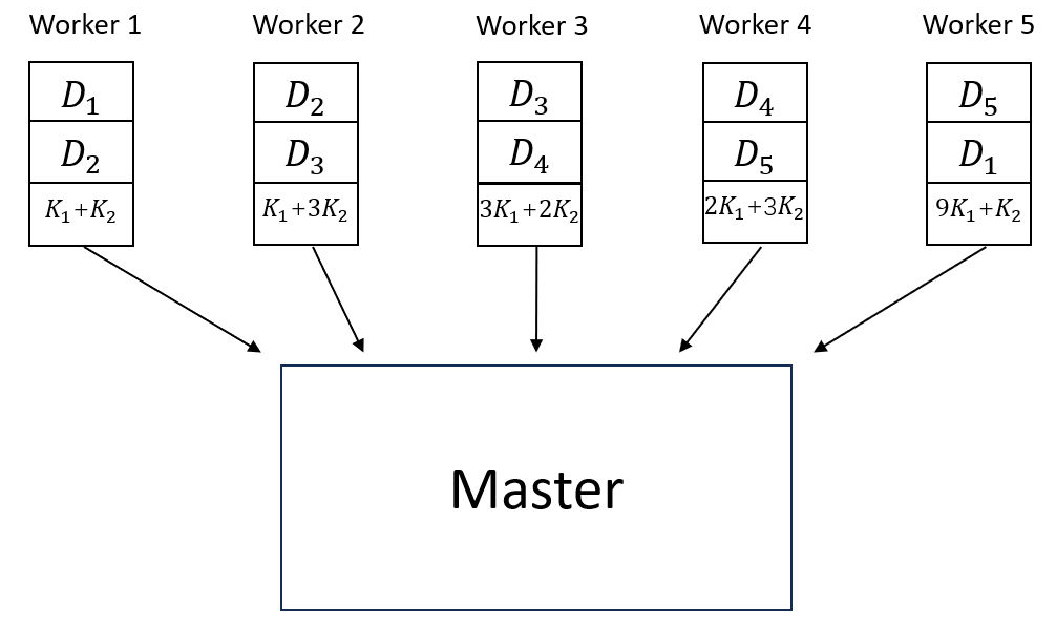
\includegraphics[scale=0.35]{our scheme}}
\caption{\small The individual key size of proposed scheme is 1.}
\label{fig: our scheme}
%\vspace{-5mm}
\end{figure}

We then attempt the computation scheme proposed in \cite{wan2022secure}, which we refer to as the baseline scheme.
 In the baseline scheme, when the demand matrix changes, the key combinations each worker needs to send also change. We randomly assign values to the virtual demands in the matrix \( {\bf F}_2 \), as shown below:

\begin{equation}
{\bf F}_2 = \left[
\begin{array}{ccccccc}
\tikzmark{left1}1 & 1 & 1 & 1 & 1 & \tikzmark{left2} 0 & 0  \\
1 & 2 & 3 & 4 & 5 & 0 & 0 \\
4 & 1 & 1 & 4 & 8 & 1 & 0 \\
3 & 7 & 8 & 7 & 9  \tikzmark{right1}& 0 & 1 \tikzmark{right2} \\
\end{array}
\right].
\label{eq:old F key size}
\end{equation}

\DrawBox[thick, black, dashed]{left1}{right1}{\textcolor{black}{\footnotesize${\bf F}_l$}}
\DrawBox[thick, red, dashed]{left2}{right2}{\textcolor{red}{\footnotesize${\bf F}_r$}}

For each \( n \in [\Nsf] \), we extract the columns corresponding to the data set that worker \(n\) cannot compute in \( {\bf F}_l \), forming a new matrix. By calculating the left null vector of this matrix, we can obtain \( \sv^{n} \). This gives us the matrix \( {\bf S}_2 \), as shown in \eqref{eq:old S key size}:

\begin{equation}
{\bf S}_2 = \left[ \begin{array}{c}
\sv^{1} \\
\sv^{2} \\
\sv^{3} \\
\sv^{4} \\
\sv^{5}
\end{array} \right]
= \begin{bmatrix}
\tikzmark{left4} -35 & 10 & \tikzmark{left5} -3 & 1 \\
-6 & -8  & -1  & 6 \\
-27 & -17  & 5  & 8 \\
-6 & -1  & 1 & 1 \\
-17 & -3 \tikzmark{right4}& 2 & 3 \tikzmark{right5} 
\end{bmatrix}. 
\label{eq:old S key size}
\end{equation}

\DrawBox[thick, black, dashed]{left4}{right4}{\textcolor{black}{\footnotesize${\bf S}_l$}}
\DrawBox[thick, red, dashed]{left5}{right5}{\textcolor{red}{\footnotesize${\bf S}_r$}}

It can be seen that the individual key set stored by the workers is \( \{-3K_1 + K_2, -K_1 + 6K_2, 5K_1 + 8K_2, K_1 + K_2, 2K_1 + 3K_2\} \).

When the demand matrix changes, for example, it becomes
\begin{equation}
{\bf F}' = \begin{bmatrix}
1 & 1 & 1 & 1 & 1 \\
1 & 4 & 9 & 2 & 1 
\end{bmatrix},
\end{equation}
following the same computation scheme as above, we obtain
\begin{equation}
{\bf F}_3 = \left[
\begin{array}{ccccccc}
\tikzmark{left1} 1 & 1 & 1 & 1 & 1 & \tikzmark{left2} 0 & 0  \\
1 & 4 & 9 & 2 & 1 & 0 & 0 \\
8 & 10 & 8 & 3 & 10 & 1 & 0 \\
5 & 9 & 7 & 2 & 8 \tikzmark{right1} & 0 & 1 \tikzmark{right2} \\
\end{array}
\right].
\label{eq:new F key size}
\end{equation}

\DrawBox[thick, black, dashed]{left1}{right1}{\textcolor{black}{\footnotesize${\bf F}_l$}}
\DrawBox[thick, red, dashed]{left2}{right2}{\textcolor{red}{\footnotesize${\bf F}_r$}}

Next, we compute the matrix \( {\bf S}_3 \), which is given by:
\begin{equation}
{\bf S}_3 = \left[ \begin{array}{c}
\sv^{1} \\
\sv^{2} \\
\sv^{3} \\
\sv^{4} \\
\sv^{5}
\end{array} \right]
= \begin{bmatrix}
\tikzmark{left4} 43 & -5 & \tikzmark{left5} -47 & 54 \\
23 & -9  & -3  & 2 \\
44 & -2  & -9  & 6 \\
66 & -2  & -13 & 8 \\
1 & \textcolor{white}{0}0 \tikzmark{right4} & -1 & 1 \tikzmark{right5} 
\end{bmatrix}.
\label{eq:new S key size}
\end{equation}

\DrawBox[thick, black, dashed]{left4}{right4}{\textcolor{black}{\footnotesize${\bf S}_l$}}
\DrawBox[thick, red, dashed]{left5}{right5}{\textcolor{red}{\footnotesize${\bf S}_r$}}

As we can see, when the demand matrix changes, \( {\bf S}_r \) also changes. Consequently, the product of \( {\bf S}_r \) and the identity matrix in \( {\bf F}_r \) also changes. In other words, the workers need to send new key linear combinations, and the key storage requirement for each worker increases. It can be seen that the additional individual key set stored by the workers is \( \{-47K_1 + 54K_2, -3K_1 + 2K_2, -9K_1 + 6K_2, -13K_1 + 8K_2, -K_1 + K_2\} \) i.e., each worker needs to store the complete keys \( K_1 \) and \( K_2 \) to handle the different demand matrices, meaning the individual key size is 2, as shown in Fig.~\ref{fig: other scheme}.

\begin{figure}%[ht]
%\vspace{-2mm}
\centerline{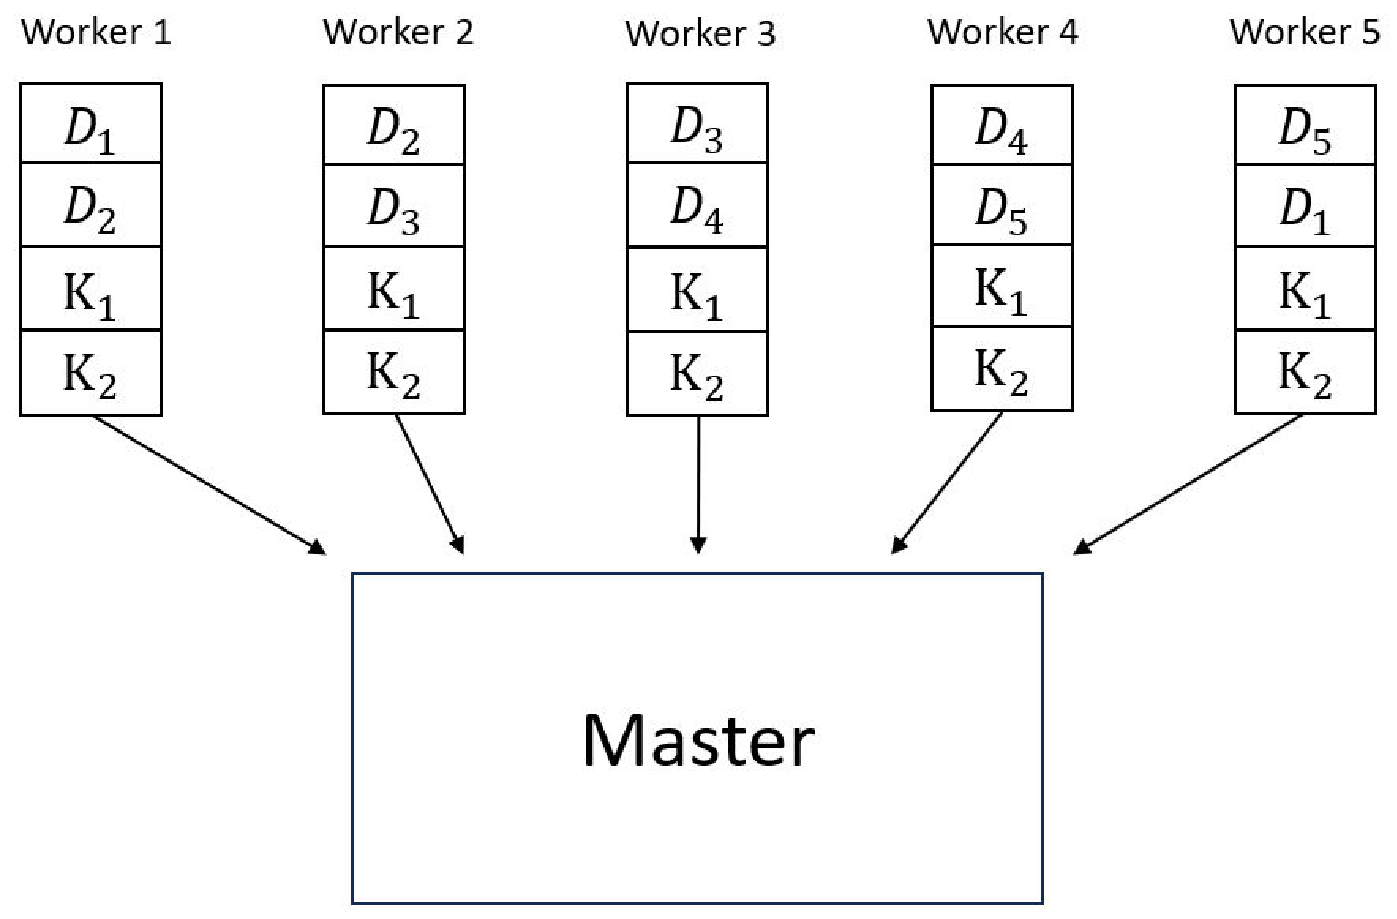
\includegraphics[scale=0.25]{other scheme}}
\caption{\small The individual key size of the baseline scheme is 2.}
\label{fig: other scheme}
%\vspace{-5mm}
\end{figure}



Notice that in our scheme, when we change the demand matrix, the number of unknowns and resulting equations remain the same, implying that we can still solve for a new set of unknowns. By keeping ${\bf S}_r$ and ${\bf F}_r$ fixed, the key combinations sent by each worker remain constant. The individual key set stored by workers is still $\{K_1 +K_2, K_1 +3K_2, 3K_1 +2K_2, 2K_1 +3K_2, 9K_1 +K_2\}$. In other words, the individual key size is 
\begin{align}
    \Qsf_{\rm s} = \frac{\Ksf_{\rm c}}{\msf + \Ksf_{\rm c} - 1} = \frac{\Rsf^{\star}}{\Nsf_{\rm r}} = 1,
\end{align}
satisfying~\eqref{eq:Qs}.
\end{example}

\begin{figure}%[ht]
%\vspace{-2mm}
\centerline{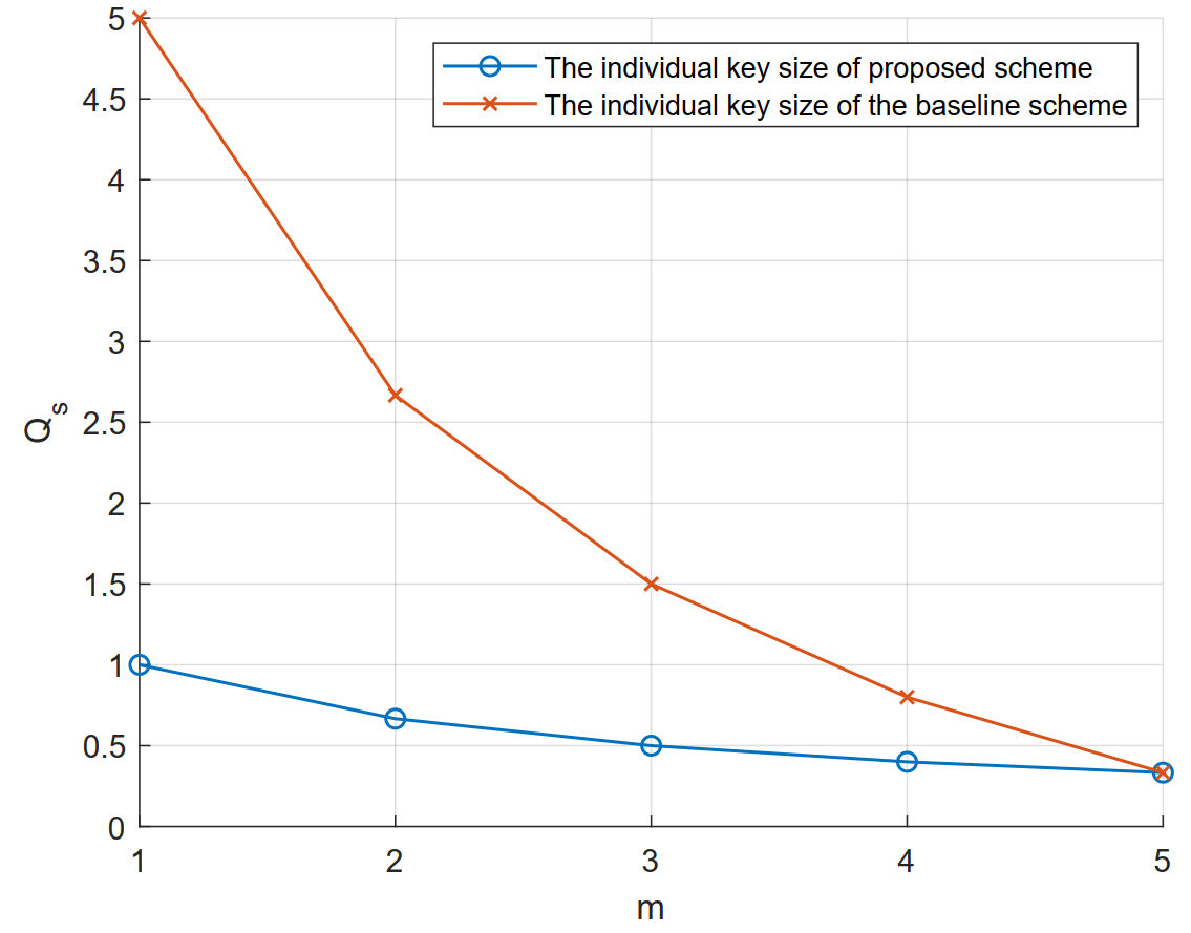
\includegraphics[scale=0.33]{compare}}
\caption{\small Numerical evaluations for the individual key size of the $(\Ksf, \Nsf, \Nsf_{\rm r}, \Ksf_{\rm c}, \msf) = (11, 11, 7, 2, \msf)$ secure distributed linearly separable computation problem.}
\label{fig: compare}
%\vspace{-5mm}
\end{figure}

In Fig.~\ref{fig: compare}, we consider the secure distributed linearly separable computation problem where $\Nsf = \Ksf = 11$, $\Nsf_{\rm r} = 7$, and $\Ksf_{\rm c}=2$.
It can be seen that our scheme significantly outperforms the baseline scheme in terms of individual key size.


We now generalize the distributed computing scheme described in Example~\ref{ex:individual key size example}. The general case considers $\Ksf_{\rm c}= \frac{\Ksf}{\Nsf} \usf$, where $\usf \in [\Nsf_{\rm r}-\msf+1]$ and $\usf (\Nsf_{\rm r}-\msf-\usf+1) + \frac{\msf+\usf-1}{\usf}$. 
During the data assignment phase, we adopt the cyclic assignment strategy, where each worker is assigned $\Msf = \frac{\Ksf}{\Nsf} (\Nsf - \Nsf_{\rm r} + \msf)$ datasets.

\paragraph*{Computing phase}
To achieve the optimal communication cost \( R^* = \Nsf_{\rm r} \frac{\Ksf_{\rm c}}{\msf + \usf - 1} \), we first divide each message \( W_k, k \in [\Ksf] \), into \( \msf + \usf - 1 \) non-overlapping and equal-length sub-messages, denoted as \( W_{k} = \{W_{k,j} : j \in [\msf + \Ksf_{\rm c} - 1]\} \), so that each sub-message contains \( \frac{\Lsf}{\msf + \usf - 1} \) symbols in \( \mathbb{F}_{\qsf} \). Additionally, to satisfy the security constraint in \eqref{eq:security}, we generate \(\Qsf =  \Nsf_{\rm r}\Ksf_{\rm c} - \Ksf_{\rm c} ( \msf + \usf - 1) \) independent keys, each of size \( \frac{\Lsf}{\msf + \usf - 1} \). Each worker is tasked to send \( \Ksf_{\rm c}\) linear combinations of sub-messages. 
From the answers of \( \Nsf_{\rm r}  \) workers, the master receives a total of \( \Nsf_{\rm r} \Ksf_{\rm c} \) linear combinations of sub-messages, which contain the desired \( (\msf + \usf - 1) \Ksf_{\rm c}  \) linear combinations. Consequently, 
we generate 
$$
\vsf = \Nsf_{\rm r} \Ksf_{\rm c} - (\msf+\usf-1)\Ksf_{\rm c} =\Ksf_{\rm c} (\Nsf_{\rm r}-\msf-\usf+1)
$$
 virtually requested linear combinations; Thus, the effective demand matrix ${\bf F}$ has dimension $\Nsf_{\rm r}\Ksf_{\rm c} \times \Ksf(\msf+\usf-1)$, with its form shown at the top of the next page in~\eqref{eq:general F}, where ${\bf F}_{\msf+\usf}$ corresponds to the key portion.
 For convenience, we set the part of the virtual demand corresponding to the keys as an identity matrix.
 
    \begin{figure*}
\begin{equation}
{\bf F} =\left[
\begin{array}{ccccccccccccc}     
\tikzmark{left1} \textcolor{white}{0} f_{1,1} &\cdots &  \textcolor{white}{0} f_{1,\Ksf}& \tikzmark{left2} \textcolor{white}{000} 0&\cdots  & \textcolor{white}{000} 0& \cdots & \tikzmark{left3}  \textcolor{white}{00000} 0 \textcolor{white}{00000} & \cdots &  \textcolor{white}{00000} 0 \textcolor{white}{00000} & \tikzmark{left4}0&\cdots  &0\\
\vdots &\ddots & \vdots &  \vdots & \ddots  & \vdots & \ddots & \vdots  & \ddots & \vdots& \vdots  & \ddots & \vdots\\
 f_{\Ksf_{\rm c},1} &\cdots & f_{\Ksf_{\rm c},\Ksf}&  \textcolor{white}{00} 0&\cdots  & \textcolor{white}{00} 0& \cdots &   \textcolor{white}{00000} 0 \textcolor{white}{00000} & \cdots & \textcolor{white}{00000} 0 \textcolor{white}{00000}&0&\cdots  &0\\
\textcolor{white}{00}0  &\cdots &\textcolor{white}{00}0  &  f_{1,1} &\cdots  & f_{1,\Ksf} & \cdots &   \textcolor{white}{00000} 0 \textcolor{white}{00000}& \cdots & \textcolor{white}{00000} 0 \textcolor{white}{00000}&0&\cdots  &0 \\
\vdots &\ddots & \vdots &  \vdots & \ddots  & \vdots & \ddots & \vdots  & \ddots & \vdots& \vdots  & \ddots & \vdots\\
\textcolor{white}{00}0  &\cdots &\textcolor{white}{00}0  &  f_{\Ksf_{\rm c},1} &\cdots  & f_{\Ksf_{\rm c},\Ksf} & \cdots &   \textcolor{white}{00000} 0 \textcolor{white}{00000} & \cdots &\textcolor{white}{00000} 0 \textcolor{white}{00000}&0&\cdots  &0\\
\vdots &\ddots & \vdots &  \vdots & \ddots  & \vdots & \ddots & \vdots  & \ddots & \vdots& \vdots  & \ddots & \vdots\\
 \textcolor{white}{00}0  &\cdots &\textcolor{white}{00}0  &  \textcolor{white}{00}0 &\cdots  & \textcolor{white}{00}0 & \cdots &  f_{1,1}  & \cdots &  f_{1,\Ksf}&0&\cdots  &0 \\
\vdots &\ddots & \vdots &  \vdots & \ddots  & \vdots & \ddots & \vdots  & \ddots & \vdots& \vdots  & \ddots & \vdots\\
 \textcolor{white}{00}0  &\cdots &\textcolor{white}{00}0  &  \textcolor{white}{00}0 &\cdots  & \textcolor{white}{00}0 & \cdots &  f_{\Ksf_{\rm c},1}  & \cdots &  f_{\Ksf_{\rm c},\Ksf}&0&\cdots  &0 \\
  a_{1,1}&\cdots  &   a_{1,\Ksf} & a_{1,\Ksf+1} &\cdots & a_{1,2\Ksf}& \cdots &  a_{1,(\msf+\usf-2)\Ksf+1 } &\cdots  & a_{1, (\msf+\usf-1)\Ksf} &1&\cdots  &0\\
\vdots &\ddots & \vdots &  \vdots & \ddots  & \vdots & \ddots & \vdots  & \ddots & \vdots& \vdots  & \ddots & \vdots\\
    a_{\vsf,1}&\cdots  &   a_{\vsf,\Ksf} \tikzmark{right1}  & a_{\vsf ,\Ksf+1} &\cdots & a_{\vsf,2\Ksf} \tikzmark{right2}  & \cdots &  a_{\vsf,(\msf+\usf-2)\Ksf+1 } &\cdots  & a_{\vsf, (\msf+\usf-1)\Ksf} \tikzmark{right3} &0&\cdots  &\textcolor{white}{0}1\tikzmark{right4} \ \ 
\end{array}
\right]. \label{eq:general F}
\end{equation}
\DrawBox[thick, black, dashed]{left1}{right1}{\textcolor{black}{\footnotesize${\bf F}_1$}}
\DrawBox[thick, red, dashed]{left2}{right2}{\textcolor{red}{\footnotesize${\bf F}_2$}}
\DrawBox[thick, blue, dashed]{left3}{right3}{\textcolor{blue}{\footnotesize${\bf F}_{\msf+\usf-1}$}}
\DrawBox[thick, blue, dashed]{left4}{right4}{\textcolor{orange}{\footnotesize${\bf F}_{\msf+\usf}$}}
   \end{figure*}

Our coding strategy is to let each worker \( n \in [\Nsf] \) send \( \Ksf_{\rm c} \) linear combinations of sub-messages
\begin{align}
\sv^{n,i} {\bf F} [W_{1,1}; \ldots; W_{\Ksf,1}; W_{1,2}; \ldots; W_{\Ksf,\msf + \usf - 1}], \label{eq:general transmitted linear combinations}
\end{align}
where \( i \in [\Ksf_{\rm c}] \), for a total of \( \frac{\Ksf_{\rm c} \Lsf}{\msf + \usf - 1} \) symbols, coinciding with the converse bound. Note that $\sv^{n,i} $ is vector with length $\Nsf_{\rm r}\Ksf_{\rm c} $. The overall coding matrix ${\bf S}$ is further expanded, as shown at the top of the next page.

    \begin{figure*}
\begin{equation}
 {\bf S}=  \left[ \begin{array}{c}
\sv^{1,1}\\
\vdots\\
\sv^{1,\Ksf_{\rm c}}\\
\sv^{2,1}\\
\vdots\\
\sv^{\Nsf,\Ksf_{\rm c}}
\end{array} \right] =  
\begin{bmatrix} \ 
\tikzmark{left4} \textcolor{white}{0} s^{1,1}_1 & \cdots& s^{1,1}_{\Ksf_{\rm c}} & \cdots & 
\tikzmark{left6} s^{1,1}_{(\msf+\usf-2)\Ksf_{\rm c}+1} &\cdots & s^{1,1}_{(\msf+\usf-1)\Ksf_{\rm c}}  &   
  \tikzmark{left7} \textcolor{white}{0} b^{1,1}_{1}  & \cdots&  b^{1,1}_{\vsf}   \\
\vdots & \ddots &  \vdots  & \ddots & \vdots & \ddots & \vdots & \vdots & \ddots &\vdots \\
  s^{1,\Ksf_{\rm c}}_1 & \cdots& s^{1,\Ksf_{\rm c}}_{\Ksf_{\rm c}} &   \cdots & 
 s^{1,\Ksf_{\rm c}}_{(\msf+\usf-2)\Ksf_{\rm c}+1} &\cdots & s^{1,\Ksf_{\rm c}}_{(\msf+\usf-1)\Ksf_{\rm c}}  &   
 b^{1,\Ksf_{\rm c}}_{1}  & \cdots& b^{1,\Ksf_{\rm c}}_{\vsf}   \\
   s^{2,1}_1 & \cdots& s^{2,1}_{\Ksf_{\rm c}} &   \cdots & 
 s^{2,1}_{(\msf+\usf-2)\Ksf_{\rm c}+1} &\cdots & s^{2,1}_{(\msf+\usf-1)\Ksf_{\rm c}}  &   
b^{2,1}_{1}  & \cdots&  b^{2,1}_{\vsf}   \\
\vdots & \ddots &  \vdots  & \ddots & \vdots & \ddots & \vdots & \vdots & \ddots &\vdots \\
 s^{\Nsf,\Ksf_{\rm c}}_1 & \cdots& s^{\Nsf,\Ksf_{\rm c}}_{\Ksf_{\rm c}} \tikzmark{right4} &      \cdots & 
 s^{\Nsf,\Ksf_{\rm c}}_{(\msf+\usf-2)\Ksf_{\rm c}+1} &\cdots & s^{\Nsf,\Ksf_{\rm c}}_{(\msf+\usf-1)\Ksf_{\rm c}} \tikzmark{right6}  &   
 b^{\Nsf,\Ksf_{\rm c}}_{1}  & \cdots&  b^{\Nsf,\Ksf_{\rm c}}_{\vsf} \tikzmark{right7}  \ \
 \end{bmatrix}. \label{eq:division of S}
\end{equation}
 \DrawBox[thick, black,  dashed ]{left4}{right4}{\textcolor{black}{\footnotesize${\bf S}_1$}}
\DrawBox[thick, blue, dashed]{left6}{right6}{\textcolor{blue}{\footnotesize${\bf S}_{\msf+\usf-1}$}}
\DrawBox[thick, red, dashed]{left7}{right7}{\textcolor{red}{\footnotesize${\bf S}_{\msf+\usf}$}}

\rule{\textwidth}{0.2pt} % 创建分割线
   \end{figure*}

For each \( n \in [\Nsf] \), worker \( n \) cannot compute the \( \text{Mod}(n+l,\Ksf) \) datasets, where \( l \in [\Msf:\Ksf - 1] \). This constraint can be expressed as:
\begin{align}
\sv^{n,i} \cv_{\text{Mod}(n+l,\Ksf) + (j-1)\Ksf} W_{\text{Mod}(n+l,\Ksf), j} = 0,  \label{eq: transmit constraint}
\end{align}
where \( i \in [\Ksf_{\rm c}] \) denotes the \( i^{\text{th}} \) linear combination sent by worker \( n \), and \( \cv_{k} \) is the \( k^{\text{th}} \) column of matrix \( {\bf F} \).

Additionally, for any subset \(\Ac \subseteq [\Nsf]\) with \( |\Ac| = \Nsf_{\rm r} \), the master must recover the desired linear combinations from the responses of workers in \(\Ac\). This requires:
\begin{align}
\begin{aligned}
&[\sv^{\Ac(1),1}; \ldots; \sv^{\Ac(1),\Ksf_{\rm c}}; \sv^{\Ac(2),1}; \ldots; \sv^{\Ac(\Nsf_{\rm r}),\Ksf_{\rm c}}] \ \text{to be full rank}, \\
&\forall \Ac \subseteq [\Nsf]: |\Ac| = \Nsf_{\rm r}.
\end{aligned} \label{eq:decodability constraint}
\end{align}

Our goal is to determine the variables in \({\bf S}\) (i.e., \( s^{n,j}_{i} \) where \( n \in [\Nsf], j \in [\Ksf_{\rm c}], i \in [(\msf+\usf-1)\Ksf_{\rm c}] \), and \( b^{n,j}_{i} \) where \( n \in [\Nsf], j \in [\Ksf_{\rm c}], i \in [\vsf] \)), and in \({\bf F}\) (i.e., \( a_{i,k} \) where \( i \in [\vsf], k \in [(\msf+\usf-1)\Ksf] \)), such that the constraints in~\eqref{eq: transmit constraint} and~\eqref{eq:decodability constraint} are satisfied.


We divide the matrix ${\bf F}$ into $\msf+\usf-1$ sub-matrices, ${\bf F}_1, \ldots, {\bf F}_{\msf+\usf-1}$, each with dimensions $\Nsf_{\rm r}\Ksf_{\rm c} \times \Ksf$, as shown in~\eqref{eq:general F}. Similarly, matrix ${\bf S}$ is divided into $\msf+\usf$ sub-matrices: ${\bf S}_1, \ldots, {\bf S}_{\msf+\usf-1}$, each with dimensions $\Nsf \Ksf_{\rm c} \times \Ksf_{\rm c}$, and ${\bf S}_{\msf+\usf}$ with dimensions $\Nsf \Ksf_{\rm c} \times \vsf$, as illustrated in~\eqref{eq:division of S}.

As in Example~\ref{ex:individual key size example}, the proposed computing scheme consists of three main steps:
\begin{enumerate}
\item Choose values for the variables in ${\bf S}_{\msf+\usf}$, which are associated with the coefficients of the key linear combinations sent by the workers.
\item Use the constraints in~\eqref{eq: transmit constraint}, which become linear after fixing ${\bf S}_{\msf+\usf}$, to solve for the remaining variables;
\item Verify that the constraints in~\eqref{eq:decodability constraint} are satisfied, ensuring the scheme is decodable.
\end{enumerate}


 

\paragraph*{Step 1}
We assign values to ${\bf S}_{\msf+\usf}$ in the following form:
\begin{align}
{\bf S}_{\msf+\usf}&= \left[ \begin{array}{ccccccc}
 b^{1,1}_{1}  & \cdots &  b^{1,1}_{\frac{\vsf}{\Ksf_{\rm c}}}  &\cdots & b^{1,1}_{\frac{(\Ksf_{\rm c}-1)\vsf}{\Ksf_{\rm c}}+1}& \cdots& b^{1,1}_{\vsf} \\ 
  b^{1,2}_{1}  & \cdots &  b^{1,2}_{\frac{\vsf}{\Ksf_{\rm c}}}  &\cdots & b^{1,2}_{\frac{(\Ksf_{\rm c}-1)\vsf}{\Ksf_{\rm c}}+1}& \cdots& b^{1,2}_{\vsf} \\ 
 \vdots &   \ddots&  \vdots&   \ddots& \vdots &\ddots &\vdots\\
 b^{1,\Ksf_{\rm c}}_{1} &\cdots &  b^{1,\Ksf_{\rm c}}_{\frac{\vsf}{\Ksf_{\rm c}}}  & \cdots  & b^{1,\Ksf_{\rm c}}_{\frac{(\Ksf_{\rm c}-1)\vsf}{\Ksf_{\rm c}}+1}& \cdots & b^{1,\Ksf_{\rm c}}_{\vsf} \\ 
 b^{2,1}_{1}   &\cdots &  b^{2,1}_{\frac{\vsf}{\Ksf_{\rm c}}}  & \cdots &  b^{2,1}_{\frac{(\Ksf_{\rm c}-1)\vsf}{\Ksf_{\rm c}}+1}& \cdots & b^{2,1}_{\vsf} \\  
 \vdots &   \ddots&  \vdots&   \ddots& \vdots &\ddots &\vdots\\
b^{\Nsf,\Ksf_{\rm c}}_{1}  &\cdots &  b^{\Nsf,\Ksf_{\rm c}}_{\frac{\vsf}{\Ksf_{\rm c}}}  & \cdots & b^{\Nsf,\Ksf_{\rm c}}_{\frac{(\Ksf_{\rm c}-1)\vsf}{\Ksf_{\rm c}}+1}& \cdots & b^{\Nsf,\Ksf_{\rm c}}_{\vsf}   
\end{array} \right]  \nonumber \\
&= 
\left[ \begin{array}{cccccccccccc}
* & \cdots & * & 0 &\cdots & 0  &0 & \cdots& 0& 0& \cdots& 0\\ 
0 & \cdots & 0 & * &\cdots & * &0  & \cdots& 0& 0& \cdots& 0\\ 
 \vdots &   \ddots&  \vdots&  \vdots&  \ddots&  \vdots& \vdots& \ddots&  \vdots& \vdots &\ddots &\vdots\\
0 &\cdots &  0 &0 &\cdots &0  & 0& \cdots & 0 &*& \cdots & * \\ 
*   &\cdots &  *  &0 &\cdots & 0  &0& \cdots& 0&  0& \cdots &0 \\  
 \vdots &   \ddots&  \vdots&  \vdots&  \ddots&  \vdots& \vdots& \ddots&  \vdots& \vdots &\ddots &\vdots\\
     0  &\cdots & 0 & 0 &\cdots & 0 &0 & \cdots &0 & * & \cdots & *
\end{array} \right]
,\label{eq:S_{m+u}}
\end{align}
where each `$*$' represents a uniformly i.i.d. symbol in $\mathbb{F}_{\qsf}$. 

This structure ensures that the constraints in~\eqref{eq: transmit constraint} are linearly independent with respect to the remaining variables, which will be determined in the next step.



\paragraph*{Step 2}
We now determine the variables in matrices \( {\bf F} \) and \( {\bf S} \). Fixing one \( i \in [\Ksf_{\rm c}] \) and one \( j \in [\msf+\usf-1] \), the constraints in~\eqref{eq: transmit constraint} become:
\begin{align}
\begin{aligned}
0 &= \sum_{i_1 \in [\Ksf_{\rm c}]} f_{i_1,\text{Mod}(n+l,\Ksf)} \ s^{n,i}_{(j-1)\Ksf_{\rm c}+i_1} \\
&\quad + \sum_{i_2 \in [\vsf]} b^{n,i}_{i_2} \ a_{i_2,(j-1)\Ksf+\text{Mod}(n+l,\Ksf)}.
\end{aligned}
\label{eq:constraints}
\end{align}

In~\eqref{eq:constraints}, the coefficients \( f_{i_1,k} \) are elements of the demand matrix \({\bf F}\), and the values \( b^{n,i}_{i_2} \) were determined in Step 1. The total number of variables in~\eqref{eq:constraints} is:
\begin{align}
\Nsf \Ksf_{\rm c} + \frac{\vsf}{\Ksf_{\rm c}} \Ksf 
&= \Nsf \frac{\Ksf}{\Nsf} \usf + (\Nsf_{\rm r} - \msf - \usf + 1) \Ksf \notag \\
&= \Ksf (\Nsf_{\rm r} - \msf + 1). \label{eq:variables}
\end{align}

There are a total of \( \Ksf(\Nsf_{\rm r}-\msf) \) constraints in~\eqref{eq:constraints}. Since the number of variables exceeds the number of constraints, we solve the resulting system of equations, which is likely to have a solution. For each \( n \in [\Nsf] \), we can assign:
\begin{align}
s^{n,i}_{(j-1)\Ksf_{\rm c}+(p-1)\usf +\text{Mod}(n,\usf)}, \quad \forall p \in \left[\Ksf/\Nsf\right], \label{eq:choose value}
\end{align}
random values uniformly i.i.d. over \( \mathbb{F}_{\qsf} \). This determines \( \Ksf \) variables out of the \( \Ksf(\Nsf_{\rm r}-\msf + 1) \), leaving \( \Ksf(\Nsf_{\rm r}-\msf) \) variables to be solved by \( \Ksf(\Nsf_{\rm r}-\msf) \) linear equations.
As shown in Appendix~\ref{sec:feasibility proof}, these equations are linearly independent with high probability, allowing us to solve for all variables in~\eqref{eq:variables}.

By iterating over all pairs \((i,j)\) where \( i \in [\Ksf_{\rm c}] \) and \( j \in [\msf+\usf-1] \), we determine all elements in \({\bf S}\) and \({\bf F}\).



\paragraph*{Step 3}
As shown in Appendix~\ref{sec:feasibility proof}, the constraints in~\eqref{eq:decodability constraint} hold with high probability. Consequently, each worker \( n \in [\Nsf] \) computes and transmits \(\Ksf_{\rm c}\) linear combinations of sub-messages:
\begin{align}
\begin{aligned}
&\sv^{n,i} {\bf F} [W_{1,1}; \ldots; W_{\Ksf,1}; W_{1,2}; \ldots; W_{\Ksf,\msf+\isf-1}] \\
&= \sv^{n,i}[{F_1}; \ldots; {F_{\Ksf_{\rm c}}}],
\end{aligned}
\end{align}
where \( i \in [\Ksf_{\rm c}] \).

\paragraph*{Decoding Phase}
Let $\Ac \subseteq [\Nsf]$ be the set of responding workers with $ |\Ac| = \Nsf_{\rm r} $. The master receives a total of $\Nsf_{\rm r}\Ksf_{\rm c}$ messages:
\begin{align}
{\bf X}_{\Ac} =
&[\sv^{\Ac(1),1}; \ldots; \sv^{\Ac(1),\Ksf_{\rm c}}; \sv^{\Ac(2),1}; \ldots; \sv^{\Ac(\Nsf_{\rm r}),\Ksf_{\rm c}}]  \nonumber \\
& \text{ × } [{F_1}; \ldots; {F_{\Ksf_{\rm c}}}].
\end{align}

Since the matrix \([\sv^{\Ac(1),1}; \ldots; \sv^{\Ac(\Nsf_{\rm r}),\Ksf_{\rm c}}]\) is full-rank, the master computes:
\begin{align}
[\sv^{\Ac(1),1}; \ldots; \sv^{\Ac(\Nsf_{\rm r}),\Ksf_{\rm c}}]^{-1} {\bf X}_{\Ac},
\end{align}
recovering \([{F_1}; \ldots; {F_{\Ksf_{\rm c}}}]\), which contains the required linear combinations.
It is worth noting that the above process remains unchanged regardless of the demand. Thus, each worker can consistently send the invariant linear combinations of keys, as the coefficients of the key linear combinations have already been fixed in Step 1. This implies that each worker only needs to store \(\Ksf_{\rm c}\) key combinations, with a total size of
\begin{align}
    \Qsf_{\rm s} = \frac{\Ksf_{\rm c}}{\msf + \usf - 1} = \frac{\Rsf^{\star}}{\Nsf_{\rm r}}
\end{align}
satisfying~\eqref{eq:Qs}.

\section{Conclusion}
We focus on the secure distributed linearly separable computation problem, which prevents the master from accessing any information about the dataset besides the task function. We first research the minimum key size under general computation cost while achieving optimal communication cost. For this purpose, we propose a new computing scheme with a novel assignment strategy. The computing scheme can cover the optimality results of the computational scheme with fractional repetition assignment. The new computing scheme is also applicable to the case of minimal computational cost in \cite{wan2022secure}.
Then we propose a computing scheme that achieves the minimum individual key size under the optimal communication cost when the demand is unknown.




\iffalse
We first attempt the computation scheme proposed in ~\cite{m=1}. We begin by randomly assigning values to the virtual demands in the matrix \( {\bf F} \), as shown below:

\begin{equation}
{\bf F} = \left[
\begin{array}{ccccccc}
\tikzmark{left1}1 & 1 & 1 & 1 & 1 & \tikzmark{left2} 0 & 0  \\
1 & 2 & 3 & 4 & 5 & 0 & 0 \\
4 & 1 & 1 & 4 & 8 & 1 & 0 \\
3 & 7 & 8 & 7 & 9  \tikzmark{right1}& 0 & 1 \tikzmark{right2} \\
\end{array}
\right].
\label{eq:old F key size}
\end{equation}

\DrawBox[thick, black, dashed]{left1}{right1}{\textcolor{black}{\footnotesize${\bf F}_1$}}
\DrawBox[thick, red, dashed]{left2}{right2}{\textcolor{red}{\footnotesize${\bf F}_2$}}

For each \( n \in [\Nsf] \), we extract the columns corresponding to the data set that worker \(n\) cannot compute in \( {\bf F}_1 \), forming a new matrix. By calculating the left null vector of this matrix, we can obtain \( \sv^{n} \). This gives us the matrix \( {\bf S} \), as shown in \eqref{eq:old S key size}:

\begin{equation}
{\bf S} = \left[ \begin{array}{c}
\sv^{1} \\
\sv^{2} \\
\sv^{3} \\
\sv^{4} \\
\sv^{5}
\end{array} \right]
= \begin{bmatrix}
\tikzmark{left4} -35 & 10 & \tikzmark{left5} -3 & 1 \\
-6 & -8  & -1  & 6 \\
-27 & -17  & 5  & 8 \\
-6 & -1  & 1 & 1 \\
-17 & -3 \tikzmark{right4}& 2 & 3 \tikzmark{right5} 
\end{bmatrix}. 
\label{eq:old S key size}
\end{equation}

\DrawBox[thick, black, dashed]{left4}{right4}{\textcolor{black}{\footnotesize${\bf S}_1$}}
\DrawBox[thick, red, dashed]{left5}{right5}{\textcolor{red}{\footnotesize${\bf S}_2$}}

When the demand matrix \( {\bf F}' \) changes, for example, it becomes
\begin{equation}
{\bf F}' = \begin{bmatrix}
1 & 1 & 1 & 1 & 1 \\
1 & 4 & 9 & 2 & 1 
\end{bmatrix},
\end{equation}
following the same computation scheme as above, we obtain
\begin{equation}
{\bf F} = \left[
\begin{array}{ccccccc}
\tikzmark{left1} 1 & 1 & 1 & 1 & 1 & \tikzmark{left2} 0 & 0  \\
1 & 4 & 9 & 2 & 1 & 0 & 0 \\
8 & 10 & 8 & 3 & 10 & 1 & 0 \\
5 & 9 & 7 & 2 & 8 \tikzmark{right1} & 0 & 1 \tikzmark{right2} \\
\end{array}
\right].
\label{eq:new F key size}
\end{equation}

\DrawBox[thick, black, dashed]{left1}{right1}{\textcolor{black}{\footnotesize${\bf F}_1$}}
\DrawBox[thick, red, dashed]{left2}{right2}{\textcolor{red}{\footnotesize${\bf F}_2$}}

Next, we compute the matrix \( {\bf S} \), which is given by:
\begin{equation}
{\bf S} = \left[ \begin{array}{c}
\sv^{1} \\
\sv^{2} \\
\sv^{3} \\
\sv^{4} \\
\sv^{5}
\end{array} \right]
= \begin{bmatrix}
\tikzmark{left4} 43 & -5 & \tikzmark{left5} -47 & 54 \\
23 & -9  & -3  & 2 \\
44 & -2  & -9  & 6 \\
66 & -2  & -13 & 8 \\
1 & \textcolor{white}{0}0 \tikzmark{right4} & -1 & 1 \tikzmark{right5} 
\end{bmatrix}.
\label{eq:new S key size}
\end{equation}

\DrawBox[thick, black, dashed]{left4}{right4}{\textcolor{black}{\footnotesize${\bf S}_1$}}
\DrawBox[thick, red, dashed]{left5}{right5}{\textcolor{red}{\footnotesize${\bf S}_2$}}

As we can see, when the demand matrix \( {\bf F}' \) changes, \( {\bf S}_2 \) also changes. Consequently, the product of \( {\bf S}_2 \) and the identity matrix in \( {\bf F}_2 \) also changes. This means that the workers need to send new key linear combinations, and the key storage requirement for each worker increases. Under this computation scheme, each worker needs to store the complete keys \( K_1 \) and \( K_2 \) to handle the different demand matrices, meaning the individual key size is 2.

In the following, we will introduce our proposed scheme and compare it with the previous schemes in terms of individual key size.

\fi









  \appendices


\section{Proof of Theorem~\ref{thm:bound of η}}
\label{sec:bound proof}
By the security constraint in~\eqref{eq:security}, the master can only obtain $W_1+\cdots+W_{\Ksf}$ without accessing any additional information about the messages, even after receiving answers from all workers. Let $X_{\Sc}=\{X_n: n \in \Sc\}$. From~\eqref{eq:security}, we derive:
\begin{subequations}
\begin{align}
0 &= I(W_1, \ldots, W_{\Ksf}; X_{[\Nsf]} | W_1+W_2+\cdots+W_{\Ksf}) \\
  &= H(X_{[\Nsf]} | W_1+W_2+\cdots+W_{\Ksf}) - H(X_{[\Nsf]} | W_1, \ldots, W_{\Ksf}) \\
  &\geq H(X_{[\Nsf]} | W_1+W_2+\cdots+W_{\Ksf}) \nonumber\\
  &- H(Q, W_1, \ldots, W_{\Ksf} | W_1, \ldots, W_{\Ksf}) \label{eq:function of QW} \\
  &= H(X_{[\Nsf]} | W_1+W_2+\cdots+W_{\Ksf}) - H(Q) \label{eq:independent noise} \\
  &= H(X_{[\Nsf]}) - I(X_{[\Nsf]}; W_1+W_2+\cdots+W_{\Ksf}) - H(Q) \\
  &\geq H(X_{[\Nsf]}) - H(W_1+W_2+\cdots+W_{\Ksf}) - H(Q), \label{eq:shannon}
\end{align}
\end{subequations}
where~\eqref{eq:function of QW} follows from the fact that $X_{[\Nsf]}$ is a function of $Q$ and $W_1, \ldots, W_{\Ksf}$, and~\eqref{eq:independent noise} relies on $Q$ being independent of $W_1, \ldots, W_{\Ksf}$.

From~\eqref{eq:shannon}, we further obtain:
\begin{subequations}
\begin{align}
\eta \Lsf &\geq H(Q) \geq H(X_{[\Nsf]}) - H(W_1+\cdots+W_{\Ksf}) \\
          &\geq H(X_{[\Nsf]}) - \Lsf \label{eq:W1 inde} \\
          &\geq H(X_{s_1}, \ldots, X_{s_{|\sv|}}) - \Lsf \\
          &\geq  \frac{|\sv|\Lsf}{\msf} - \Lsf, \label{eq:lemma converse all term}
\end{align}
\end{subequations}
where~\eqref{eq:W1 inde} follows from the independence of $\Ksf$ messages, each uniformly i.i.d. over $[\mathbb{F}_{\qsf}]^{\Lsf}$, and~\eqref{eq:lemma converse all term} is derived using the chain rule of entropy.

Note that worker $s_i$ always contains at least one message $W_{s_i}$ which can not be computed by $m$ workers from $\{s_1, \ldots, s_{i-1}\}$. Consider the case that apart from $\Nsf - \Nsf_{\rm r}$ stragglers, there are exactly $m$ workers who can compute $W_{s_i}$. Then,  the entropy of messages from these workers should be larger than $\Lsf$.  



\section{Feasibility Proof   of  the Proposed Computing Scheme in Section~\ref{sec:sche}}
\label{sec:feasibility proof}
First, we consider the $(\Ksf, \Nsf, \Nsf_{\rm r}, \Ksf_{\rm c}, \msf) = (\Nsf, \Nsf, \Nsf_{\rm r}, \usf, \msf)$ distributed linearly separable computation problem, where $\Nsf \geq \usf(\Nsf_{\rm r}-\msf-\usf+1) + \frac{\msf+\usf-1}{\usf} $. We prove that the system of linear equations given in~\eqref{eq:constraints} is solvable with high probability, and the constraints in~\eqref{eq:decodability constraint} are also satisfied with high probability.
Next, we prove that if the proposed scheme works with high probability for $(\Ksf, \Nsf, \Nsf_{\rm r}, \Ksf_{\rm c}, \msf) = (\Nsf, \Nsf, \Nsf_{\rm r}, \usf, \msf)$, then it also works with high probability for $(\Ksf, \Nsf, \Nsf_{\rm r}, \Ksf_{\rm c}, \msf) = (\asf\Nsf, \Nsf, \Nsf_{\rm r}, \asf\usf, \msf)$ distributed linearly separable computation problem, where $\asf = \frac{\Ksf}{\Nsf}$ is a positive integer.
\subsection{\texorpdfstring{$\Nsf = \Ksf$}{Nsf = Ksf}}
   \label{sub:proof K=N}
We use the Schwartz-Zippel Lemma~\cite{lemma1,lemma2,lemma3} to prove the feasibility of the proposed computation scheme. This method has already been applied in~\cite[Appendix C]{m=1} to demonstrate the feasibility of the computation scheme for the case where \(\msf = 1\).

Recall that for each \( i \in [\Ksf_{\rm c}] \) and \( j \in [\msf+\usf-1] \), in Step 2 of the proposed scheme, we obtain \( \Ksf(\Nsf_{\rm r}-\msf) \) linear equations as shown in \eqref{eq:constraints}. After determining the values of the \( \Ksf \) elements in \eqref{eq:choose value}, the system of linear equations still has \( \Ksf(\Nsf_{\rm r}-\msf) \) unknowns to be determined(the vector representing these \( \Ksf(\Nsf_{\rm r}-\msf) \) unknowns is denoted as \( \xv \)). Therefore, we can represent the system of linear equations in \eqref{eq:constraints} as the following matrix form:
\begin{equation}
({\bf A})_{\Ksf(\Nsf_{\rm r}-\msf) \times \Ksf(\Nsf_{\rm r}-\msf)} \ (\xv)_{\Ksf(\Nsf_{\rm r}-\msf) \times 1} = (\bv)_{\Ksf(\Nsf_{\rm r}-\msf) \times 1}, \label{eq:matrix form}
\end{equation}
where the coefficients in ${\bf A}$ are composed of the elements in ${\bf F}$ and ${\bf S}_{\msf+\usf}$, and the elements in \( \bv \) are formed from the variables in \eqref{eq:choose value} and the elements in ${\bf F}$, all of which are generated uniformly i.i.d. over \( \mathbb{F}_{\qsf} \). Thus, the determinant of ${\bf A}$ can be viewed as a multivariate polynomial in which the variables are the elements of ${\bf F}$ and ${\bf S}_{\msf+\usf}$.
If this multivariate polynomial is a non-zero polynomial (i.e., a multivariate polynomial whose coefficients are not all zero), then we can apply the Schwartz-Zippel Lemma~\cite{lemma1,lemma2,lemma3}. Furthermore, since each variable of this multivariate polynomial is uniformly i.i.d. over \( \mathbb{F}_{\qsf} \), after applying the Schwartz-Zippel Lemma~\cite{lemma1,lemma2,lemma3}, it is easy to see that the probability of this multivariate polynomial being zero tends to zero. In other words, the determinant of \( {\bf A} \) is non-zero with high probability, which implies that the linear system given in~\eqref{eq:constraints} is solvable with high probability. Therefore, we will next prove that this multivariate polynomial is non-zero. To do so, it suffices to find a set of values for the elements of ${\bf F}$ and ${\bf S}_{\msf+\usf}$ such that \(\text{det}({\bf A}) \text{ is non-zero}\), which would show that the multivariate polynomial is non-zero.
Under the constraint $\Nsf \geq \frac{\msf + \usf - 1}{\usf} + \usf(\Nsf_{\rm r} - \msf - \usf + 1)$, we tested all cases where $\Nsf \leq 40$. By randomly assigning values to the elements of ${\bf F}$ and ${\bf S}_{\msf+\usf}$, we found that there always exists a set of values that makes \(\text{det}({\bf A})\) non-zero. This implies that for each \( i \in [\Ksf_{\rm c}] \) and \( j \in [\msf + \usf - 1] \), the system of linear equations given in~\eqref{eq:constraints} is solvable with probability close to 1. Using the probability union bound, we conclude that the proposed computation scheme is also solvable with probability close to 1 for all \( i \in [\Ksf_{\rm c}] \) and \( j \in [\msf + \usf - 1] \).

Next, we will prove that the constraints in~\eqref{eq:decodability constraint} are satisfied with high probability.
For each \( n \in \left[\Ksf(\Nsf_{\rm r} - \msf) \times 1\right] \), by Cramer's rule, the \( n \)-th element of \( \xv \) is given by
\begin{equation}
x_n = \frac{\text{det}({{\bf A}_n})}{\text{det}({\bf A})},\label{cramer}
\end{equation}
where \( {{\bf A}_n} \) is the matrix formed by replacing the \( n \)-th column of \( {\bf A} \) with \( \bv \). The determinant in the denominator has been proven to be non-zero with high probability as shown earlier.
Note that each of the elements to be determined in \( {\bf S} \) can be expressed as the ratio of two such polynomials, where the variables in the polynomials are the elements in \( {\bf F} \), \( {\bf S}_{\msf+\usf} \), and the variables in \eqref{eq:choose value}.
For each \( \Ac \subseteq [\Nsf] \) with \( |\Ac| = \Nsf_{\rm r} \), the determinant of \( {\bf S}_{\Ac} \) (i.e., the matrix formed by stacking the vectors \( [\sv^{\Ac(1),1}; \ldots; \sv^{\Ac(1),\Ksf_{\rm c}}; \sv^{\Ac(2),1}; \ldots; \sv^{\Ac(\Nsf_{\rm r}),\Ksf_{\rm c}}] \)) can be written as
\begin{equation}
\text{det}({\bf S}_{\Ac}) = \sum_{k \in [(\Nsf_{\rm r}\usf)!]} \frac{P_k}{T_k},\label{eq:polynomial}
\end{equation}
where \( P_k \) and \( T_k \) are polynomials in the elements of \( {\bf F} \), \( {\bf S}_{\msf+\usf} \), and the variables in \eqref{eq:choose value}, for all \( i \) and \( j \).
We then define 
\begin{equation}
 P_{\Ac} = \text{det}({\bf S}_{\Ac}) \prod_{k \in [(\Nsf_{\rm r}\usf)!]} T_k . \label{eq:full rank}
\end{equation}
If \( P_{\Ac} \neq 0 \), then \( \text{det}({\bf S}_{\Ac}) \neq 0 \), and thus \( {\bf S}_{\Ac} \) is full rank.
Since \( P_{\Ac} \) is a polynomial in the elements of \( {\bf F} \), \( {\bf S}_{\msf+\usf} \), and the variables in \eqref{eq:choose value}, all of which are generated uniformly i.i.d. over \( \mathbb{F}_{\qsf} \), if \( P_{\Ac} \) is a non-zero polynomial, we can apply the Schwartz-Zippel Lemma~\cite{lemma1,lemma2,lemma3}. Consequently, the probability of this multivariate polynomial being zero tends to zero, implying that \( {\bf S}_{\Ac} \) is full rank with high probability.
We now aim to prove that \( P_{\Ac} \) is non-zero. We tested all cases where \( \Nsf \leq 40 \) under the constraint \( \Nsf \geq \usf(\Nsf_{\rm r} - \msf - \usf + 1) + \frac{\msf+\usf-1}{\usf}  \). By randomly assigning values to the elements of \( {\bf F} \) and \( {\bf S}_{\msf+\usf} \), we observed that there always exists a set of values for which \( P_{\Ac} \) is non-zero.

In conclusion, we prove that the proposed computing scheme is feasible with high probability for the case where $\usf(\Nsf_{\rm r}-\msf-\usf+1) + \frac{\msf+\usf-1}{\usf}  \leq \Ksf=\Nsf \leq 40$.

\subsection{\texorpdfstring{$\Nsf$ divides $\Ksf$}{Nsf divides Ksf}}
\label{sub:proof N divides K}
We then focus the $(\Ksf, \Nsf, \Nsf_{\rm r}, \Ksf_{\rm c}, \msf) = (\asf\Nsf, \Nsf, \Nsf_{\rm r}, \asf\usf, \msf)$ distributed linearly separable computation problem, where $\asf = \frac{\Ksf}{\Nsf}$ is a positive integer. 
We construct the demand matrix $\bf F$ (recall that $(\mathbf{M})_{m \times n}$ indicates that the dimension of matrix $\mathbf{M}$ is $m \times n$;$(\mathbf{0})_{m \times n}$ indicates that the zero matrix  with dimension  $m \times n$) as follows,
 \begin{align}
 {\bf F}  = \left[\begin{array}{c:c:c:c}
 ({\bf F}_{1})_{\usf \times \Nsf}  & {\bf 0}_{\usf \times \Nsf}  & \cdots & {\bf 0}_{\usf \times \Nsf}   \\ \hdashline
{\bf 0}_{\usf \times \Nsf} &  ({\bf F}_2)_{\usf \times \Nsf}   & \cdots & {\bf 0}_{\usf \times \Nsf}   \\ \hdashline 
 \vdots   & \vdots  &  \vdots& \vdots \\ \hdashline
 {\bf 0}_{\usf \times \Nsf} &   {\bf 0}_{\usf \times \Nsf}    & \cdots &  ({\bf F}_{\asf})_{\usf \times \Nsf} 
 \end{array}
\right], \label{eq:F for N divides K}
 \end{align} 
where each element in ${\bf F}_i, i\in \left[\asf \right]$ , is uniformly i.i.d.  over  $\mathbb{F}_{\qsf}$. 
In the above construction, the   $\left(  \Ksf,\Nsf,\Nsf_{\rm r},  \frac{\Ksf}{\Nsf}\usf , \msf \right) = (\asf\Nsf, \Nsf, \Nsf_{\rm r}, \asf\usf, \msf)$ distributed linearly separable computation problem is divided into $\asf$ independent   $\left(  \Ksf,\Nsf,\Nsf_{\rm r},  \frac{\Ksf}{\Nsf}\usf , \msf \right) = (\Nsf, \Nsf, \Nsf_{\rm r}, \usf, \msf)$ distributed linearly separable computation sub-problems.
In each sub-problem, assuming that the coding matrix of the workers in ${\Ac}$ is ${\bf S}'_{\Ac}$, as proven in Appendix~\ref{sub:proof K=N}, we can obtain that \( \text{det}({\bf S}'_{\Ac}) \neq 0 \) with high probability. 
Hence, it can be seen that in the distributed linearly separable computation problem \( \left( \Ksf, \Nsf, \Nsf_{\rm r}, \frac{\Ksf}{\Nsf} \usf, \msf \right) = (\asf \Nsf, \Nsf, \Nsf_{\rm r}, \asf \usf, \msf) \), \( \text{det}({\bf S}_{\Ac}) \) is also non-zero with high probability.

\section{The proof of the applicability of the proposed computing scheme in Section~\ref{sec:sche}}
\label{sec:applicability proof}
We have already proven in Appendix~\ref{sec:feasibility proof} that if the proposed scheme works for the \( (\Nsf, \Nsf, \Nsf_{\rm r}, \usf, \msf) \) distributed linearly separable computation problem, it also works with high probability for the \( (\Ksf, \Nsf, \Nsf_{\rm r}, \Ksf_{\rm c}, \msf) \) distributed linearly separable computation problem, where \( \frac{\Ksf}{\Nsf} \) is a positive integer. Therefore, we now consider the case where \( \Ksf = \Nsf \).

Returning to the beginning of Step 2 in our proposed scheme, we fix one \( j \in [\msf + \usf - 1] \). The constraint in \eqref{eq: transmit constraint} becomes:
\begin{align}
\begin{aligned}
0 &= \sum_{i_1 \in [\Ksf_{\rm c}]} f_{i_1, \text{Mod}(n+l, \Ksf)} \ s^{n,i}_{(j-1)\Ksf_{\rm c} + i_1} \\
&\quad + \sum_{i_2 \in [\vsf]} b^{n,i}_{i_2} \ a_{i_2, (j-1)\Ksf + \text{Mod}(n+l, \Ksf)},
\end{aligned}
\label{eq:j constraints}
\end{align}
\(\forall i \in [\Ksf_{\rm c}], n \in [\Nsf], l \in [\Msf : \Ksf - 1]\).
Notice that for each \( j \in [\msf + \usf - 1] \), we obtain a system of linear equations to solve. In fact, these \( ( \msf + \usf - 1) \) problems are all equivalent. Therefore, the system of equations obtained from \eqref{eq:j constraints} should have at least \( ( \msf + \usf - 1 )\) linearly independent solutions. There are a total of \( \usf \Ksf (\Nsf_{\rm r} - \msf) \) constraints and \( \usf \Ksf (\Nsf_{\rm r} - \msf + 1) \) variables in \eqref{eq:j constraints}. Therefore, this system of linear equations has at least \( \usf \Ksf (\Nsf_{\rm r} - \msf + 1) - \usf \Ksf (\Nsf_{\rm r} - \msf) = \usf \Ksf \) linearly independent solutions.

At the same time, we observe that among these linearly independent solutions, some solutions with specific structures do not satisfy \eqref{eq:decodability constraint}, and therefore, we must discard these solutions. These solutions have the following structure:
For each \( k \in [\usf] \) and \( p \in [\vsf] \), we design that
\[
(a_{p, (j-1)\Ksf + 1}, a_{p, (j-1)\Ksf + 2}, \ldots, a_{p, j\Ksf}) = \fv_k,
\]
where \( \fv_k \) represents the \( k \)-th row of the demand matrix. Additionally, we let
\[
s^{n,i}_k = -b^{n,i}_k, \quad \forall n \in [\Nsf], i \in [\Ksf_{\rm c}].
\]
We also set all other variables in the problem to zero.
It is easy to see that the solutions constructed in this way satisfy the constraints shown in \eqref{eq:j constraints}. However, these solutions make the column vectors in the \( {\bf S} \) matrix linearly dependent, which prevents them from satisfying \eqref{eq:decodability constraint}. Therefore, the \( \usf \vsf \) solutions cannot be used, and thus the system of linear equations in \eqref{eq:j constraints} should have at least \( \usf \vsf + \msf + \usf - 1 \) linearly independent solutions. This gives the following inequalities:
\begin{align}
\begin{aligned}
\usf \Ksf &\geq \usf \vsf + \msf + \usf - 1, \\
\Nsf &\geq \usf (\Nsf_{\rm r} - \msf - \usf + 1) + \frac{\msf + \usf - 1}{\usf}.
\end{aligned}
\end{align}


\section*{Acknowledgment}

We are indebted to Michael Shell for maintaining and improving
\texttt{IEEEtran.cls}. 


%%%%%%
%% To balance the columns at the last page of the paper use this
%% command:
%%
%\enlargethispage{-1.2cm} 
%%
%% If the balancing should occur in the middle of the references, use
%% the following trigger:
%%
\IEEEtriggeratref{4}
%%
%% which triggers a \newpage (i.e., new column) just before the given
%% reference number. Note that you need to adapt this if you modify
%% the paper.  The "triggered" command can be changed if desired:
%%
%\IEEEtriggercmd{\enlargethispage{-20cm}}
%%
%%%%%%


%%%%%%
%% References:
%% We recommend the usage of BibTeX:
%%
%\bibliographystyle{IEEEtran}
%\bibliography{definitions,bibliofile}
%%
%% where we here have assumed the existence of the files
%% definitions.bib and bibliofile.bib.
%% BibTeX documentation can be obtained at:
%% http://www.ctan.org/tex-archive/biblio/bibtex/contrib/doc/
%%%%%%



%% Or you use manual references (pay attention to consistency and the
%% formatting style!):
\bibliographystyle{IEEEtran}
\bibliography{re} 
\clearpage


\end{document}


%%%%%%
%% Some comments about useful packages
%% (extract from bare_conf.tex by Michael Shell)
%%

% *** MISC UTILITY PACKAGES ***
%
%\usepackage{ifpdf}
% Heiko Oberdiek's ifpdf.sty is very useful if you need conditional
% compilation based on whether the output is pdf or dvi.
% usage:
% \ifpdf
%   % pdf code
% \else
%   % dvi code
% \fi
% The latest version of ifpdf.sty can be obtained from:
% http://www.ctan.org/pkg/ifpdf
% Also, note that IEEEtran.cls V1.7 and later provides a builtin
% \ifCLASSINFOpdf conditional that works the same way.
% When switching from latex to pdflatex and vice-versa, the compiler may
% have to be run twice to clear warning/error messages.


% *** CITATION PACKAGES ***
%
%\usepackage{cite}
% cite.sty was written by Donald Arseneau
% V1.6 and later of IEEEtran pre-defines the format of the cite.sty package
% \cite{} output to follow that of the IEEE. Loading the cite package will
% result in citation numbers being automatically sorted and properly
% "compressed/ranged". e.g., [1], [9], [2], [7], [5], [6] without using
% cite.sty will become [1], [2], [5]--[7], [9] using cite.sty. cite.sty's
% \cite will automatically add leading space, if needed. Use cite.sty's
% noadjust option (cite.sty V3.8 and later) if you want to turn this off
% such as if a citation ever needs to be enclosed in parenthesis.
% cite.sty is already installed on most LaTeX systems. Be sure and use
% version 5.0 (2009-03-20) and later if using hyperref.sty.
% The latest version can be obtained at:
% http://www.ctan.org/pkg/cite
% The documentation is contained in the cite.sty file itself.


% *** GRAPHICS RELATED PACKAGES ***
%
\ifCLASSINFOpdf
  % \usepackage[pdftex]{graphicx}
  % declare the path(s) where your graphic files are
  % \graphicspath{{../pdf/}{../jpeg/}}
  % and their extensions so you won't have to specify these with
  % every instance of \includegraphics
  % \DeclareGraphicsExtensions{.pdf,.jpeg,.png}
\else
  % or other class option (dvipsone, dvipdf, if not using dvips). graphicx
  % will default to the driver specified in the system graphics.cfg if no
  % driver is specified.
  % \usepackage[dvips]{graphicx}
  % declare the path(s) where your graphic files are
  % \graphicspath{{../eps/}}
  % and their extensions so you won't have to specify these with
  % every instance of \includegraphics
  % \DeclareGraphicsExtensions{.eps}
\fi
% graphicx was written by David Carlisle and Sebastian Rahtz. It is
% required if you want graphics, photos, etc. graphicx.sty is already
% installed on most LaTeX systems. The latest version and documentation
% can be obtained at: 
% http://www.ctan.org/pkg/graphicx
% Another good source of documentation is "Using Imported Graphics in
% LaTeX2e" by Keith Reckdahl which can be found at:
% http://www.ctan.org/pkg/epslatex
%
% latex, and pdflatex in dvi mode, support graphics in encapsulated
% postscript (.eps) format. pdflatex in pdf mode supports graphics
% in .pdf, .jpeg, .png and .mps (metapost) formats. Users should ensure
% that all non-photo figures use a vector format (.eps, .pdf, .mps) and
% not a bitmapped formats (.jpeg, .png). The IEEE frowns on bitmapped formats
% which can result in "jaggedy"/blurry rendering of lines and letters as
% well as large increases in file sizes.
%
% You can find documentation about the pdfTeX application at:
% http://www.tug.org/applications/pdftex


% *** MATH PACKAGES ***
%
%\usepackage{amsmath}
% A popular package from the American Mathematical Society that provides
% many useful and powerful commands for dealing with mathematics.
%
% Note that the amsmath package sets \interdisplaylinepenalty to 10000
% thus preventing page breaks from occurring within multiline equations. Use:
%\interdisplaylinepenalty=2500
% after loading amsmath to restore such page breaks as IEEEtran.cls normally
% does. amsmath.sty is already installed on most LaTeX systems. The latest
% version and documentation can be obtained at:
% http://www.ctan.org/pkg/amsmath


% *** SPECIALIZED LIST PACKAGES ***
%
%\usepackage{algorithmic}
% algorithmic.sty was written by Peter Williams and Rogerio Brito.
% This package provides an algorithmic environment for describing algorithms.
% You can use the algorithmic environment in-text or within a figure
% environment to provide for a floating algorithm. Do NOT use the algorithm
% floating environment provided by algorithm.sty (by the same authors) or
% algorithm2e.sty (by Christophe Fiorio) as the IEEE does not use dedicated
% algorithm float types and packages that provide these will not provide
% correct IEEE style captions. The latest version and documentation of
% algorithmic.sty can be obtained at:
% http://www.ctan.org/pkg/algorithms
% Also of interest may be the (relatively newer and more customizable)
% algorithmicx.sty package by Szasz Janos:
% http://www.ctan.org/pkg/algorithmicx


% *** ALIGNMENT PACKAGES ***
%
%\usepackage{array}
% Frank Mittelbach's and David Carlisle's array.sty patches and improves
% the standard LaTeX2e array and tabular environments to provide better
% appearance and additional user controls. As the default LaTeX2e table
% generation code is lacking to the point of almost being broken with
% respect to the quality of the end results, all users are strongly
% advised to use an enhanced (at the very least that provided by array.sty)
% set of table tools. array.sty is already installed on most systems. The
% latest version and documentation can be obtained at:
% http://www.ctan.org/pkg/array

% IEEEtran contains the IEEEeqnarray family of commands that can be used to
% generate multiline equations as well as matrices, tables, etc., of high
% quality.


% *** SUBFIGURE PACKAGES ***
%\ifCLASSOPTIONcompsoc
%  \usepackage[caption=false,font=normalsize,labelfont=sf,textfont=sf]{subfig}
%\else
%  \usepackage[caption=false,font=footnotesize]{subfig}
%\fi
% subfig.sty, written by Steven Douglas Cochran, is the modern replacement
% for subfigure.sty, the latter of which is no longer maintained and is
% incompatible with some LaTeX packages including fixltx2e. However,
% subfig.sty requires and automatically loads Axel Sommerfeldt's caption.sty
% which will override IEEEtran.cls' handling of captions and this will result
% in non-IEEE style figure/table captions. To prevent this problem, be sure
% and invoke subfig.sty's "caption=false" package option (available since
% subfig.sty version 1.3, 2005/06/28) as this is will preserve IEEEtran.cls
% handling of captions.
% Note that the Computer Society format requires a larger sans serif font
% than the serif footnote size font used in traditional IEEE formatting
% and thus the need to invoke different subfig.sty package options depending
% on whether compsoc mode has been enabled.
%
% The latest version and documentation of subfig.sty can be obtained at:
% http://www.ctan.org/pkg/subfig


% *** FLOAT PACKAGES ***
%
%\usepackage{fixltx2e}
% fixltx2e, the successor to the earlier fix2col.sty, was written by
% Frank Mittelbach and David Carlisle. This package corrects a few problems
% in the LaTeX2e kernel, the most notable of which is that in current
% LaTeX2e releases, the ordering of single and double column floats is not
% guaranteed to be preserved. Thus, an unpatched LaTeX2e can allow a
% single column figure to be placed prior to an earlier double column
% figure.
% Be aware that LaTeX2e kernels dated 2015 and later have fixltx2e.sty's
% corrections already built into the system in which case a warning will
% be issued if an attempt is made to load fixltx2e.sty as it is no longer
% needed.
% The latest version and documentation can be found at:
% http://www.ctan.org/pkg/fixltx2e


%\usepackage{stfloats}
% stfloats.sty was written by Sigitas Tolusis. This package gives LaTeX2e
% the ability to do double column floats at the bottom of the page as well
% as the top. (e.g., "\begin{figure*}[!b]" is not normally possible in
% LaTeX2e). It also provides a command:
%\fnbelowfloat
% to enable the placement of footnotes below bottom floats (the standard
% LaTeX2e kernel puts them above bottom floats). This is an invasive package
% which rewrites many portions of the LaTeX2e float routines. It may not work
% with other packages that modify the LaTeX2e float routines. The latest
% version and documentation can be obtained at:
% http://www.ctan.org/pkg/stfloats
% Do not use the stfloats baselinefloat ability as the IEEE does not allow
% \baselineskip to stretch. Authors submitting work to the IEEE should note
% that the IEEE rarely uses double column equations and that authors should try
% to avoid such use. Do not be tempted to use the cuted.sty or midfloat.sty
% packages (also by Sigitas Tolusis) as the IEEE does not format its papers in
% such ways.
% Do not attempt to use stfloats with fixltx2e as they are incompatible.
% Instead, use Morten Hogholm's dblfloatfix which combines the features
% of both fixltx2e and stfloats:
%
% \usepackage{dblfloatfix}
% The latest version can be found at:
% http://www.ctan.org/pkg/dblfloatfix


% *** PDF and URL PACKAGES ***
%
%\usepackage{url}
% url.sty was written by Donald Arseneau. It provides better support for
% handling and breaking URLs. url.sty is already installed on most LaTeX
% systems. The latest version and documentation can be obtained at:
% http://www.ctan.org/pkg/url
% Basically, \url{my_url_here}.



% *** Do not adjust lengths that control margins, column widths, etc. ***
% *** Do not use packages that alter fonts (such as pslatex).         ***
%%%%%%


%%% Local Variables:
%%% mode: latex
%%% TeX-master: t
%%% End:
